% USC Dissertation/Thesis LaTeX Template
% Edited by Ruda Zhang, 2020-10-08.
% -----------------------------------------------------------------------------
%	PACKAGES AND DOCUMENT CONFIGURATION
%-----------------------------------------------------------------------------

% Use `report` class with `USCthesis` package (style file) by Brian P. Gerkey
% Font size should be 11 or 12 points for regular paragraph text.
\documentclass[letterpaper,12pt]{report}
\usepackage[dissertation]{USCthesis}

% Packages required by `USCthesis.sty`.
\usepackage{hyperref}
\usepackage{setspace}
\usepackage{tabularx}

% Line spacing and margins in compliance with USC graduate school guidelines.
\usepackage[margin=1in,footskip=.5in]{geometry}
\doublespacing

% Optional packages: mathematical fonts and symbols
% You may comment this section out if you don't need them.
\usepackage{mathptmx} % set font to Times Roman
\usepackage[OT1]{fontenc} % font encoding for xelatex
\usepackage{mathtools}
\usepackage{amsmath, amssymb, amsthm}

% Optional packages: graphics
\usepackage{calrsfs} % For other scripts
\DeclareMathAlphabet{\pazocal}{OMS}{zplm}{m}{n}
\SetMathAlphabet\pazocal{bold}{OMS}{zplm}{bx}{n}
\usepackage{listings} % For code
\usepackage{caption} % For captioning tables?
\usepackage{graphicx}
\usepackage{tikz}
\usetikzlibrary{arrows,shapes,positioning} % For graphics in Permutation Statistics paper
\usetikzlibrary{decorations.pathreplacing} % For graphics in Spinning Switches
\usepackage{chessfss} % For chess pieces: \rook.
\usepackage[subnum]{cases} % For labeling parts of cases in Permutation Statistics paper
\usepackage[shortlabels]{enumitem} % For numbering enum
\usepackage{multirow} % For \multirow in Permutation Statistics paper
\newcommand{\n}[1]{\multicolumn{1}{|c|}{#1}} % For Permutation Statistics tables
\newcommand{\nW}[2]{\tikz[remember picture,anchor=base, baseline,inner xsep=0pt]{\node[box](#2){\vphantom{$\int$}$\underline{#1}$};}}
\newcommand{\nS}[1]{\tikz[remember picture,anchor=base, baseline,inner xsep=0pt]{\node[box](#1){\vphantom{$\int$}\textvisiblespace};}}
\newcommand{\bm}{\boldsymbol}
\pgfmathsetmacro{\myinnersep}{2}% inner sep in mm
\tikzset{
box/.style={
    inner sep=0,%
    outer sep=0,%
    minimum height=5mm,%
    align=center}
}

% You can use the "demo" option while editing to avoid compiling figures.
% \usepackage[demo]{graphicx}
% You can add absolute paths as well.
\graphicspath{{./}{../}{figures/}{../figures/}}

% Optional packages: bibliography with BibLaTeX.
% Comment this section out if you prefer BibTeX.
\usepackage[
    style=nature,
    sorting=none,
    isbn=false,
    url=false,
    doi=true,
    eprint=false,
    date=year,
    maxnames=6,
    minnames=6
]{biblatex}
\AtEveryBibitem{\clearfield{eventtitle}}
\AtEveryCitekey{\clearfield{eventtitle}}
\AtEveryBibitem{\clearfield{pagetotal}}
\AtEveryCitekey{\clearfield{pagetotal}}
\addbibresource{references.bib}

% Filler text for formatting. Comment these lines out for real writing.
\usepackage[english]{babel}
\usepackage{csquotes}
\usepackage{blindtext}

\newtheorem{theorem}{Theorem}[section]
\newtheorem{note}[theorem]{Note}
\newtheorem{definition}[theorem]{Definition}
\newtheorem{conjecture}[theorem]{Conjecture}
\newtheorem{openquestion}[theorem]{Open Question}
\newtheorem{lemma}[theorem]{Lemma}
\newtheorem{corollary}[theorem]{Corollary}
\newtheorem{example}[theorem]{Example}
\newtheorem{proposition}[theorem]{Proposition}
\newtheorem{claim}[theorem]{Claim}
\newtheorem*{problem}{\$100 Problem}
\newtheorem*{answer}{\$100 Answer}
\begin{document}

%-----------------------------------------------------------------------------
%	TITLE PAGE
%-----------------------------------------------------------------------------

% Volume name could be added as option, e.g. `[Volume I]`.
\title{\textbf{\Large{Permutations, Statistics, and Switches}}}

\author{Peter Kagey}

% Committee list is only shown in `proposal` layout.
\committee{S.~Assaf & (Chair)\\*
           R.~Arratia\\*
           D.~Kempe & (Outside Member)}

% Submission information is only shown in `final` layout.
\majorfield{Mathematics}
\submitdate{June 2022}  % Must be one of the three dates allowed in the guideline

% Make sure everything, specially your title page, exactly follows the guideline:
% https://graduateschool.usc.edu/wp-content/themes/fictional-university-theme/assets/doc/Manuscript_Formatting_and_Documentation_Styles.pdf

%-----------------------------------------------------------------------------
%	PREFACE
%-----------------------------------------------------------------------------

% The preface environment prints the title page.
\begin{preface}

  % Dedication Page, which is truly unnecessary.
  \prefacesection[Dedication]{}
  \topskip0pt
\vspace*{\fill}
\vspace*{-2in}
\begin{quote}
    \center
    To my brother Luke. \\
    Miss you, bud.
\end{quote}
\vspace*{\fill}


  % Acknowledgement Page, which is also unnecessary for proposals.
  \prefacesection{Acknowledgements}
  To my advisor, Sami Assaf---thank you not just for your support and excitement
about all of mathematical interests (recreational and otherwise), but also for your
friendship, encouragement, and generosity since even before I started at USC.
My time here has been a joy, and you're largely to blame for that.
The way that you supported for me and advocated for me is
an inspiration for how I want to treat my students.

To my committee member, Richard Arratia---the sort of chance encounters I
regularly had with you is what I dreamed about before coming to graduate school.
You've always been generous to me with your time, with your ideas, with your
bounties, with your jokes, and with your great taste in problems.
It was a real pleasure getting to TA for you and get to know you these past five years.
I'm really going to miss having my office across the hall from yours.

To my committee member, David Kempe---It has been a blessing having your
thoughtfulness and interest throughout this process.
I've left every interaction with you full of new ideas and possible directions,
and I hope our paths continue to cross.

I would like to thank all of my colleagues in the program, especially those
teamed up to do help out with the important work in KAP 500 week after week.
I'd like to acknowledge the support that I got from my family and friends
outside of the program. It's a blessing to have such an engaged and caring
group of folks supporting me.

Finally, Sierra---getting to spend half of a decade with you in graduate school
has been the blessing of a lifetime. You make the world a richer place, and I
couldn't be more thankful to have you in my corner.
You inspire me as a student, as an educator, and as a person.
I can't wait to see what the rest of our lives have in store together!


  \tableofcontents
  \listoftables   % Comment this out if you don't have tables
  \listoffigures

  % Abstract Page
  \prefacesection{Abstract}
  This dissertation considers three distinct problems.
The first topic is motivated by generalizing a puzzles called
``Spinning Switches''. It looks at a two-player games on a finite wreath
products, and classifies several families of wreath products where
the first player has a winning strategy and several families where the
second player has a winning strategy.
The second topic attempts to understand a correspondence between
$k$-cycles in permutations and derangements of the generalized symmetric
group. In this chapter, we also develop a novel insertion algorithm that
preserves the number of $k$-cycles in the image whenever possible.
The third topic looks at efficient ways to compute the $i$-th permutation
in for ordered lists of both derangements and m\'enage permutations. Here
we use rook theory to compute the number of such permutations with given
prefixes, and use these computations to unrank these sets.

\end{preface}

%-----------------------------------------------------------------------------
%	CONTENT STRUCTURE
%-----------------------------------------------------------------------------

% Better to separate LaTeX structure and content
\chapter{Introduction}
\label{cha:introduction}

For me, the best problem is one that could be understood by a high school
student, but which requires ideas from the last few centuries of mathematics to
solve. Broadly speaking, the problems in the following chapters have their
roots in recreational mathematics and and reinforced and made richer by ideas
in algebra, geometry, probability and combinatorics.
It is my goal that this dissertation, informed by its roots, is more interesting
and accessible to a broad audience than a typical dissertation in mathematics.

\section{Elevator pitches}

This first section of the Introduction is aimed at doing just that:
describing the three main chapters of this dissertation in informal, accessible
terms, aimed at general audiences.
My target audience for this section is a friend, a family member,
a student, or a curious stranger.

In this dissertation---as the title promises---we will look at
permutations, sta\-tis\-tics, and switch\-es, although not in that order. Here
we give three elevator pitches, one for each of the three subsequent chapters.

\subsection{Generalized spinning switches, informally}

Chapter \ref{cha:SpinningSwitches}, titled ``Generalized spinning switches'',
is about generalizing an old puzzle popularized by Marin Gardner in the late
1970's. My favorite version of this puzzle comes from Peter Winkler.
We include it here, but repeat it at the beginning of the next chapter for
convenience.

\begin{quote}
  Four identical, unlabeled switches are wired in series to a light bulb.
  The switches are simple buttons whose state cannot be directly observed,
  but can be changed by pushing; they are mounted on the corners of a
  rotatable square. At any point, you may push, simultaneously, any subset
  of the buttons, but then an adversary spins the square. Show that there
  is a deterministic algorithm that will enable you to turn on the bulb in
  at most some fixed number of steps. \cite{Winkler2004}
\end{quote}

(This is a fun puzzle to work out on your own, but you can also skip to
the proof of Proposition \ref{prop:WinklersSolution} to see the solution.)

We can generalize this puzzle in at least two ways.
The first way we can generalize the puzzle is by asking about different kinds of
switches. For instance, one could imagine a dial with three states,
and only one of them is ``on''.
On any turn we could rotate it one or two
clicks to put it in one of the other states.
(If we rotate it zero or three clicks, it will be in the same state as before.)
You can flip ahead to Example \ref{ex:S3D8Schematics} to see examples of two
other kinds of switches, one with $6$ states and the other with $8$ states.
In general, we will want to solve the problem any switch imaginable, which
we claim can be modeled by arbitrary \textit{finite groups}.

The second way we can generalize the puzzle is by looking at the number of
switches and how they ``spin''.
For example, instead of having four switches on the corners of a square table,
we could have six switches on the corners of a rotating hexagon, or perhaps
we could have three switches that can be scrambled however the adversary pleases.
As such, we willmodel the adversary's scrambling as a
\textit{faithful group action} on a finite set of switches.

We want to know what combinations of ``switches'' and ``spinning''
result in a puzzle that our puzzle-solver can solve within a finite number of
steps. And when such strategies exist, we want to be able to find them and
understand their structure.

\subsection{Permutations with a given number of \texorpdfstring{$k$}{k}-cycles, informally}
The next chapter, Chapter \ref{cha:PermutationStatistics}, titled
``Permutations with a given number of $k$-cycles''
concerns permutations.
We can think of permutations as being ways of scrambling the numbers
$1, 2, \dots, n$.
We're interested in certain kinds of permutations that are subject to certain
restrictions, such as those scrambles where no number stays in its same place.
One kind of permutation we focus on in this chapter are permutations with
a certain number of \textit{transpositions}, which means the number of unordered
pairs $\{i, j\}$ such that $i$ moves to position $j$ and $j$ moves to position $i$
(i.e. $i$ and $j$ ``swap places''.)

If we look at all of the permutations on $n$ letters with $k$ transpositions,
and we average of all of the first letters, we see
something unusual: this number is closely related
squares, cubes, and higher dimensional \textit{hypercubes}.
In particular, it relates to the number of ways of rotating or reflecting
these objects in such a ways that each of their sides, faces, or \textit{facets}
move to new positions.

A priori, we should be surprised that permutations with a given number of
transpositions have anything to do with moving the facets of high dimensional
cubes. This chapter seeks to explore why these objects are connected, and
to use this correspondence to understand both permutations and hypercubes a
little bit better.

\subsection{Triangles in triangles, informally}
The following chapter, Chapter \ref{cha:TrianglesInTriangles}, is a very short
chapter that demonstrates a proof technique called ``a proof without words'',
where a concept is proven using only an illustration.

In this case, the proof without words illustrates the correspondence between
equilateral triangles in the equilateral triangular grid of size $n$, and
ways of choosing four numbers from the list $1, 2, \dots, n+2$. In particular,
it shows that every collection of four numbers corresponds to a triangle, and
vice versa.

\subsection{Unranking restricted permutations, informally}
The final chapter, Chapter \ref{cha:UnrankingMenage},
titled ``Unranking restricted permutations''
also explores permutations.
Here we look at
two kinds of restricted permutations: \textit{derangements}, where the letter $i$ is never
in position $i$, and \textit{m\'enage} permutations, where $i$ is never in
position $i$ or in position $i - 1$.

Without too much trouble, we could start writing these down in
\textit{lexicographic} (essentially, alphabetical) order. The
problem is that the number of these permutations grows very quickly! For
$n=20$ there are more than $895$ quadrillion derangements and
$312$ quadrillion m\'enage permutations.

In 2020 and 2021, Richard Arratia
was wondering if there was a quick way of determining which derangement or
menage permutation was at a particular position in this list.
As such, he posed two problems, each with \$100 bounties attached:
the first asking for the $500$ quadrillionth derangement, and
the second for the $100$ quadrillionth m\'enage permutation.
With numbers this large, it's not feasible for a computer to simply
write them all down and pick the permutation in the desired position.
Ultimately finding these restricted permutations in a reasonable amount of time
requires some insight into their structure.

This chapter explains these techniques that I developed in order to develop
an algorithm that can find these desired permutations in a few milliseconds.
These techniques are
described using \textit{rook theory}, which is a mathematical way of analyzing
the number of ways rooks can be placed on a chessboard, subject to certain
restrictions.

\section{Motivations and overview}
% ----------------------------------------------------------------------------
With the elevator pitches made, I will now provide an overview targeted at
readers who are familiar with the jargon, and are looking for a more formal
preview of what comes next.

\subsection{Overview of spinning switches}
In Chapter \ref{cha:SpinningSwitches}, we discuss a broad generalization of a
puzzle popularized by Martin Gardner. The puzzles that I call
``generalized spinning switches puzzles'' are variations on the following theme:
a puzzle-solver has four indistinguishable switches (or coins, or pint glasses)
on the corners of a rotatable square table. Without being able to see the state
of the switches, the puzzle-solver attempts to get them all in a given state.
However, an adversary spins the table between each move, which means that the
puzzle-solver is playing with imperfect information.

In generalized spinning switches, we have switches that behave like arbitrary
groups $G$, and spinning that allows the adversary to permute the switches in
ways prescribed by an arbitrary group $H$. We use the abstraction of a wreath
product to neatly package these two groups into a model of a puzzle.
Other authors have considered certain families of such switches, such as cyclic
groups, but in this chapter we resolve the puzzle for all groups of prime order,
and resolve the questions for large families of groups---including for switches
that behave like the monster group, the largest of the sporadic finite simple
groups.

Along the way, we provide reductions for proving that certain kinds of puzzles
do not have solutions, and decompositions for constructing winning strategies
from simpler puzzles.

\subsection{Overview of permutations with a given number of \texorpdfstring{$k$}{k}-cycles}
The topic in Chapter \ref{cha:PermutationStatistics}
came out of a discussion that my advisor and I had about a delightful
theorem of Mark Conger, where he proved that the expected value of $\pi(1)$
over all permutations $\pi$ with $k$ descents is $k + 1$---and that this doesn't
depend on the number of letters in the permutation.

Curious, I generated pages of tables of numerical data about the expected value
of the first letter of permutations $\pi \in S_n$ such that
$\operatorname{stat}(\pi) = k$ for various other permutation statistics.
Most didn't appear to have much structure, making conjectures hard to form;
others had \textit{too much} structure, making conjectures too easy to
prove.
But the permutation statistic that counted the number of transpositions in a
permutation was in the Goldilocks zone: the denominators of these average
values appeared to be consistent as I scanned diagonally across the table.
When I looked these up in the On-Line Encyclopedia of Integer Sequences,
they were found to correspond to OEIS sequence A000354, which describes
``$(n-1)$-dimensional facet derangements for the $n$-dimensional hypercube.''

When I looked at the permutation statistic that counted $k$-cycles instead of
transpositions, the tables presented a similar structure. This time, the
denominators corresponded to the number of derangements of the generalized
symmetric group. Ultimately I developed a full characterization of the four
parameter family: the expected value of the $\ell$-th letter over all
permutations $\pi \in S_n$ with exactly $m$ $k$-cycles.
A formula for this expected value is given both in terms of a sum,
and---more satisfyingly---in terms of the number of derangements of the
 generalized symmetric group.

Along the way, I found two pairs of sets that we begging for a bijection.
In particular, the cardinality of sets implied that there was a
family of reversible insertion algorithms that preserved the number of
$k$-cycles in most cases. A simple bijection proved to be elusive, but
the recursive insertion algorithm (and its inverse) are developed in
Section \ref{section:bijection} of that chapter.

\subsection{Overview of triangles in triangles}
In Chapter \ref{cha:TrianglesInTriangles}, we provide a novel
``proof without words'' that illustrates a bijection between
equilateral triangles with vertices in the $n$-vertices-per-side
triangular grid and $4$-element subsets of $[n + 2]$.

\subsection{Overview of unranking restricted permutations}
In Chapter \ref{cha:UnrankingMenage}, we develop the solution of two related
problems posed by Richard Arratia, each with a bounty attached.
These problems are particular examples of a broader class of so called
\textit{unranking} problems:
given a total order on a set of combinatorial objects (that can be counted
efficiently), when is it possible to efficiently compute the $k$-th smallest
element?

In this chapter, we look at two families of restricted permutations:
derangements and m\'enage permutations on $n$ letters, both ordered
lexicographically as words.
We start by developing a more general theory that allows us to unrank a set
of words whenever we can count the number of words with a given prefix.
Then we use ideas from rook theory to develop methods for counting the number
of permutations in each of these two families that have a given prefix.
Finally, we put these techniques together and provide an explicit, efficient
algorithms for unranking derangements and m\'enage permutations.

% Imagine a square table that rotates about its center. At each corner is a deep
% well, and at the bottom of each well is a drinking glass that is either upright
% or inverted. You cannot see into the wells, but you can reach into them and feel
% whether a glass is turned up or down. A move is defined as follows: Spin the
% table, and when it stops, put each hand into a different well. You may adjust
% the orientation of the glasses any way you like, that is, you may leave them as
% they are or turn one glass or both. Now, spin the table again and repeat the
% same procedure for your second move. When the table stops spinning, there is no
% ay to distinguish its corners, and so you have only two choices: you may reach
% into any diagonal pair of wells or into any adjacent pair. The object is to get
% all four glasses turned in the same way, either all up or all down. When this
% task is accomplished, a bell rings. At the start, the glasses in the four wells
% are turned up or down at random. If they all happen to be turned in the same
% direction at this point, the bell will ring at once and the task will have been
% accomplished before any moves were made. Therefore it should be assumed that at
% the start the glasses are not all turned the same way. It is also assumed that
% you are not allowed to keep your hands in the wells and make experimental
% turnings to see if the bell rings. Furthermore, you must announce in advance the
% two wells to be probed at each step. You cannot probe one well, then decide
% which other well to probe. Is there a procedure guaranteed to make the bell ring
% in a finite number of moves? Many people, after thinking briefly about this
% problem, conclude that there is no such procedure. It is a question of
% probability, they reason. With bad luck one might continue to make moves
% indefinitely. That is not the case, however. After no more than n correct moves
% one can be certain of ringing the bell. What is the minimum value of n, and what
% procedure is sure to make the bell ring in n or fewer moves?

% My dissertation consists of three discrete topics that are could each stand on their own.


\chapter{Generalized spinning switches}
\label{cha:SpinningSwitches}

In this chapter, we explore puzzles about switches on the corners of a
spinning table. Such puzzles have been written about and generalized since they
were first popularized by Martin Gardner.
In this chapter, we provide perhaps the fullest generalization yet, modeling
both the switches and the spinning table as a wreath product of two arbitrary
finite groups. We classify large families of wreath products depending on
whether or not they correspond to a solvable puzzle,
completely classifying the puzzle in the case when the switches behave like abelian groups,
constructing winning strategies for all wreath product that are $p$-groups,
and providing novel examples for other puzzles where the switches behave like nonabelian groups,
including the puzzle consisting of two interchangeable copies of the monster group $M$.
Lastly, we provide a number of open questions and conjectures, and
provide other suggestions of how to generalize some of these ideas further.

\section{Overview and preliminaries}
\label{sec:overviewAndPreliminaries}
The paper is organized into six sections.
This section,
Section \ref{sec:overviewAndPreliminaries} provides a brief history of this genre of puzzles and introduces some of the first approaches to generalizing the puzzle further.
Section \ref{sec:WreathModel} models these generalizations in the context of the wreath product, and formalizes the notation of puzzles being solvable.
Section \ref{sec:Reductions} explores situations where the puzzle does not have a winning strategy, and provides reductions that allow us to prove that entire families of puzzles are not solvable.
Section \ref{sec:pGroupStrategy} constructs a strategy for switches that behave like $p$-groups, and gives us ways of building strategies from smaller parts.
Section \ref{sec:OtherSwitchingStrategies} provides novel examples of puzzles that do not behave like $p$-groups, but still have winning strategies.
Lastly,
Section \ref{sec:OpenQuestions} provides further generalizations, and contains dozens of conjectures, open questions, and further directions.

\subsection{History}
Generalized spinning switches puzzles are a family of closely related puzzles
that were first popularized by Martin Gardner  in a puzzle called
``The Rotating Table''
in the February 1979 edition of his column ``Mathematical Games.'' \cite{Gardner1979Problem}
Gardner writes that he learned of the puzzle from Robert Tappay of Toronto who
``believes it comes from the U.S.S.R.,'' a history that is not especially
forthcoming.

My preferred version of the puzzle appears in Peter Winkler's 2004 book
\textit{Mathematical Puzzles A Connoisseur's Collection} \cite{Winkler2004}
\begin{quote}
  Four identical, unlabeled switches are wired in series to a light bulb.
  The switches are simple buttons whose state cannot be directly observed,
  but can be changed by pushing; they are mounted on the corners of a
  rotatable square. At any point, you may push, simultaneously, any subset
  of the buttons, but then an adversary spins the square. Show that there
  is a deterministic algorithm that will enable you to turn on the bulb in
  at most some fixed number of steps.
\end{quote}

(Winkler's version will be a working example in many parts of the paper, so it
is worth keeping in mind.
An illustration can be found in Figure \ref{fig:twoSwitches}.)

Over the last three decades, various authors have consider generalizations of
this puzzle. Here, we build on those results and go further.
The first place authors looked to generalize was suggested by Gardner himself.
In his March 1979 column the following month, he provided the answer to the
original puzzle and wrote
\begin{quote}
The problem can also be generalized by replacing glasses with objects that
have more than two positions. Hence the rotating table leads into deep
combinatorial questions that as far as I know have not yet been explored.
\cite{Gardner1979Solution}
\end{quote}

In 1993, Bar Yehuda, Etzion, and Moran \cite{BarYehuda1993}. took on the challenge and developed a theory
of the spinning switches puzzle where the switches behave like roulettes
with a single ``on'' state. In this chapter we take Gardner's charge to
it's logical conclusion and consider switches that behave like arbitrary
``objects that have more than two positions''.

Another generalization of this puzzle could look at other ways of ``spinning''
the switches. In 1995, Ehrenborg and Skinner \cite{Ehrenborg1995} did this
in a puzzle they call "Blind Bartender with Boxing Gloves", that analyzed
this puzzle while allowing the adversary to use an arbitrary, faithful group action
to ``scramble'' the switches. We analyze our generalized switches within this
same context.

This puzzle was re-popularized in 2019 when it appeared in ``The Riddler''
column from the publication FiveThirtyEight \cite{FiveThirtyEight}.
Shortly after this, in 2022, Yuri Rabinovich synthesized Bar Yehuda and Ehrenborg's
results in a paper that modeled the collection of switches as a vector space
over a finite field, and modeled the ``spinning'' or ``scrambling'' as a
faithful, linear group action on this vector space.

For more background, see Sidana's \cite{Sidana2020} detailed overview of the
history of this and related problems.

\subsection{A solution to Winkler's Spinning Switches puzzle}

We will start by discuss the solution to Winkler's version of the puzzle because
the solution provides some insights and intuition for the techniques that we use
later. Before solving the four-switch version of the puzzle,
we will make Peter Winkler proud by beginning with a simpler, two-switch version.

\begin{example}
  Suppose that we have two identical unlabeled switches on opposite corners
  of a square table, as in Figure \ref{fig:twoSwitches}

  Then we have a three-step solution for solving the problem.
  We start by toggling both switches simultaneously, and allow the adversary
  to spin the table.
  If this does not turn on the light,
  this means that the switches were (and still) are in different states.

  Next, we toggle one of the two switches
  to ensure that the switches are both in the same state. If the light hasn't
  turned on, both must be in the off state.

  The adversary spins the table once more, but to no avail. We know both
  switches are in the off state, so we toggle them both simultaneously, turning
  on the lightbulb.
\end{example}

\begin{figure}
  \center
  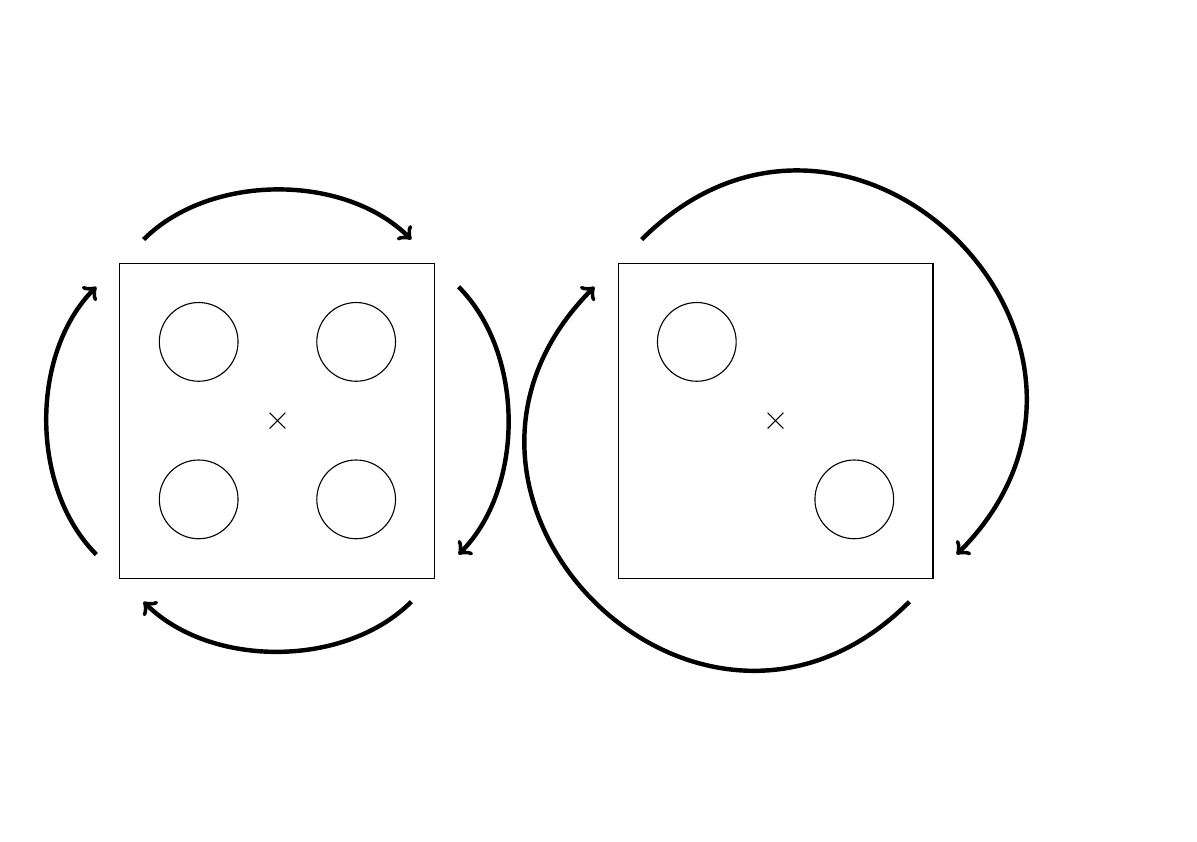
\begin{tikzpicture}
    % Two switches
    % ---------------------
    \draw (0,0) rectangle (4,4);
    \draw (2.1,1.9)--(1.9,2.1);
    \draw (2.1,2.1)--(1.9,1.9);
    \draw (1,3) circle (0.5);
    \draw (3,1) circle (0.5);
    \draw[ultra thick, ->] (0.3, 4.3) to[out=45, looseness=1.7, in=45] (4.3,0.3);
    \draw[ultra thick, ->] (3.7,-0.3) to[out=225, looseness=1.7, in=225] (-0.3, 3.7);

    % Four switches
    % ---------------------
    \draw[xshift=-18em] (0,0) rectangle (4,4);
    \draw[xshift=-18em] (2.1,1.9)--(1.9,2.1);
    \draw[xshift=-18em] (2.1,2.1)--(1.9,1.9);
    \draw[xshift=-18em] (1,1) circle (0.5);
    \draw[xshift=-18em] (1,3) circle (0.5);
    \draw[xshift=-18em] (3,1) circle (0.5);
    \draw[xshift=-18em] (3,3) circle (0.5);
    \draw[xshift=-18em, ultra thick, ->] (0.3, 4.3) to[out=45, looseness=0.9, in=135] (3.7,4.3);
    \draw[xshift=-18em, ultra thick, ->] (4.3,3.7) to[out=-45, looseness=0.9, in=45] (4.3,0.3);
    \draw[xshift=-18em, ultra thick, ->] (3.7, -0.3) to[out=-135, looseness=0.9, in=-45] (0.3,-0.3);
    \draw[xshift=-18em, ultra thick, ->] (-0.3, 0.3) to[out=-225, looseness=0.9, in=-135] (-0.3,3.7);
  \end{tikzpicture}
  \caption[Illustration of Winkler's Spinning Switches and a two-switch analog.]{
    An illustration of Winkler's Spinning Switches puzzle and a two-switch analog.
  }
  \label{fig:twoSwitches}
\end{figure}

In order to bootstrap the two-switch solution into a four-switch solution,
we must notice two things: \begin{enumerate}
  \item First, if we can get two switches along each diagonal into the same state
  respectively, then we can solve the puzzle by toggling both diagonals
  (all four switches),
  followed both switches in a single diagonal,
  and lastly both diagonals again.
  In this (sub-)strategy, toggling both switches along a diagonal is
  equivalent to toggling a single single switch in the two-switch analog.

  \item Second, we can get both diagonals into the same state at some point
  by toggling a switch from each diagonal (two switches on any side of square),
  followed by a single switch from one diagonal,
  followed by again toggling a switch from each diagonal.
\end{enumerate}

We will interleave these strategies in a particular way, following the notation
of Rabinovich \cite{Rabinovich2022}.

\begin{definition}
  Given two sequences $A = \{a_i\}_{i=1}^N$ and $B = \{b_i\}_{i=1}^M$, we can
  define the \textbf{interleave} operation as \begin{align}
    A \circledast B &= (A,b_1,A,b_2,A,\dots,b_M,A) \\
      &= (
      \underbrace{a_1, a_2, \dots, a_N}_A,
      b_1,
      \underbrace{a_1, a_2, \dots, a_N}_A,
      b_2,
      \underbrace{a_1, a_2, \dots, a_N}_A,
      \dots,
      b_M,
      \underbrace{a_1, a_2, \dots, a_N}_A).
  \end{align} which has length $(M+1)N + M = MN + M + N$.
\end{definition}

Typically it is useful to interleave two strategies when
$A$ solves the puzzle given that the switches are in a particular state, and
$B$ gets the switches into that particular state.
We also need $A$ not to ``interrupt'' what $B$ is doing.
In the problem of four switches on a square table,
$B$ will ensure that the switches are in the same state within each diagonal,
and $A$ will turn on the light when that's the case.
Moreover, $A$ does not change the state \textit{within} either diagonal.

\begin{proposition}
  There exists a fifteen-move strategy that guarantees that the light in
  Winkler's puzzle turns on.
  \label{prop:WinklersSolution}
\end{proposition}
\begin{proof}
  We begin by formalizing the two strategies. We will say that the first
  strategy $S_1$ where we toggle the two switches in a diagonal together
  will consist of the following three moves: \begin{enumerate}
    \item Switch \textbf{a}ll of the bulbs ($A$).
    \item Switch the \textbf{d}iagonal consisting of the upper-left and lower-right bulbs ($D$).
    \item Switch \textbf{a}ll of the bulbs ($A$).
  \end{enumerate}
  We will say that the second strategy $S_2$ where we get the two switches
  within each diagonal into the same state consists of the following three
  moves: \begin{enumerate}
    \item Switch both switches on the left \textbf{s}ide ($S$).
    \item Switch \textbf{one} switch ($1$).
    \item Switch both switches on the left \textbf{s}ide ($S$).
  \end{enumerate}
  Then the $15$ move strategy is \begin{equation}
    S_1 \circledast S_2 = (A, S, A, D, A, S, A, 1, A, S, A, D, A, S, A)
  \end{equation}
\end{proof}

We will generalize this construct in
Theorem \ref{thm:switchingStrategyDecomposition},
which offers a formal proof that this strategy works.

(It is worth briefly noting that $S_1 \circledast S_2$ is the fourth
\textit{Zimin word} (also called a \textit{sequipower}),
an idea that comes up in the study of combinatorics on words.)

\subsection{Generalizing switches}
\label{sec:GeneralizingSwitches}
Two kinds of switches are considered by Bar Yehuda, Etzion, and Moran in 1993
\cite{BarYehuda1993}: switches with a single ``on'' position that behave like
$n$-state roulettes ($\mathbb Z_n$) and switches that behave like
the finite field $\mathbb F_q$, both on a rotating $k$-gonal table.
We generalize this notion further by considering switches that behave like
arbitrary finite groups.

\begin{example}
In Figure \ref{fig:S3Switch}, we provide a schematic for a switch that behaves
like the symmetric group $S_3$.
It consists of three identical-looking parts that need to be
arranged in a particular order in order for the switch to be on.

We could also construct a switch that behaves like the dihedral group of the
square, $D_8$.
This switch might look like a flat, square prism that can slot into a square hole,
such that only one of the $|D_8| = 8$ rotations of the prism completes the circuit.
\label{ex:S3D8Schematics}
\end{example}

\begin{figure}
  \center{
  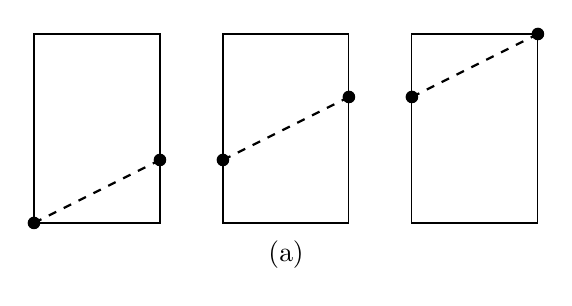
\begin{tikzpicture}[scale=0.8]
    \draw (0,0) rectangle ++(2,3);
    \draw[dashed,thick] (0,0) -- ++(2,1);
    \fill (0,0) circle (0.1);
    \fill (2,1) circle (0.1);

    \draw (3,0) rectangle ++(2,3);
    \draw[dashed,thick] (3,1) -- ++(2,1);
    \fill (3,1) circle (0.1);
    \fill (5,2) circle (0.1);

    \draw (6,0) rectangle ++(2,3);
    \draw[dashed,thick] (6,2) -- ++(2,1);
    \fill (6,2) circle (0.1);
    \fill (8,3) circle (0.1);
    \node at (4, -1/2) {(a)};
  \end{tikzpicture}
  }

  \noindent
  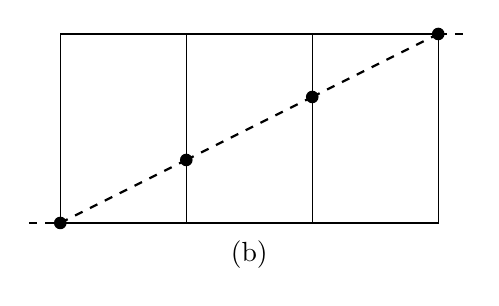
\begin{tikzpicture}[scale=0.8]
    \draw[dashed,thick] (-0.5,0) -- (0,0);
    \fill (0,0) circle (0.1);

    \draw (0,0) rectangle ++(2,3);
    \draw[dashed,thick] (0,0) -- ++(2,1);
    \fill (2,1) circle (0.1);

    \draw (2,0) rectangle ++(2,3);
    \draw[dashed,thick] (2,1) -- ++(2,1);
    \fill (4,2) circle (0.1);

    \draw (4,0) rectangle ++(2,3);
    \draw[dashed,thick] (4,2) -- ++(2,1);
    \fill (6,3) circle (0.1);

    \draw[dashed,thick] (6,3) -- (6.5,3);
    \node at (3, -1/2) {(b)};
  \end{tikzpicture}
  ~
  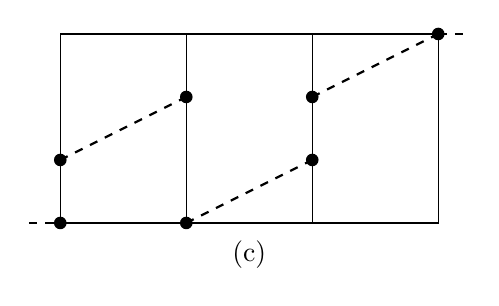
\begin{tikzpicture}[scale=0.8]
    \draw[dashed,thick] (-0.5,0) -- (0,0);
    \fill (0,0) circle (0.1);

    \draw (0,0) rectangle ++(2,3);
    \draw[dashed,thick] (0,1) -- ++(2,1);
    \fill (0,1) circle (0.1);
    \fill (2,2) circle (0.1);

    \draw (2,0) rectangle ++(2,3);
    \draw[dashed,thick] (2,0) -- ++(2,1);
    \fill (2,0) circle (0.1);
    \fill (4,1) circle (0.1);

    \draw (4,0) rectangle ++(2,3);
    \draw[dashed,thick] (4,2) -- ++(2,1);
    \fill (4,2) circle (0.1);
    \fill (6,3) circle (0.1);

    \draw[dashed,thick] (6,3) -- (6.5,3);
    \node at (3, -1/2) {(c)};
  \end{tikzpicture}
  \caption[A schematic for a switch that behaves like $S_3$.]{
    Part (a) shows a simple schematic for the components of a switch that
    behaves like $S_3$, the symmetric group on three letters.
    The three rectangles can be permuted arbitrarily, but only configuration (b)
    completes the circuit. All other configurations fail to
    complete the circuit (e.g., (c)).
  }
  \label{fig:S3Switch}
\end{figure}


\begin{note}
  One subtlety of using a group $G$ to model a switch is that
  both the ``internal state'' of a switch itself and
  the set of ``moves'' or changes are modeled by $G$.
  Therefore it may be useful to think of the state as the underlying set of $G$
  where the moves act via a right group action of $G$ on itself.
\end{note}

The reason that using a group to model a switch is because groups have many
of the properties we would expect in a desirable switch.
\begin{note}
  The axioms for a group $(G, \cdot)$ closely follow what we would expect from
  a switch.
\end{note}
\begin{enumerate}
  \item (Closure) The group $(G, \cdot)$ is equipped with a binary operation,
  $\cdot \colon G \times G \rightarrow G$. That is, for all pairs of elements
   $g_1, g_2 \in G$ their product is in $G$ \begin{equation}
     g_1 \cdot g_2 \in G.
  \end{equation}
  In the context of switches, this
  means that if the switch is in some state $g_1 \in G$ and the puzzle-solver
  applies the move $g_2 \in G$ to it,
  then the resulting state $g_1 \cdot g_2 \in G$ is in the set of possible
  states.
  %
  %
  \item (Identity) There exists an element $\operatorname{id}_G \in G$ such that
  for all $g \in G$, \begin{equation}
    \operatorname{id}_G \cdot g = g \cdot \operatorname{id}_G = g.
  \end{equation}
  This axiom is useful because it means that the puzzle-solver can ``do nothing''
  to a switch and leave it in whatever state it is in.
  Because the identity is a distinguished element in $G$,
  we will also use the convention that
  $\operatorname{id}_G$ is the ``on'' or ``winning'' state for a given switch.
  (It is worth noting that all of the arguments work basically the same way
  regardless of which element is designated as the on state.)
  %
  %
  \item (Inverses) For each element $g \in G$ there exists an inverse element
  $g^{-1} \in G$ such that \begin{equation}
    g \cdot g^{-1} = g^{-1} \cdot g = \operatorname{id}_G.
  \end{equation}
  This axiom states that no matter what state a switch is in,
  there is a move that will transition it into the on state.
  %
  %
  \item (Associativity) Given three elements $g_1, g_2, g_3 \in G$,
  \begin{equation}
    (g_1 \cdot g_2) \cdot g_3 = g_1 \cdot (g_2 \cdot g_3)
  \end{equation}
  This is axiom is not strictly necessary for modeling switches,
  but as we will see in a later definition, it gives us a convenient way to
  describe the conditions for a winning strategy.
  (In Subsection \ref{sub:quasigroupSwitches}, we briefly discuss dropping
  the associativity axiom by considering switches that behave like
  quasigroups with identity.)
\end{enumerate}

% In a similar vein, we could construct a switch that behaves like the dihedral
% group of the square. Perhaps the switch is a thin square prism that fits into a
% square slot in such a way that only one orientation of the prism completes the
% circuit. See Figure \ref{fig:D8Switch} for a simple schematic.
% [A schematic for a switch that looks like $D_4$.]
% Or one could imagine a switch that behaves like the dihedral group of the square,
% $D_8$ where the square has a single, unique orientation that completes the circuit.
% Or abstractly, one could think of each switch as an abstract group element,
% where the puzzle-solver can multiply by anything they like.

\subsection{Generalizing spinning}
We can also consider generalizations of ``spinning'' the switches.
In particular, we will adopt the generalization from
Ehrenborg and Skinner's \cite{Ehrenborg1995} 1995 paper, which use
arbitrary faithful group actions to permute the switches.
In particular, they provide a criterion that determines which group actions
yield a winning strategy in the case of a given number of ``ordinary'' switches
(those that behave like $\mathbb Z_2$).
Rabinovich \cite{Rabinovich2022} stretches these results a bit further and
looks at faithful linear group actions on collections of switches that behave
are modeled as a finite dimensional vector space over a finite field.
We build on this result in the context of more general switches.

\section{A wreath product model}
\label{sec:WreathModel}
Recall that Peter Winkler's Spinning Switches puzzle consists of four two-way
switches on the corners of a rotating square table.
The behavior of the switches are naturally modeled as $\mathbb Z_2$, and
the rotating table is modeled as the cyclic group $C_4$.
The abstraction that takes these two groups and creates a model for the
underlying puzzle is the wreath product: that is Winkler's puzzle behaves like
the wreath product of $\mathbb Z_2$ by $C_4$.

\subsection{Modeling generalized spinning switches puzzles}
We don't evoke wreath products arbitrarily: we use them because they are the
right abstraction to model a generalized spinning switches puzzle where
$G$ describes the behavior of the switches,
$\Omega$ describes the positions of the switches, and
the action of $H$ on $\Omega$ models the ways the adversary can permute the switches.

\begin{definition}[\cite{Rotman1999}]
  Let $G$ and $H$ be groups,
  let $\Omega$ be a finite $H$-set, and
  let $K = \prod_{\omega \in \Omega} G_\omega$, where $G_\omega \cong G$
  for all $\omega \in \Omega$.
  Then the \textbf{wreath product} of $G$ by $H$ denoted by $G \wr H$,
  is the semidirect product of $K$ by $H$,
  where $H$ acts on $K$ by $h \cdot (g_\omega) = g_{h^{-1}\omega}$ for $h \in H$
  and $g_\omega \in G_\omega$.
  The normal subgroup $K$ of $G \wr H$ is called
  the \textbf{base} of the wreath product.

  The group operation is $(k, h) \cdot (k', h') = (k(h \cdot k'), hh')$
\end{definition}

An element of $(k, h) \in G \wr H$ represents a turn of the game:
The puzzle-solver chooses an element of the base $k \in K$ to indicate
how they want to modify each of their switches
and then their adversary chooses $h \in H$ and acts with $h$ on $\Omega$ to
permute the switches.

\begin{example}
  Consider the setup in the Winkler's Spinning Switches the puzzle, which
  consists of two-way switches ($\mathbb Z_2$) on the corners of a rotating
  square,
  $C_4 \cong \langle 0^\circ, 90^\circ, 180^\circ, 270^\circ \rangle$.
  The game itself corresponds to the wreath product $\mathbb Z_2 \wr C_4$.
  We will use the convention that the base of the wreath product, $K$, is
  ordered upper-left, upper-right, lower-right, lower-left, and that the group
  action is specified by degrees in the clockwise direction.

  Consider the following two turns:
  \begin{enumerate}
    \item During the first turn,
    the puzzle-solver toggles the upper-left and lower-right switches, and
    the adversary rotates the table $90^\circ$ clockwise.
    This is represented by the element \begin{equation}
      ((1,0,1,0), 90^\circ) \in \mathbb Z_2 \wr C_4.
    \end{equation}
    \item During the second turn,
    the puzzle-solver toggles the upper-left switch, and
    the adversary rotates the table $90^\circ$ clockwise.
    This is represented by the element \begin{equation}
      ((1,0,0,0), 180^\circ) \in \mathbb Z_2 \wr C_4.
    \end{equation}
  \end{enumerate}
  %
  As illustrated in Figure \ref{fig:WreathProduct},
  the net result of these two turns is the same as
  a single turn where the puzzle-solver toggles the
  upper-left, upper-right, and lower-left
  switches and the adversary rotates the board $270^\circ$ clockwise.

  \begin{figure}
    \center
    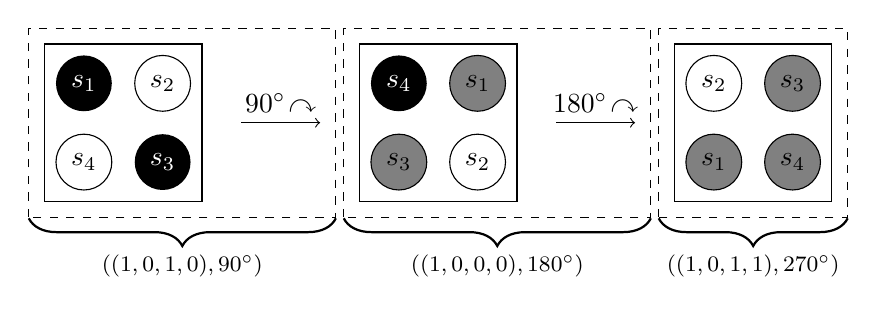
\begin{tikzpicture}
      \draw[dashed] (-0.2,-0.2) rectangle (3.7,2.2);
      \draw [thick,decorate,decoration={brace,amplitude=10pt},yshift=-0.4pt]
        (3.7,-0.2) -- (-0.2,-0.2) node[black,midway,yshift=-0.6cm] {\footnotesize $((1,0,1,0), 90^\circ)$};

      \draw[dashed] (3.8,-0.2) rectangle (7.7,2.2);
      \draw [thick,decorate,decoration={brace,amplitude=10pt},yshift=-0.4pt]
        (7.7,-0.2) -- (3.8,-0.2) node[black,midway,yshift=-0.6cm] {\footnotesize $((1,0,0,0), 180^\circ)$};

      \draw[dashed] (7.8,-0.2) rectangle (10.2,2.2);
      \draw [thick,decorate,decoration={brace,amplitude=10pt},yshift=-0.4pt]
        (10.2,-0.2) -- (7.8,-0.2) node[black,midway,yshift=-0.6cm] {\footnotesize $((1,0,1,1), 270^\circ)$};

      \draw (0,0) rectangle (2,2);
      \node[circle,fill,text=white] at (1/2,3/2) {$s_1$};
      \node[circle,draw] at (3/2,3/2) {$s_2$};
      \node[circle,fill,text=white] at (3/2,1/2) {$s_3$};
      \node[circle,draw] at (1/2,1/2) {$s_4$};
      \draw[->] (2.5,1) -- node[above] {$90^\circ \! \curvearrowright$} (3.5,1) ;

      \draw (4,0) rectangle (6,2);
      \node[circle,fill,text=white] at (9/2,3/2) {$s_4$};
      \node[circle,draw,fill=gray] at (11/2,3/2) {$s_1$};
      \node[circle,draw] at (11/2,1/2) {$s_2$};
      \node[circle,draw,fill=gray] at (9/2,1/2) {$s_3$};

      \draw[->] (6.5,1) -- node[above] {$180^\circ \! \curvearrowright$} (7.5,1) ;

      \draw (8,0) rectangle (10,2);
      \node[circle,draw] at (17/2,3/2) {$s_2$};
      \node[circle,draw,fill=gray] at (19/2,3/2) {$s_3$};
      \node[circle,draw,fill=gray] at (19/2,1/2) {$s_4$};
      \node[circle,draw,fill=gray] at (17/2,1/2) {$s_1$};
    \end{tikzpicture}
    \caption[A wreath product interpretation of a spinning switches puzzle.]{
      An illustration of two turns each in Winkler's Spinning Switches puzzle,
      modeled as elements of a wreath product.
    }
    \label{fig:WreathProduct}
  \end{figure}

  The multiplication under the wreath product agrees with this: \begin{align*}
    ((1,0,1,0), 90^\circ) \cdot ((1,0,0,0), 180^\circ)
    &= ((1,0,1,0) + \underbrace{90^\circ \cdot (1,0,0,0)}_{(0,0,0,1)}, 90^\circ + 180^\circ) \\
    &= ((1,0,1,1), 270^\circ)
  \end{align*}
\end{example}

As suggested earlier, it is occasionally useful to designate a particular state
of the switches as the winning state. We will use the
convention that the lightbulb turns on when all of the switches are equal to the
identity, that is $\mathrm{id}_K \in K$.
It is worth noting, however, that the existence of a winning strategy does not
depend on a particular choice in the winning state.
Instead, we will see that a winning strategy is equivalent to a choice of moves
that will walk over all of the possible configuration states, regardless of the
choice of the adversaries spin.

\subsection{Switching strategy}

We will begin by formalizing the notation of a winning strategy in a
generalized spinning switches puzzle. Informally, this is
a sequence of moves that the puzzle-solver can make that will put the switches
into every possible state, which ensures the the winning state is reached
regardless of the initial (hidden) state of the switches.

\begin{definition}
  A \textbf{switching strategy} for $G \wr H$ is a finite sequence of elements
  in the base $K$,
  $\{k_i \in K\}_{i=1}^N$,
  such that for every sequence of elements in $H$, ${\{h_i \in H\}_{i=1}^N}$,
  \begin{equation}
    p(\{
      \underbrace{e_{G \wr H}}_{m_0},
      \underbrace{(k_1, h_1)}_{m_1},
      \underbrace{(k_1, h_1)\cdot(k_2, h_2)}_{m_2},
      \dots,
      \underbrace{(k_1, h_1)\cdot(k_2, h_2)\cdots(k_N, h_N)}_{m_N}
    \}) = K.
  \end{equation}
  where $p \colon G \wr H \rightarrow K$ is the projection map from the
  wreath product onto its base.
\label{def:switchingStrategy}
\end{definition}

This definition is useful because it puts the problem into purely algebraic
terms. It is also useful because it abstracts away the initial state of the
switches: regardless of the initial state $k \in K$, a existence of a switching strategy
means that its inverse $k^{-1} \in K$ appears in the sequence.
(This follows the convention that $\mathrm{id}_K \in K$ is designated as the
winning state. If $k'$ is chosen to be the winning state, then the sequence
must contain $k^{-1}k'$ .)

\begin{proposition}
  A finite sequence of moves is guaranteed to reach the winning
  state if and only if it is a switching strategy.
\end{proposition}
\begin{proof}
  Without loss of generality, say that the winning state for the switches is
  $\mathrm{id}_K$.
  In the puzzle, we have an initial (hidden) state, $k$.
  Thus, after the $i$-th move, the wreath product
  element that represents the state of the switches is \begin{equation}
    p\left((k, \mathrm{id}_H)\cdot(k_1, h_1)\cdot(k_2, h_2)\cdots(k_i, h_i)\right)
    = k \cdot p\left((k_1, h_1)\cdot(k_2, h_2)\cdots(k_i, h_i)\right),
  \end{equation} by associativity. We can factor out the first term because
  the ``spin'' is $\mathrm{id}_H$, which acts trivially:
  ${(k, \mathrm{id}_H) \cdot (k', h') = (kk', h')}$

  Since $k$ is arbitrary the projection map must be a surjection onto $K$ for
  every adversarial sequence to ensure that it contains $k^{-1}$.

  The initial state can be any $k \in K \setminus \{\mathrm{id}_K\}$,
  and this isn't known to the puzzle-solver.
  In order to reach the winning state, there must exist some $i$, such that
  $p\left((k_1, h_1)\cdot(k_2, h_2)\cdots(k_i, h_i)\right) = k^{-1}$.
  For any choice of $k$ and adversarial sequence $\{h_i \in H\}_{i=1}^N$.
\end{proof}

It's also worth noting that this model can be thought of as a random model or an
adversarial model: the sequence $\{h_i \in H\}$ can be chosen
randomly at any point, or it can be chosen deterministically
after the sequence $\{k_i \in K\}$ is specified.

\subsection{Bounds on the length of switching strategies}

One useful consequence of this definition is that it quite straightforward to
prove certain propositions. For example, the minimum length for a switching strategy
has a simple lower bound.
\begin{proposition}
  Every switching strategy $\{k_i \in K\}_{i=1}^{N}$ is a sequence of
  length at least ${|K| - 1}$.
\end{proposition}
\begin{proof}
  This follows from an application of the Pigeonhole Principle. Because the set
  \begin{equation}
    \{e_{G \wr H}, (k_1, h_1), (k_1, h_1)\cdot(k_2, h_2), \cdots, (k_1, h_1)\cdot(k_2, h_2)\cdots(k_N, h_N)\}
  \end{equation}
  has at most $N+1$ elements. In order for the projection to be equal to $K$,
  \begin{equation}
    p(\{e_{G \wr H}, (k_1, h_1), (k_1, h_1)\cdot(k_2, h_2), \cdots, (k_1, h_1)\cdot(k_2, h_2)\cdots(k_N, h_N)\}) = K,
  \end{equation} it must be the case that $N+1 \geq |K|$.
  Therefore $N \geq |K| - 1$.
\end{proof}

Minimal length switching strategies are common, so we give them a name.
\begin{definition}
  A \textbf{minimal switching strategy} for $G \wr H$ is a switching strategy
  of length $N = |K| - 1.$
\end{definition}

In practice, every wreath product known by the author to have a switching
strategy also has a known minimal switching strategy.
In Section \ref{sec:OpenQuestions}, we ask whether this property always holds.

% 2DO: uncomment and fix this section.
% \subsection{Upper bound for the length of switching strategies}
% Of course, switching strategies can be arbitrarily long.
% For instance, adding any prefix or suffix to a switching strategy again
% results in a switching strategy. However, given a long switching strategy, we
% may want to be able to detect when a shorter one exists.

% We begin with an example that illustrates how this works.

% \begin{proposition}
%   Whenever $G \wr H$ has a switching strategy, it also has a switching strategy
%   of length $N < 2^{|K/H|-1}$, where $K/H$ is the set of equivalence classes of
%   $K$, where $k \sim k'$ if $k = k'h$ for some $h \in H$.
% \end{proposition}

% \begin{proof}
%   % (?) Nondeterministic finite automaton? (?)
%   % Let $K$ act on an element $[k'] \in K/H$ by
%   % $[k']\cdot k = \{[k'(h\cdot k)] : h \in H\}$.
% \end{proof}

\section{Reductions}
\label{sec:Reductions}
In this section, we develop examples of generalized spinning switches puzzles
that do not have switching strategies using three techniques:
directly, by a reduction on switches, or by a reduction on spinning.
%
\subsection{Puzzles known to have no switching strategies}
Our richest collection of known puzzles without switching strategies comes from
a theorem of Rabinovich, which models switches as a vector space over
a finite field.
\begin{theorem} \cite{Rabinovich2022}
  Assume that a finite ``spinning'' group $H$ acts linearly and faithfully on
  a collection of switches that behave like a vector space
  $V$ over a finite field $\mathbb F_q$ of characteristic $p$.
  Then the resulting puzzle has a switching strategy if and only if $H$ is a
  $p$-group.
  \label{thm:Rabinovich}
\end{theorem}
It's worth noting that Rabinovich's switches are less general than arbitrary
finite groups, but the ``spinning'' is more general: in addition to permuting
the switches, the group action might add linear combinations of them as well.
\begin{example}
  By the theorem of Rabinovich \cite{Rabinovich2022},
  the game $\mathbb Z_2 \wr C_3$ does not have a
  switching strategy. In Rabinovich's notation, the vector space of switches
  is $\mathbb Z_2^3$ over the field $\mathbb F_2 = \mathbb Z_2$, and
  $C_3$ has $3$ elements and therefore is not a $2$-group.
  \label{ex:NoSolutionZ2C3}
\end{example}

The wreath product $\mathbb Z_2 \wr C_3$ is perhaps the simplest example of a
generalized spinning switches puzzle without a switching strategy,
so we will continue to use it as a basis of future examples.

\subsection{Reductions on switches}
With Theorem \ref{thm:Rabinovich} providing a family of wreath products without
switching strategies, we now introduce a theorem that allows us to
describe large families of wreath products that also do not have switching
strategies.
\begin{theorem}
  If $G \wr H$ does not have a switching strategy and there exists a group $G'$
  and a surjective homomorphism $\varphi \colon G' \rightarrow G$,
  then ${G'} \wr H$ does not have a switching
  strategy.
  \label{thm:SwitchReduction}
\end{theorem}
\begin{proof}
  We will prove the contrapositive, and suppose that $G' \wr H$ has base $K'$
  and a switching strategy $\{k'_i \in K'\}_{i=1}^N$.

  The homomorphism
  $\varphi\colon G' \mapsto G$
  extends coordinatewise to
  $\varphi \colon K' \mapsto K$,
  which further extends in the first coordinate to $G \wr H$:
  $\varphi(k,h) := (\varphi(k), h)$.

  It is necessary to verify that $\varphi\colon G' \wr H \rightarrow G \wr H$
  is indeed a homomorphism.
  \begin{align*}
    \varphi((k'_\alpha, h_\alpha)) \cdot \varphi((k'_\beta, h_\beta))
    &= (\varphi(k'_\alpha), h_\alpha) \cdot (\varphi(k'_\beta), h_\beta) \\
    &= (\varphi(k'_\alpha)(h_\alpha\cdot\varphi(k'_\beta)), h_\alpha h_\beta) \\
    &= (\varphi(k'_\alpha)\varphi(h_\alpha\cdot k'_\beta), h_\alpha h_\beta) \\
    &= (\varphi(k'_\alpha(h_\alpha\cdot k'_\beta)), h_\alpha h_\beta) \\
    &= \varphi((k'_\alpha(h_\alpha\cdot k'_\beta), h_\alpha h_\beta)) \\
    &= \varphi((k'_\alpha, h_\alpha) \cdot (k'_\beta, h_\beta))
  \end{align*}

  Therefore the sequence $\{\varphi(k'_i) \in K\}_{i=1}^N$ is a
  switching strategy on $G \wr H$, because the quotient map
  $\varphi \colon G' \rightarrow G$
  (and thus $\varphi \colon K' \rightarrow K$)
  is injective.
\end{proof}
\begin{example}
  We know that $\mathbb Z_2 \wr C_3$ doesn't have a switching strategy.
  This means that $\mathbb Z_6 \wr C_3$ does not have a switching strategy either,
  as illustrated in Figure \ref{fig:Z2C3}.
  \begin{figure}
    \center
    \includegraphics{assets/tikz_Z2C3.pdf}
    \caption[A reduction from a six-way switch to a two-way switch]{
      A reduction on switches:
      $\mathbb Z_6 \wr C_3$ reduces to $\mathbb Z_2 \wr C_3$,
      which is known not to have a switching strategy.
    }
    \label{fig:Z2C3}
  \end{figure}
\end{example}
\subsection{Reductions on spinning}
We can do two similar reductions on the ``spinning'' group of a wreath product.
These theorems say that if a given wreath product $G \wr H$ does not have a
switching strategy, then a similar wreath product $G \wr H'$ with a
``more complicated'' spinning group $H'$ will not have a switching strategy
either.
\begin{theorem}
  If $G \wr H$ does not have a switching strategy,
  and $\varphi \colon H \hookrightarrow H'$ is an embedding of $H$ into $H'$,
  then $G \wr H'$ does not have a switching strategy.
  \label{thm:SpinReduction}
\end{theorem}
\begin{proof}
  Again we will prove the contrapositive.
  Assume that $G \wr H'$ does have a switching strategy,
  $\{k_i\}_{i=1}^N$. Then by definition, for any sequence
  $\{h'_i\}_{i=1}^N$, the projection of the sequence \begin{equation}
    p(\{(k_1, h'_1)\cdot(k_2, h'_2)\cdots(k_i, h'_i)\}_{i=1}^N) = K,
  \end{equation} and in particular this is true when $h'_i$ is restricted to be
  in the subgroup $\operatorname{Im}(\varphi) \leq H'$.
  Thus a switching strategy for $G \wr H'$ is also a valid switching strategy
  for $G \wr H$.
\end{proof}

\begin{example}
  Consider the wreath product $\mathbb Z_2 \wr_{\Omega_6} C_3$ where
  $\Omega'$ consists of six switches on the corners of a hexagon as
  illustrated in Figure \ref{fig:Z2C6}.
  We know that $\mathbb Z_2 \wr_{\Omega_6} C_3$ does not have a switching
  strategy, by Theorem \ref{thm:Rabinovich}, therefore
  $\mathbb Z_2 \wr_{\Omega_6} C_3$ cannot have a switching strategy either, by
  Theorem \ref{thm:SpinReduction}.
\end{example}

\begin{figure}
  \center
  \includegraphics{assets/tikz_Z2C6.pdf}
  \caption[A reduction from $60^\circ$ rotations to $120^\circ$ rotations.]{
    If there were a solution to $\mathbb Z_2 \wr_{\Omega_6} C_6$,
  then there would be a solution to $\mathbb Z_2 \wr_{\Omega_6} C_3$.
  }
\label{fig:Z2C6}
\end{figure}

In the above example, we noted that $\mathbb Z_2 \wr_{\Omega_6} C_6$ does
not have a switching strategy because $\mathbb Z_2 \wr_{\Omega_6} C_3$ is
known not to have one. However, there is another obstruction: the fact that
the generalized spinning switches puzzle $\mathbb Z_2 \wr C_3$ on a triangle
is known not to have a switching strategy. That is, we cannot guarantee that
the triangle that is embedded in the hexagon as ``every other'' switch
is ever in the all ``on'' state.

The following theorem abstracts this idea.
\begin{theorem}
  Suppose that $H$ and $H'$ are groups,
  $\varphi \colon H \hookrightarrow H'$ is an embedding of $H$ into $H'$,
  \begin{equation}
    \operatorname{Orb}(\omega)
      = \{\omega \cdot a : a \in \operatorname{Im}(\varphi) \} \subseteq \Omega
  \end{equation}
  be the (right) orbit of $\omega \in \Omega$ under $\operatorname{Im}(\varphi)$.
  If $G \wr_{\operatorname{Orb}(\omega)} H$ does not have a switching strategy,
  then $G \wr_\Omega H'$ cannot have a switching strategy either.
  \label{thm:SpinReduction2}
\end{theorem}
\begin{proof}
  We start by making the contrapositive assumption that $G \wr_\Omega H'$
  has a switching strategy ${\{k_i \in K\}_{i=1}^N}$,
  and we consider the projection
  $p_\omega \colon K \rightarrow K_\omega$ where
  \begin{equation}
    K = \prod_{\omega' \in \Omega} G_{\omega'}
    \hspace{1cm}\text{and}\hspace{1cm}
    K_{\omega} = \prod_{\omega' \in \operatorname{Orb}(\omega)} G_{\omega'}.
  \end{equation}

  Then $\{p_\omega(k_i) \in K_\omega\}_{i=1}^N$ is a switching strategy for
  $G \wr_{\operatorname{Orb}(\omega)} H$, since the projection is a surjective
  map.
\end{proof}

\begin{example}
  We know that $\mathbb Z_2 \wr C_3$ doesn't have a switching strategy.
  This means that $\mathbb Z_2 \wr C_6$ does not have a switching strategy either,
  as illustrated in Figure \ref{fig:Z2C6_2}.
\end{example}
\begin{figure}
  \center
  \includegraphics{assets/tikz_Z2C6_2.pdf}
  \caption[A reduction from a hexagonal table to a triangular table.]{
    We know that $\mathbb Z_2 \wr_\Omega C_6$ cannot have
    a switching strategy, because that would imply a switching strategy for
    $\mathbb Z_2 \wr_{\Omega'} C_3$, where $\Omega'$
    is the orbit of the top switch rotations of multiples of $120^\circ$.
  }
  \label{fig:Z2C6_2}
\end{figure}

Now that we've proven that large families of wreath products do not have
switching strategies, it's worthwhile to construct families of wreath products
that do have switching strategies.
%%%%%%%%%%%%%%%%%%%%%%%%%%%%%%%%%%%%%%%%%%%%%%%%%%%%%%%%%%%%%%%%%%%%%%%%%%%%%%
%
% Switching strategies on p-groups
%
%%%%%%%%%%%%%%%%%%%%%%%%%%%%%%%%%%%%%%%%%%%%%%%%%%%%%%%%%%%%%%%%%%%%%%%%%%%%%%
\section{Switching strategies on \texorpdfstring{$p$}{p}-groups}
\label{sec:pGroupStrategy}
In this section, we'll develop a broad family of switching strategies,
namely those where $G$ and $H$ (and thus $G \wr H$) are $p$-groups.
\subsection{Switching strategy decomposition}

Our first constructive theorem provides a technique that can be used to
construct switching strategies for switches that behave like a group $G$ in
terms of a normal group and its corresponding quotient group.
\begin{theorem}
  The wreath product $G \wr H$ has a switching strategy if there exists a
  normal subgroup $N \trianglelefteq G$ such that both $N \wr H$ and
  $G/N \wr H$ have switching strategies.
\label{thm:switchingStrategyDecomposition}
\end{theorem}
\begin{proof}
  Let \[
    S_{G/N} = \{k_i^{G/N} \in K_{G/N}\}
    \hspace{1cm}\text{and}\hspace{1cm}
    S_{N} = \{k_i^N \in K_{N}\}
  \] denote the switching strategies for ${G/N \wr H}$ and ${N \wr H}$
  respectively.

  We ultimately would like to interleave these two strategies,
  but $k_i^{G/N} \not\in K_G$. To find the appropriate analog,
  we partition $G$ into $[G : N] = m$ right cosets of $N$, \begin{equation}
    G = Ng_1 \sqcup Ng_2 \sqcup \dots \sqcup Ng_m,
  \end{equation} each with a chosen representative in $G$.
  Now we define a map $r \colon G/N \rightarrow G$ that chooses the chosen
  representative of the coset, and extends coordinatewise. We use this map to
  define a sequence $S = \{r(k_i^{G/N}) \in K_G\}$.

  We claim that these two sequences interleaved, $S_N \circledast S$, is a
  switching strategy for $G \wr H$. To prove this claim, we observe two facts:
  \begin{enumerate}
    \item Multiplying by elements of $S_N$ will not change cosets and will walk
    through every element of its coset.
    \item Multiplying by elements of $S$ will walk through all cosets.
  \end{enumerate}
  Therefore the interleaved sequence will walk through all elements of each
  coset, and thus is surjective onto $K$.
\end{proof}

\subsection{Construction of switching strategies on \texorpdfstring{$p$}{p}-groups}
With the decomposition from Theorem \ref{thm:switchingStrategyDecomposition}
established, we can now construct a switching strategy on all finite $p$-groups.

\begin{theorem}
  If $H$ is a finite $p$-group that acts faithfully on $\Omega$,
  then the wreath product
  $G \wr H$ has a switching strategy whenever $|G| = p^n$ for some $n$.
  \label{thm:pGroupStrategy}
\end{theorem}
\begin{proof}
  We will use the fact that if $|G| = p^n$,
  then either $G \cong \mathbb{Z}_p$ or $G$ is not simple.

  If $n = 1$, then $G \cong \mathbb{Z}_p \cong \mathbb F_p$, so there exists a
  switching strategy by Theorem \ref{thm:Rabinovich}. This is because $H$
  permutes the coordinates of $V = \mathbb F_p^{|\Omega|} \cong K$, and so it is a
  linear action on the vector space, and so it has a switching strategy by
  Theorem \ref{thm:Rabinovich}.

  Otherwise, $G$ is not simple. This means that $G$ has a proper normal subgroup
  $N$ of order $|N| = p^t$ (with $0 < t < n$)
  and a quotient $G/N$ with order $|G/N| = p^{n-t}$.
  Therefore, by induction on the exponent,
  whenever $G$ and $H$ (and thus $G \wr H$) are $p$-groups,
  then $G \wr H$ has a switching strategy.
\end{proof}

Thus this resolves the situation for switches that behave like $p$-groups on
spinning groups that act faithfully and behave like $p$-groups. This allows us
to fully classify the case of abelian switches.

\subsection{A classification of puzzles with abelian switches}

\begin{theorem}
  If $G$ is an abelian group, and $H$ acts faithfully on $\Omega$, then
  $G \wr_\Omega H$ has a switching strategy if and only if $G$ and $H$ are
  both $p$-groups for the same prime $p$.
\label{thm:classifyAbelianSwitches}
\end{theorem}
\begin{proof}
  One direction is clear: if $G$ and $H$ are both $p$-groups for the same prime
  $p$, then $G \wr H$ has a switching strategy by Theorem \ref{thm:pGroupStrategy}.

  For the other direction, we will consider the contrapositive assumption,
  split into three cases, each time assuming that
  $G$ and $H$ are not both $p$-groups for the same prime $p$.

  First, assume that $G$ is a $p$-group, but $H$ is not a $p$-group. Then by
  Sylow's first theorem, there exists a subgroup $\hat{H} \leq H$ that is a $q$-group
  for some prime $q \neq p$. By Theorem \ref{thm:Rabinovich}, since $q \neq p$,
  $G \wr \hat{H}$ does not have a switching strategy, thus it follows from
  the reduction on spinning given in Theorem \ref{thm:SpinReduction} that
  $G \wr H$ does not have a switching strategy either.

  Second, assume that $H$ is a $p$-group, but $G$ is not a $p$-group. Similarly,
  by Sylow's first theorem, there exists a subgroup $\hat{G} \leq G$ that is
  a $q$-group for some prime $q \neq p$. Since $G$ is abelian, $\hat{G}$ is a
  normal subgroup. By Theorem \ref{thm:Rabinovich}, since $q \neq p$,
  $\hat G \wr H$ does not have a switching strategy, thus it follows from
  the reduction on switches given in Theorem \ref{thm:SwitchReduction} that
  $G \wr H$ does not have a switching strategy either.

  Lastly, assume that there does not exist any $p$ such that $G$ is a $p$-group
  or $H$ is a $p$-group. Then $|G|$ and $|H|$ must have multiple prime divisors,
  so $G$ has a normal subgroup, $\overline G$, that is a $q$-group for some prime $q$, and
  $H$ has a normal subgroup $\overline H$ that is a $r$-group for some prime $r \neq q$.
  $\overline G \wr \overline H$ does not have a switching strategy by Theorem \ref{thm:Rabinovich},
  so $G \wr \overline H$ does not have a switching strategy by Theorem \ref{thm:SwitchReduction},
  so $G \wr H$ does not have a switching strategy by Theorem \ref{thm:SpinReduction}.
\end{proof}

\subsection{A folklore conjecture}
Here we note a conjecture from folklore, which---if true---implies that we have
\textit{almost} solved the problem in its full generality.
\begin{conjecture}[Folklore]
  Almost all groups are $2$-groups.
\end{conjecture}

There are both computational and theoretical bases for this conjecture.
According to the On-Line Encyclopedia of Integer Sequences \cite{oeis},
there are $A000001(2^{10}) = 49487367289$ groups of order $2^{10}$ and there are
$A063756(2^{11}-1) = 49910536613$ groups of order less than $2^{11}$.
This means that more than $99.15\%$ of the groups of order less than $2^{11}$
are of order $2^{10}$.

If this conjecture is true, then most types of switches have switching
strategies on most kinds of faithful finite group actions.
Of course, while most finite groups may be $2$-groups, most mathematicians
are more interested in the other finite groups.
This next section develops two families of examples of switching strategies
where the switches do not behave like $p$-groups.

%%%%%%%%%%%%%%%%%%%%%%%%%%%%%%%%%%%%%%%%%%%%%%%%%%%%%%%%%%%%%%%%%%%%%%%%%%%%%%
%
% Switching strategies on permutations
%
%%%%%%%%%%%%%%%%%%%%%%%%%%%%%%%%%%%%%%%%%%%%%%%%%%%%%%%%%%%%%%%%%%%%%%%%%%%%%%
\section{Switching strategies on other wreath products}
\label{sec:OtherSwitchingStrategies}

Other authors have given switching strategies for various configurations of
generalized spinning switches strategies, but in all of these examples,
the wreath products themselves are $p$-groups: that is,
${|G \wr_\Omega H| = |G|^{|\Omega|} \cdot |H|}$, where $H$ acts faithfully.
In this section we introduce two families of wreath products that have switching
strategies, but are not $p$-groups.

\subsection{The trivial wreath product, \texorpdfstring{$G \wr \mathbf{1}$}{G wreath trivial group}}
The simplest---and least interesting---way to construct a wreath product with
a switching strategy is to remove the adversary (or randomness) altogether,
by letting the spinning group be the trivial group $H = \mathbf{1}$.
Additionally we will consider the case where $|\Omega| = 1$, so there is only
one switch.
Because the adversary cannot ``spin'' the switches at all, the puzzle-solver has
perfect information the entire time.
We will see that whenever $G$ is a finite group,
$G \wr \mathbf{1} \cong G$ has not just one switching strategy, but many.

\begin{proposition}
  The wreath product $G \wr \mathbf{1}$ has $(|G|-1)!$ minimal switching
  strategies.
  \label{prop:countingTrivialSS}
\end{proposition}
\begin{proof}
  There are $(|G| - 1)!$ permutations of $G \setminus \{\mathrm{id}_G\}$, and
  we claim each one corresponds to a minimal switching strategy. Namely,
  if $(k_1, k_2, \dots, k_{|G|-1})$ is such a permutation, then
  the sequence $\{k'_i\}_{i=1}^{|G|-1}$ where $k'_1 = k_1$ and
  $k'_i = k_{i-1}^{-1}k_i$ is a switching strategy on $G \wr \mathbf{1}$.

  Then we claim by induction that
  $(k'_1, \mathrm{id})\cdot(k'_2, \mathrm{id})\cdots(k'_j, \mathrm{id}) = (k_j, \mathrm{id})$.
  By construction, the base case is true when $j = 1$. If the claim holds up to
  $j-1$, then \begin{equation}
    \underbrace{
      (k'_1, \mathrm{id})\cdot(k'_2, \mathrm{id})\cdots(k'_{j-1}, \mathrm{id})
    }_{(k_{j-1}, \mathrm{id})}
    (k'_j, \mathrm{id})
    = (k_{j-1}, \mathrm{id})(k_{j-1}^{-1}k_j, \mathrm{id})
    = (k_j, \mathrm{id}),
  \end{equation} as desired.
  Thus the projection of the partial products is
  \begin{align}
    &p(\{
      \underbrace{e_{G \wr \mathbf{1}}}_{m_0},
      \underbrace{(k'_1, h_1)}_{m_1},
      \underbrace{(k'_1, h_1)\cdot(k'_2, h_2)}_{m_2},
      \cdots,
      \underbrace{(k'_1, h_1)\cdot(k'_2, h_2)\cdots(k'_{|G|-1}, h_{|G|-1})}_{m_{|G|-1}}
    \}) \\
    & \hspace{1cm} =
    p(\{
      e_{G \wr \mathbf{1}},
      (k_1, \mathrm{id}),
      (k_2, \mathrm{id}),
      \cdots,
      (k'_{|G|-1}, \mathrm{id})
    \}) \\
    & \hspace{1cm} = \{e_{G \wr \mathbf{1}}, k_1, k_2, \cdots,k_{|G|-1}\} = K,
  \end{align}
  where $\{k_1, k_2, \dots, k_{|G|-1}\}$ spans
  $G \setminus \{\mathrm{id}_G\} \cong K \setminus \{\mathrm{id}_K\}$ by
  assumption.
\end{proof}

While the trivial wreath product is a useful example to keep in mind for
generating counterexamples, we're generally more interested in the situation
where the adversary permutes the switches to create uncertainty for the
puzzle-solver.

\subsection{Two interchangeable groups generated by involutions}

In this section, we will construct a switching strategy for the generalized
spinning switches puzzle $G \wr H$
that consists of two switches each behaving like
a group $G$, generated by involutions, together with a nontrivial spinning
action $H$.
(See, for example, Figure \ref{fig:S3Switch} which illustrates switches that
behave like $S_3 = \langle (12), (13)\rangle$)

This strategy relies on the fact that because each generator is its own
inverse, applying a generator to the first switch or the second switch
has no effect on their difference.

This switching strategy has two parts.
The first part ensures that the two switches have every possible difference.
The second part shows that we can get the first switch
(with respect to the projection onto $K$) to take on every possible value
without changing the difference between the switches.
\begin{theorem}
  Suppose that $G$ is a finite group that can be generated by involutions.
  Then the generalized spinning switches puzzle $G \wr C_2$ consisting of two,
  interchangeable copies of $G$ has a switching strategy.
  \label{thm:involutionGeneratedGroups}
\end{theorem}
\begin{proof}
  We start by writing $G$ in terms of its generators:
  $G = \langle t_1, t_2, \dots, t_N \rangle$, where $t_i^{-1} = t_i$.
  Because this is the generating set, there exists a finite sequence of
  transpositions $(t_{i_1}, t_{i_2}, \dots, t_{i_M})$
  such that the partial products of the sequence generate $G$: \begin{equation}
    G = \{\mathrm{id}_G, t_{i_1}, t_{i_1}t_{i_2}, \dots, t_{i_1}t_{i_2}\cdots t_{i_M}\}.
  \end{equation}

  We develop the strategy in two parts. First, we provide a strategy
  $A = \{\alpha_i \in K\}$ such that for any adversarial sequence $\{h_i \in H\}$
  and element $g \in G$, there exists an $i \geq 0$
  such that the {$i$-th} partial product,
  $(g_{i,1}, g_{i,2}) = p((\mathrm{id}_K, \mathrm{id}_H)\cdot(\alpha_1, h_1)\cdot(\alpha_2, h_2)\dots(\alpha_i, h_i))$,
  has a difference of $g$. That is, $g_{i,1}g_{i,2}^{-1} = g$.

  To do this, we define $\alpha_j = (t_{i_j}, \mathrm{id}_G) \in K$,
  and notice that the difference of the coordinates is the same whether we
  add $\alpha_j$ or $(180^\circ)\cdot \alpha_j$ to a element
  $(g_1, g_2) \in K$: \begin{equation}
    g_1(g_2t_{i_j})^{-1} = g_1t_{i_j}^{-1}g_2^{-1} = (g_1t_{i_j})g_2^{-1}
  \end{equation}

  Because the partial products of $t_{i_j}$ cover $G$, there exists some
  $t_{i_1} t_{i_2}\dots t_{i_k} = g_1^{-1}gg_2$, so that
  \begin{equation}
    g_1(t_{i_1} t_{i_2}\dots t_{i_k})g_2^{-1}
    = g_1(g_1^{-1}gg_2)g_2^{-1}
    = g,
  \end{equation}
  as desired.

  Next, we give a strategy $B = \{\beta_i\}$ such that for any adversarial
  sequence $\{h_i \in H\}$ and element $g \in G$, there exists an $i \geq 0$
  such that the {$i$-th} partial product,
  \begin{equation}
    p((\mathrm{id}_K, \mathrm{id}_H)\cdot(\alpha_1, h_1)\cdot(\alpha_2, h_2)\dots(\alpha_i, h_i))
  \end{equation}
  has a first coordinate equal to $g$.

  To do this, we define $\beta_j = (t_{i_j}, t_{i_j})$. This strategy is
  invariant up to actions of $H$, so we can see that regardless of the initial
  state $(g_1, g_2) \in K$, there exists some $k$ such that
  \begin{equation}
    \beta_1 \beta_2 \cdots \beta_k = (g_1^{-1}g, g_1^{-1}g)
  \end{equation} and therefore
   $(g_1, g_2) \beta_1 \beta_2 \cdots \beta_j = (g, g_2g_1^{-1}g)$, as desired.

   It is important to note that applying $\beta_j$ does not affect the
   difference: $(g_1, g_2) \beta_j = (g_1t_{i_j}, g_2t_{i_j})$ has a
   difference of
   $(g_1t_{i_j})(g_2t_{i_j})^{-1} = g_1t_{i_j}t_{i_j}^{-1}g_2^{-1} = g_1g_2^{-1}$.

  Now by interleaving these two strategies, we see that the partial products
  of $B \circledast A$ hit every possible first letter and every possible
  difference for every first letter,
  therefore the projection of the partial products of
  $B \circledast A$ cover $K$ for all adversarial sequences, so
  $B \circledast A$ is a switching strategy.
\end{proof}
We will illustrate this idea explicitly letting $G$ be the smallest nonabelian
group of composite order, the symmetric group on three letters $S_3$, which is
isomorphic to the dihedral group of the triangle, $D_6$.
\begin{example}
  Note that $S_3 = \langle(12), (13)\rangle$ is generated by involutions, and
  that the partial products of the sequence $((12),(13),(12),(13),(12))$
  cover $S_3$.

  As a bit of notation, for a permutation $\pi \in S_3$, let
  $\pi_1 = (\pi, \mathrm{id}_{S_3}) \in K$
  and
  $\pi_2 = (\pi, \pi) \in K$, corresponding to sequences $B$ and $A$
  respectively in the above theorem.
  Then the following is a (minimal) switching strategy on $S_3 \wr C_2$:
  \begin{singlespace}
  \begin{align*}
    (12)_2(13)_2(12)_2(13)_2(12)_2 \\
    &(12)_1 \\
    (12)_2(13)_2(12)_2(13)_2(12)_2 \\
    &(13)_1 \\
    (12)_2(13)_2(12)_2(13)_2(12)_2 \\
    &(12)_1 \\
    (12)_2(13)_2(12)_2(13)_2(12)_2 \\
    &(13)_1 \\
    (12)_2(13)_2(12)_2(13)_2(12)_2 \\
    &(12)_1 \\
    (12)_2(13)_2(12)_2(13)_2(12)_2
  \end{align*}
  \end{singlespace}
  \label{ex:TwoSymmetricGroups}
\end{example}
It is natural to ask which
spinning groups $H$ correspond to to a generalized spinning switches puzzle
$S_n \wr H$ with a switching strategies.
We can use a reduction on switches to rule out a large amount of these.
\begin{proposition}
  For $n > 1$, $S_n \wr H$ does not have a switching strategy whenever
  $|H|$ is not a power of $2$.
\end{proposition}
\begin{proof}
  The alternating group $A_n$ is an index $2$ subgroup of $S_n$, so $A_n$ is
  normal, and $S_n/A_n \cong \mathbb Z_2$.
  Since we know that $\mathbb Z_2 \wr H$ has no switching strategy when
  $|H|$ is not a power of $2$,
  by the reduction in Theorem \ref{thm:SwitchReduction}, $S_n \wr H$ does
  not have a switching strategy.
\end{proof}

Many groups are generated by transpositions, including $22$ of the $26$
sporadic simple groups and the alternating groups $A_5$ and $A_n$ for $n > 9$,
as shown by Mazurov and Nuzhin respectively.
\begin{theorem}\cite{Mazurov2003}
  Let $G$ be one of the 26 sporadic simple groups.
  The group $G$ cannot be generated by three involutions two of which commute
  if and only if $G$ is isomorphic to $M_{11}$, $M_{22}$, $M_{23}$, or $M^c_L$.
\end{theorem}
\begin{theorem}\cite{Nuzhin1992}
  The alternating group $A_n$ is generated by three involutions the
  two of which commute, if and only if $n \geq 9$ or $n = 5$.
\end{theorem}

Nuzhin provides other families of groups that are generated by three
involutions, two of which commute, in subsequent papers.
\cite{Nuzhin0,Nuzhin1,Nuzhin2}

Thus, we have characterized finite wreath products with switching strategies
in many cases:
wreath products that are $p$-groups,
trivial wreath products, and
wreath products $G \wr C_2$ where $G$ is generated by involutions.
In the next section, we provide even more general constructions and ask
more specific questions.

%%%%%%%%%%%%%%%%%%%%%%%%%%%%%%%%%%%%%%%%%%%%%%%%%%%%%%%%%%%%%%%%%%%%%%%%%%%%%%
%
% Open questions
%
%%%%%%%%%%%%%%%%%%%%%%%%%%%%%%%%%%%%%%%%%%%%%%%%%%%%%%%%%%%%%%%%%%%%%%%%%%%%%%
\section{Generalizations and open questions}
\label{sec:OpenQuestions}
In this section, we provide conjectures and suggest open questions about
the structure of switching strategies when they exist,
further generalizations of spinning switches puzzles,
and, lastly, introduce a notion of an infinite switching strategy for infinite
wreath products.

The ultimate open question is a full classification
of finite wreath products with switching strategies.
\begin{openquestion}
  What finite wreath products, $G \wr H$, have a switching strategy?
\end{openquestion}
\subsection{Switches generated by elements of prime power order}

In Theorem \ref{thm:involutionGeneratedGroups},
we constructed a strategy for $G \wr C_2$,
when $G$ can be generated by elements of order $2$.
We conjecture that that there is a broader construction for the case where
the adversary can act on the switches with a group of order $2^\ell$.

\begin{conjecture}
  When $G$ is a finite group generated by involutions, and
  $H$ is $2$-group that acts faithfully on the set of switches,
  there exists a switching strategy for $G \wr H$.
\end{conjecture}

We can also ask about three switches that are generated by elements of order
$3$ on the corners of a triangular table. In particular, the alternating group
is such a group, and we conjecture that it has a switching strategy.

\begin{conjecture}
  There exists a switching strategy for $A_n \wr C_3$.
\end{conjecture}

Putting these two conjectures together, we boldly predict a large family
of wreath products with switching strategies.
\begin{conjecture}
  If $G$ can be generated by elements of order $p^n$, and $H$ is a $p$-group
  acting faithfully on the set of switches $\Omega$, then $G \wr_\Omega H$ has
  a switching strategy.
\end{conjecture}

\subsection{Palindromic switching strategies}
In all known examples, when there exists a switching strategy $S$,
we also know of a \textit{palindromic} switching strategy
$S' = \{k'_i \in K\}_{i=1}^N$
such that $k'_i = k'_{N-i+1}$ for all $i$.

\begin{conjecture}
  Whenever $G \wr H$ has a switching strategy, it also has a palindromic switching
  strategy.
\end{conjecture}

If this conjecture is false, we suspect a counterexample can be found in the
case of the trivial wreath product, $G \wr \mathrm{1} \equiv G$.

\subsection{Quasigroup switches}
\label{sub:quasigroupSwitches}
In Section \ref{sec:GeneralizingSwitches}, we argued for modeling switches as
finite groups because of some desirable properties: \begin{enumerate}
  \item Closure. Regardless of which state a switch is in, every move results
    in a valid state.
  \item Identity. We don't have to move a switch on a given turn.
  \item Inverses. If a switch is off, we can always turn it on.
\end{enumerate}

In the list, we also included the axiom of associativity for three reasons:
switches in practice typically have associativity,
groups are easier to model than quasigroups with identity, and
associativity makes defining a ``switching strategy'' simpler.

However, one could design a switch that does not have associativity
because, and the puzzle would still be coherent. This is because the process of
a generalized spinning switches puzzle is naturally
``left associative'' in the language programming language theory:
we are always ``stacking'' our next move onto the right.
As such, it is worth noting the slightly more general way of modeling switches:
as quasigroups with identity, called \textit{loops}.

In particular, we are interested in the smallest loop that is not a group
\cite{MSELoop}, which we denote
$\mathcal{L} = (\{1, a, b, c, d\}, \ast)$,
and describe via its multiplication table, a Latin square of order $5$.
(Notice that $(ab)d = a \neq d = a(bd)$.)
\begin{singlespace}
\begin{equation}
  \begin{array}{c|ccccc}
    \ast & 1 & a & b & c & d \\
    \hline
      1 & 1 & a & b & c & d \\
      a & a & 1 & c & d & b \\
      b & b & d & 1 & a & c \\
      c & c & b & d & 1 & a \\
      d & d & c & a & b & 1
  \end{array}
\end{equation}
\end{singlespace}

\begin{conjecture}
  There exists a nontrivial adversarial group $H$ such that the generalized
  spinning switches puzzle with switches that behave like $\mathcal{L}$ has
  a winning strategy for the puzzle-solver.
\end{conjecture}

\subsection{Expected number of turns}
% Recall that the original conception of a generalized spinning switches puzzle
% is to turn on all of the switches at once.
% That if the original state of
% the puzzle is $k \in K$,
% we ``win'' on move $i$ if $k^{-1} = p((k_1, h_1)(k_2, h_2)\dots(k_i, h_i))$.
In practice, a puzzle-solver can get the switches into the winning state by
playing randomly.
Random play will \textit{eventually} turn on the lightbulb with probability $1$,
due to the finite number of configurations and the law of large numbers.

Thus we drop the requirement of a finite strategy and
ask about the expected value of the number of turns given
various sequences of moves.
Notice that this is an interesting question even (perhaps especially)
in the context of generalized spinning switches puzzles that do not have a
switching strategy.

Winkler \cite{Winkler2021}
notes in the solution ``Spinning Switches'':
\begin{quote}
  Although no fixed number of steps can guarantee turning the bulb on in the
  three-switch version [with two-way switches],
  a smart randomized algorithm can get the bulb on in at most $5 \frac{5}{7}$
  steps on average, against any strategy by an adversary who sets the initial
  configuration and turns the platform. \cite{Winkler2021}
\end{quote}

% flip, guess, flip, guess, flip, guess, ...
%
% 1/7 & 1/6 & 1/5 &

% 1 * 1/7 +
% 2 * (6/7*1/6) +
% 3 * (6/7*5/6*1/5) +
% 4 * (6/7*5/6*4/5*1/6)
% ...
%
% = 1/7 + (6/7)*[
%   (2/6)*(1(2/3)^0 + 2(2^3)^1 + ...))
%   (1/6)*(3() + 5 + 7 + ...)
A basic model for computing the expected number of turns assumes that
the initial hidden state $k \in K$ is not the winning state $\mathrm{id}_K$,
and that the adversaries ``spins'' are independent and identically distributed
uniformly random elements $h_j \in H$.

\begin{proposition}
  If the puzzle-solver chooses $k_j \in K \setminus \{\mathrm{id}_K\}$ uniformly
  at random (that is, never choosing the ``do nothing'' move)
  then the distribution of the resulting state after each turn will be uniformly
  distributed
  among the $|K| - 1$ different states, the probability of the resulting state
  being the winning state is
  \begin{equation}
    \mathbb{P}(p((k_1, h_1)(k_2, h_2)\dots(k_j, h_j))=k^{-1}\ \mid\ p((k_1, h_1)(k_2, h_2)\dots(k_{j-1}, h_{j-1})\neq k^{-1})) = \frac{1}{|K| - 1},
  \end{equation} and the expected number of moves is $|K| - 1$.
\label{prop:randomStrategy}
\end{proposition}
\begin{proof}
  Because the new states are in $1$-to-$1$ correspondence with the elements of
  $K \setminus \{\mathrm{id}_K\}$, and since
  $k_j \in \setminus \{\mathrm{id}_K\}$
  is chosen uniformly at random, $p((k_1, h_1)(k_2, h_2)\dots(k_j, h_j))$
  is uniformly distributed among all elements of $K$ besides the projection of
  the first $j-1$ elements.
  The expected value is $|K| - 1$ because the number of turns follows a
  geometric distribution with parameter ${(|K| - 1)^{-1}}$.
\end{proof}

When a generalized spinning switches puzzle has a \textit{minimal} switching
strategy, we can \textit{guarantee} that we turn on the light within $|K|-1$
moves, so we certainly can solve in fewer than $|K|-1$ moves on average.

\begin{proposition}
If the generalized spinning switches puzzle, $G \wr H$, has a minimal switching
strategy, then the expected number of moves is $|K|/2$.
\end{proposition}
\begin{proof}
  If there's a switching strategy of length $|K| - 1$,
  then for each adversarial strategy $\{h_i \in H\}_{i=1}^{|K| - 1}$
  the projection of the sequence of partial products of moves induces
  a permutation of $K \setminus \{\mathrm{id}_K\}$.

  If the initial hidden state $k$ is chosen uniformly at random, then
  $k^{-1}$ is equally likely to occur at any position in this permutation,
  so the index of the winning state is uniform on
  ${\{1, 2, \dots, |K| - 1\}}$ and the expected number of moves is
  \begin{equation}
    \frac{1 + 2 + \dots + |K| - 1}{|K| - 1} = |K|/2.
  \end{equation}
\end{proof}

As this proposition suggests, we can always come up with a strategy that does
better than the uniformly random strategy in Proposition \ref{prop:randomStrategy}.

\begin{proposition}
  For every generalized spinning switches puzzle, $G \wr H$ such that
  $|K| > 2$, there always exists a (perhaps infinite) sequence
  whose expected number of moves is strictly less than $|K| - 1$.
\end{proposition}
\begin{proof}
  When $|K| > 2$, we can always improve on the random strategy in
  Proposition \ref{prop:randomStrategy}, by avoiding the move of
  $(g,g, ..., g) \in K$ followed by $(g^{-1},g^{-1}, ..., g^{-1}) \in K$,
  because the second move will put us into a previous state and so will
  turn on the lightbulb with probability $0$.
\end{proof}

We conjecture that this technique can be extended, and that the puzzle-solver
can always do asymptotically better than randomly guessing.

\begin{conjecture}
  There exists a constant $\frac{1}{2} < c < 1$ such that for all
  (finite) wreath products $G \wr H$ with sufficiently large $|K|$,
  the expected number of moves is less than $c|K|$.
\end{conjecture}

\subsection{Shortest switching strategies}
Based on all of the examples that we know of, we conjecture that we can find
minimal switching strategies whenever we can find one at all.
\begin{conjecture}
  Whenever $G \wr H$ has a switching strategy, it also has a minimal switching
  strategy $\{k_i \in K\}_{i=1}^{|K| - 1}$.
\end{conjecture}

On the other extreme, we have a weaker conjecture: whenever a wreath product has
a switching strategy, we can provide an upper bound for its shortest switching
strategy.

\begin{conjecture}
  Let $K/H$ be the set of equivalence classes of $K$ up to the action of $H$.
  Then if $G \wr H$ has a switching strategy, it always has a switching strategy
  of length $N < 2^{|K/H|-1}$.
\end{conjecture}

\subsection{Counting switching strategies}
The counting problem analog to the decision problem
``does $G \wr H$ have a switching strategy'' is obviously of interest to this
combinatorialist. It is interesting to count both the number of switching
strategies of length $N$, and the number of such switching strategies
\textit{up to the action of} $H$. We might also be interested in the number of
palindromic switching strategies, or the number of switching strategies
satisfying another desirable criterion.

In the case of the trivial wreath product, $G \wr \mathbf{1}$, we saw in
Proposition \ref{prop:countingTrivialSS} that there are $(|G| - 1)!$
switching strategies. (And since the group action is trivial, there are also
this many strategies up to group action.)

\begin{openquestion}
  Given a wreath product $G \wr H$ how many switching strategies of length $N$
  does it have? How many up to the action of $H$? How many are palindromic?
\end{openquestion}

\begin{proposition}
  The wreath product $S_3 \wr \bf{1}$ has $12$ palindromic switching sequences:
  \captionsetup{type=table}
  \begin{singlespace}
  \begin{alignat*}{5}
    (1~2), && (1~3), && (1~2), && (1~3), && (1~2). \\
    (1~2), && (2~3), && (1~2), && (2~3), && (1~2). \\
    (1~3), && (1~2), && (1~3), && (1~2), && (1~3). \\
    (1~3), && (2~3), && (1~3), && (2~3), && (1~3). \\
    (1~2~3), && \hspace{1em} (1~2~3), && \hspace{1em} (1~2), && \hspace{1em} (1~2~3), && \hspace{1em} (1~2~3). \\
    (1~2~3), && (1~2~3), && (1~3), && (1~2~3), && (1~2~3). \\
    (1~2~3), && (1~2~3), && (2~3), && (1~2~3), && (1~2~3). \\
    (1~3~2), && (1~3~2), && (1~2), && (1~3~2), && (1~3~2). \\
    (1~3~2), && (1~3~2), && (1~3), && (1~3~2), && (1~3~2). \\
    (1~3~2), && (1~3~2), && (2~3), && (1~3~2), && (1~3~2). \\
    (2~3), && (1~2), && (2~3), && (1~2), && (2~3). \\
    (2~3), && (1~3), && (2~3), && (1~3), && (2~3).
  \end{alignat*}
  \end{singlespace}
  \captionof{table}[Palindromic walks on $S_3$.]{
    The 12 palindromic switching sequences on $S_3 \wr \mathbf{1}$.
  }
\end{proposition}
\begin{proof}
  The search space is small here, so this was computed naively by brute force.
\end{proof}
\subsection{Restricted spinning}
Another way that we could generalize a spinning switches puzzle
is by restricting the adversary's moves.
For instance, we could modify the puzzle in such a way that the adversary can
only spin the switches every $k$ turns.
For every finite setup $G \wr H$, there exists $k \in \mathbb N$ such that the
puzzle-solver can win.
(For example, we can always take $k > |K|$ so that the puzzle-solver can
do a walk of $K$.)

\begin{openquestion}
  How does one compute the minimum $k$ such that the puzzle solver has a
  switching strategy of $G \wr H$ given that the adversary's sequence
  $\{h_i \in H\}$ is constrained so that $h_i = e_H$ whenever ${i \not\equiv 0 \bmod k}$?
\end{openquestion}

\subsection{Multiple winning states}
One assumption that we made about our switches is that they have a single
``on'' state. Of course, we might conceive of a switch that has $m$ possible
states and $k \leq m$ ``on'' states.

\begin{openquestion}
  Given a generalized spinning switches puzzle $G \wr H$ where each switch has
  a set of ``on'' states $\mathcal{O}_G \subseteq G$, when is it possible for
  the puzzle-solver to have a finite strategy that guarantees the switches will
  get to a winning state?
\end{openquestion}

\subsection{Nonhomogeneous switches}

Another way to generalize the spinning switches puzzle is by allowing different
sorts of switches together in the same puzzle.
For instance, we could imagine a square board
containing four buttons: two 2-way switches, a 3-way switch, and a 5-way switch.
Can a puzzle like this be solved?
It is important that all of these buttons have the same ``shape'', that is
there is some group $G$ with a surjective homomorphism onto each of them.

% \begin{example}
%   Act using $\mathbb {Z} \wr H$.
%   Then we have a collection of ``projection-like'' maps for each coordinate:
%   % $p_x \colon \mathbb Z \rightarrow \mathbb Z_2$
%   % $p_y \colon \mathbb Z \rightarrow \mathbb Z_3$

%   $p' \colon \underbrace{\mathbb Z \times \mathbb Z}_K \rightarrow \mathbb{Z}_2 \times \mathbb{Z}_3$
%   which sends $p'(x, y) = (x \bmod 2, x \bmod 3)$.
% \end{example}

One way to formalize this generalization is as follows:
\begin{definition}
  A \textbf{nonhomogeneous generalized spinning switches puzzle}
  consists of a triple \begin{itemize}
    \item A wreath product \(
      \mathbb F_k \wr_\Omega H
    \) of the free group on $k$ generators by a ``rotation'' group
    with a base denoted \(K = \prod_{\omega \in \Omega} F_{k, \omega}\),
    \item a product of finite groups denoted
    $\hat G = \prod_{\omega \in \Omega} G_\omega$ where each group is specified
    by a presentation with $k$ generators and any number of relations:
    \({
      G_\omega = \langle g^\omega_1, g^\omega_2, \dots, g^\omega_k\ |\ R_\omega\rangle,
    }\) and
    \item a corresponding sequence of evaluation maps
    $e_\omega \colon \mathbb F_{k,\omega} \rightarrow G_\omega$,
    that send generators in $F_{k,\omega}$ to the corresponding generators in
    $G_\omega$. This can be induced coordinatewise to a map
    $e_\Omega \colon K \rightarrow \hat{G}$.
  \end{itemize}
\end{definition}

When all of the copies of $G_\omega$ are isomorphic, this essentially simplifies
to the original definition.

The analogous definition of a switching strategy becomes more complicated.

\begin{definition}
  Let $(\mathbb F_k \wr_\Omega H, \hat{G}, e_\Omega)$ be a nonhomogeneous
  generalized spinning switches puzzle.

  % Then consider the induced evaluation map $e \colon K \rightarrow G$
  Then a \textbf{nonhomogeneous switching strategy} is a sequence
  $\{k_i \in K\}_{i=1}^{N}$
  such that for each adversarial sequence ${\{h_i \in H\}_{i=1}^{N}}$
  the induced projection/evaluation map
  $e_\Omega \circ p \colon \mathbb F_k \wr_\Omega H \rightarrow \hat{G}$
  on the partial products of $\{(k_i, h_i) \in \mathbb F_k\}$
  covers $\hat{G}$.
\end{definition}

\begin{proposition}
  In the specific case that $\Omega = [n]$, $H \subseteq S_n$, and
  $\hat{G} = \prod_{\omega \in \Omega} G_\omega$ is a product of cyclic groups of
  pairwise coprime order.
  Then the nonhomogeneous generalized spinning switches puzzle has a switching
  strategy, namely $\{(1,1,\dots,1) \in K\}_{i = 1}^{|K'| - 1}$.
\end{proposition}

\begin{proof}
  By the fundamental theorem of abelian groups, $\hat{G}$ is cyclic and is
  generated by \begin{equation}
    \hat{G} = \langle(1_{C_{k_1}}, 1_{C_{k_2}}, \dots, 1_{C_{k_{|\Omega|}}})\rangle.
  \end{equation}
  Thus, the sequence $\{(1,1,\dots,1) \in K\}_{i=1}^{|K'|-1}$ is a switching
  strategy because it is a fixed point under $H$, and its image is a generator
  of $\hat{G}$.
\end{proof}

\begin{openquestion}
  Which nonhomogeneous generalized spinning switches puzzles have
  a nonhomogeneous switching strategy?
\end{openquestion}

\subsection{Infinite switching strategies}
When we first introduced the notion of a switching strategy in
Definition \ref{def:switchingStrategy},
we defined it to be a finite sequence on finite wreath products.
However, we can expand the definition to (countably) infinite wreath products
by allowing for infinite sequences of moves in $K$.
In particular, we can extend this definition to settings where
switches have a countably infinite number of states,
where there are a countably infinite number of switches,
or both.
To keep $K$ countable in the latter cases,
we use the restricted wreath product, where
$K \cong \bigoplus_{\omega \in \Omega} G_\omega$ is defined to be a direct
sum instead of a direct product.

\begin{definition}
  A \textbf{infinite switching strategy} on an infinite wreath product $G \wr H$
  is a sequence $\{k_i \in K\}_{i=1}^\infty$ such that for all $k \in K$ and
  all infinite sequences ${\{h_i \in H\}_{i=1}^\infty}$,
  there exists some $N \geq 0$ such that the projection \begin{equation}
    p((k_1, h_1)\cdot(k_2, h_2)\cdots(k_N, h_N)) = k^{-1}.
  \end{equation}
\end{definition}

We claim, but do not prove that, $G \wr_\Omega C_2$ has a infinite switching
strategy in the following three settings: \begin{enumerate}
  \item $|\Omega| = 2$ and $G \cong (\mathbb N_{\geq 0}, \wedge)$ where $\wedge$ is the bitwise XOR operator.
  \item $\Omega \cong \mathbb N_{\geq 0}$ as a set, and $K = \bigoplus_{i=0}^\infty \mathbb Z_2^{(i)}$ where $C_2^{(i)} \cong \mathbb Z_2$.
  \item $\Omega \cong \mathbb N_{\geq 0}$ as a set, and $K = \bigoplus_{i=0}^\infty (\mathbb N_{\geq 0}, \wedge)$ for all $i$.
\end{enumerate}

% TO DO illustrate ??
% *-------------------------------*
% | ... o o o o o x o o o o o ... |
% *-------------------------------*
% Because it's the direct product, there's a farthest right and farthest left
% that are on.
% The strategy is recursive but it converges,
% because each strategy is a prefix of the next.

% Equivalent to (N, XOR) \wr C_2.
% We can combine these and do (N, XOR)^\infty \wr C_2.

% 2DO List
% 1. Say that we'd like to classify this for all wreath products.
% 2. When does playing the inverse in Bar Yehuda's open game do the trick?

\chapter{Permutations with a given number of \texorpdfstring{$k$}{k}-cycles}
\label{cha:PermutationStatistics}

In this chapter, we study permutations $\pi \in S_n$ with exactly $m$ transpositions.
In particular, we are interested in the expected value of $\pi(1)$ when such
permutations are chosen uniformly at random. When $n$ is even, this expected value
is approximated closely by $(n+1)/2$, with an error term that is related to the number isometries
of the $(n/2-m)$-dimensional hypercube that move every face.
Furthermore, when $k \mid n$, this construction generalizes to allow us to compute
the expected value of $\pi(1)$ for permutations
with exactly $m$ $k$-cycles. In this case, the expected value has an
error term which is related instead to the number derangements of the
generalized symmetric group $S(k,n/k-m)$.

When $k$ does not divide $n$, the expected value of $\pi(1)$ is precisely
$(n+1)/2$.
Indirectly, this suggests the existence of a reversible algorithm
to insert a letter into a permutation which preserves the number of $k$-cycles,
which we construct.

\section{Overview and preliminaries}
\label{section:background}

In 2010, Mark Conger \cite{conger} proved that a permutation
with $k$ descents has an expected first letter of $\pi(1) = k + 1$,
independent of $n$.
This chapter has the same premise, but with a different permutation statistic:
the number of $k$-cycles of a permutation.

This section (Section \ref{section:background}) provides an overview of where
we're headed, and includes a critical example that will hopefully spark the
reader's curiosity and motivate the remainder of the chapter.

Section \ref{section:recursiveStructure} establishes some recurrence relations for
the number of permutations in $S_n$ with a given number of $k$-cycles.
It also contains a theorem that gives an explicit way to compute the expected
value of the first letter based on these counts.

Section \ref{section:wreathProduct} describes an explicit correspondence
between $k$-cycles of permutations in $S_{kn}$ and fixed points of elements of the generalized
symmetric group $(\mathbb{Z}/k\mathbb{Z}) \wr S_n$. Using generating functions and results
from the previous section, this shows that the expected value of $\pi(1)$ of a
permutation with a given number of $k$-cycles is intimately connected to the
number of derangements of a generalized symmetric group.

While Section \ref{section:wreathProduct} emphasizes the case of $S_{kn}$,
Section \ref{section:bijection} looks at $S_N$ where $k \nmid N$. Here, the
expected value of $\pi(1)$ is simply $(N+1)/2$, which agrees with the expected
value of the first letter of a uniformly chosen $N$-letter permutation with
no additional restrictions. This fact together with the main
theorem from Section \ref{section:recursiveStructure} implies the existence of a
bijection $\varphi_k \colon S_{N-1} \times [N] \rightarrow S_N$ that preserves the
number of $k$-cycles whenever $k \nmid N$. Section \ref{section:bijection}
constructs such a bijection explicitly, and proves that it has the desired
properties.

\subsection{Motivating examples}

In support of the first examples, we start by defining the first bit of notation.
\begin{definition}
  Let $C_k(n,m)$ denote the number of permutations $\pi \in S_n$ such that
  $\pi$ has exactly $m$ $k$-cycles.
\end{definition}

The ideas in this chapter---and many of the following lemmas and theorems---were
motivated by looking at examples such as the following, written in both
one-line and cycle notation:

\begin{example}
\label{ex:fourLettersTwoCycles}
  There are $C_2(4,0) = 15$ permutations in $S_4$ with no $2$-cycles:
  \begin{alignat*}{5}
    1234 &= (1)(2)(3)(4) \hspace{0.5 cm}
    && 2314 = (312)(4)\hspace{0.5 cm}
    && 3124 = (321)(4)\hspace{0.5 cm}
    && 4123 = (4321) \\
%
    1342 &= (1)(423) \hspace{0.5 cm}
    && 2341 = (4123) \hspace{0.5 cm}
    && 3142 = (4213) \hspace{0.5 cm}
    && 4132 = (421)(3)\\
%
    1423 &= (1)(432) \hspace{0.5 cm}
    && 2413 = (4312) \hspace{0.5 cm}
    && 3241 = (2)(413) \hspace{0.5 cm}
    && 4213 = (2)(431) \\
%
    & \
    && 2431 = (3)(412)  \hspace{0.5 cm}
    && 3421 = (4132) \hspace{0.5 cm}
    && 4312 = (4231)
  \end{alignat*}
  There are $C_2(4,1) = 6$ permutations in $S_4$ with exactly one $2$-cycle:
  \begin{alignat*}{3}
    1243 &= (1)(2)(43) \hspace{1cm}
    && 2134 = (21)(3)(4) \\
%
    1324 &= (1)(32)(4) \hspace{1cm}
    && 3214 = (2)(31)(4)\\
%
    1432 &= (1)(3)(42) \hspace{1cm}
    && 4231 = (2)(3)(41)
  \end{alignat*}
  And there are $C_2(4,2) = 3$ permutations in $S_4$ with exactly two $2$-cycles,
  \begin{equation*}
    2143 = (21)(43) \hspace{1cm}
    3412 = (31)(42) \hspace{1cm}
    4321 = (32)(41).
  \end{equation*}
  By averaging the first letter over these examples, we can
  compute that \begin{alignat*}{3}
    &\mathbb{E}[\pi(1)\, |\, \pi \in S_4 \text{ has no } 2 \text{-cycles}\,]
      &&= \frac{3(1) + 4(2 + 3 + 4)}{15}
      &&= \frac{13}{5},
    \\
    &\mathbb{E}[\pi(1)\, |\, \pi \in S_4 \text{ has exactly } 1\ 2 \text{-cycle}]
      &&= \frac{3(1) + (2 + 3 + 4)}{6}
      &&= 2, \text{ and}
    \\
    &\mathbb{E}[\pi(1)\, |\, \pi \in S_4 \text{ has exactly } 2\ 2 \text{-cycles}\,]
      &&= \frac{2 + 3 + 4}{3}
      &&= 3.
  \end{alignat*}
\end{example}
Table \ref{table:twoCycles} gives the expected value of $\pi(1)$ given that
$\pi \in S_n$ and has exactly $m$ $2$-cycles in its cycle decomposition.
Notice that when $i$ is odd, row $i$ has a constant value of $(i+1)/2$. Also
notice that the number in position $(i,j)$ has the same denominator as the
number in position $(i+2, j+1)$, and that these denominators increase with $n$.
The sequence of denominators begins \begin{equation}
  1, 5, 29, 233, 2329, 27949, \dots,
\end{equation}
which agrees with the type B derangement numbers,
sequence A000354 in the On-Line Encyclopedia of Integer Sequences (OEIS) \cite{oeis}.
In other words, the denominators in the table appear to be related to
the symmetries of the hypercube that move every facet.
\begin{table}
  \begin{equation}
  \begin{array}{|ll|l|l|l|l|l|l|l|l|l|l|}
  \hline
  & & \multicolumn{7}{|c|}{m} \\ \cline{3-9}
  & & 0 & 1 & 2 & 3 & 4 & 5 & 6 \\ \hline
  \multirow{8}{*}{$n$}
  & \n{1}  & 1/1          &            &          &        &      &     &     \\ \cline{2-4}
  & \n{2}  & 1/1          & 2/1        &          &        &      &     &     \\ \cline{2-4}
  & \n{3}  & 2/1          & 2/1        &          &        &      &     &     \\ \cline{2-5}
  & \n{4}  & 13/5         & 2/1        & 3/1      &        &      &     &     \\ \cline{2-5}
  & \n{5}  & 3/1          & 3/1        & 3/1      &        &      &     &     \\ \cline{2-6}
  & \n{6}  & 101/29       & 18/5       & 3/1      & 4/1    &      &     &     \\ \cline{2-6}
  & \n{7}  & 4/1          & 4/1        & 4/1      & 4/1    &      &     &     \\ \cline{2-7}
  & \n{8}  & 1049/233     & 130/29     & 23/5     & 4/1    & 5/1  &     &     \\ \cline{2-7}
  & \n{9}  & 5/1          & 5/1        & 5/1      & 5/1    & 5/1  &     &     \\ \cline{2-8}
  & \n{10} & 12809/2329   & 1282/233   & 159/29   & 28/5   & 5/1  & 6/1 &     \\ \cline{2-8}
  & \n{11} & 6/1          & 6/1        & 6/1      & 6/1    & 6/1  & 6/1 &     \\ \cline{2-9}
  & \n{12} & 181669/27949 & 15138/2329 & 1515/233 & 188/29 & 33/5 & 6/1 & 7/1 \\ \cline{2-9}
  & \n{13} & 7/1          & 7/1        & 7/1      & 7/1    & 7/1  & 7/1 & 7/1 \\ \hline
  \end{array}
  \end{equation}
  \caption[The expected value of $\pi(1)$ for $\pi \in S_n$ with $m$ transpositions.]{
    A table of the expected value of the first letter of $\pi \in S_n$ with
    exactly $m$ $2$-cycles,
    ${\mathbb{E}[\pi(1)\, |\, \pi \in S_n \text{ has exactly } m\ 2 \text{-cycles}\,]}$.
  }
  \label{table:twoCycles}
\end{table}
\section{Structure of permutations with \texorpdfstring{$m$}{m} \texorpdfstring{$k$}{k}-cycles}
\label{section:recursiveStructure}
This section is about connecting the number of permutations with a given number of
$k$-cycles to the expected value of the first letter. Saying this, it is
appropriate to start with a 1944 theorem of Goncharov that, by the principle of
inclusion/exclusion, gives an explicit formula that counts the number of such
permutations.
\subsection{Counting permutations based on cycles}
\begin{theorem}[\cite{goncharov}, \cite{arratia}]
  \label{GoncharovTheorem}
  The number of permutations in $S_n$ with exactly $m$ $k$-cycles is given by
  the following sum, via the principle of inclusion/exclusion:
  \begin{equation}
    C_k(n,m)
    = \frac{n!}{m!k^m}\sum_{i=0}^{\lfloor n/k \rfloor - m} \frac{(-1)^i}{i!\,k^i}.
  \end{equation}
  \label{eq:Goncharov}
\end{theorem}

\begin{corollary}
  For $k \nmid n$, there are exactly $n$ times as many permutations in $S_n$
  with exactly $m$ $k$-cycles as there are in $S_{n-1}$.
  When $k \mid n$, there is an explicit formula for the difference.
  \label{cor:bijectionDifference}
  \begin{numcases}{C_k(n, m) - nC_k(n-1,m) = }
    0 & $k \nmid n$ \label{eq:bijectionDifference0}
    \\
    \displaystyle\frac{n!(-1)^{\frac nk - m}}{(n/k)! \, k^{\frac nk}}\binom{n/k}{m} & $k \mid n$
    \label{eq:bijectionDifference1}
  \end{numcases}
  \label{eq:bijectionDifference}
\end{corollary}
\begin{proof}
  When $k \nmid n$,
  $\displaystyle \left\lfloor \frac{n}{k}\right\rfloor = \left\lfloor \frac{n-1}{k}\right\rfloor$,
  so the bounds on the sums are identical and the result follows directly:
  \begin{align}
    \frac{n!}{m!k^m}\sum_{i=0}^{\lfloor n/k \rfloor - m} \frac{(-1)^i}{i!\,k^i}
    - n\left(\frac{(n-1)!}{m!k^m}\sum_{i=0}^{\lfloor (n-1)/k \rfloor - m} \frac{(-1)^i}{i!\,k^i}\right)
    = 0.
  \end{align}
  Otherwise, when $k \mid n$,
  $\displaystyle \left\lfloor \frac{n-1}{k}\right\rfloor = \frac{n}{k} - 1$, so
  \begin{align}
    \nonumber
    &\frac{n!}{m!k^m}\sum_{i=0}^{n/k - m} \frac{(-1)^i}{i!\,k^i}
    - n\left(\frac{(n-1)!}{m!k^m}\sum_{i=0}^{n/k - 1 - m} \frac{(-1)^i}{i!\,k^i}\right) \\[10pt]
    \nonumber
    &\hspace{4cm}= \frac{n!}{m!k^m}\left(\frac{(-1)^{n/k - m}}{(n/k - m)!k^{n/k - m}}\right) \\[10pt]
    \nonumber
    &\hspace{4cm}= \frac{n!(-1)^{n/k - m}}{(n/k - m)!m!k^{n/k}} \\[10pt]
    &\hspace{4cm}= \frac{n!(-1)^{\frac nk - m}}{(n/k)! \, k^{n/k}}\binom{n/k}{m}.
  \end{align}
\end{proof}
See Section \ref{section:bijection} for a bijective proof of Equation
\eqref{eq:bijectionDifference0}.

\subsection{Permutations by first letter}
In order to compute the expected value of the first letter of a permutation,
it is useful to be able to compute the number of permutations that have a given
number of $k$-cycles \textit{and} a given first letter.
\begin{definition}
  Let $C_k^{(a)}(n,m)$ be the number of permutations $\pi \in S_n$ that
  have exactly $m$ $k$-cycles and $\pi(1) = a$.
\end{definition}
The expected value of $\pi(1)$ with a given number of
$k$-cycles
% can be computed in exactly the same manner as in Example
% \ref{ex:fourLettersTwoCycles}.
% \begin{definition}
%   \label{weightedAverage}
%   The expected value of $\pi(1)$ given $\pi \in S_n$ with $m$ $k$-cycles
is
  \begin{equation}
    \mathbb{E}[\pi(1)\, |\, \pi \in S_n \text{ has exactly } m\ k \text{-cycles}\,] =
    \frac{1}{C_k(n, m)}\sum_{a=1}^n a C_k^{(a)}(n, m).
    \label{eq:weightedAverage}
  \end{equation}
The following three lemmas compute $C_k^{(a)}(n,m)$ from $C_k(n,m)$.
\begin{proposition}
  \label{cyc1Recurrence}
  For all $k > 1$, the number of permutations in $S_n$ starting with $1$ and
  having $m$ $k$-cycles is equal to the number of permutations in $S_{n-1}$ with
  $m$ $k$-cycles: \begin{equation}
    C_k^{(1)}(n,m) = C_k(n-1, m).
  \end{equation}
\end{proposition}
\begin{proof}
  The straightforward bijection from $\{\pi \in S_n : \pi(1) = 1\}$ to $S_{n-1}$
  given by deleting $1$ and relabeling preserves the number of $k$-cycles for
  $k > 1$.
\end{proof}
\begin{proposition}
  \label{allSame}
  For all $a, b \geq 2$, the number of permutations having $m$ $k$-cycles
  and starting with $a$ is the same as the number of those starting with $b$:
  \begin{equation}
    C_k^{(2)}(n,m) = \cdots = C_k^{(a)}(n,m) = \cdots = C_k^{(b)}(n,m) = \cdots = C_k^{(n)}(n,m).
  \end{equation}
\end{proposition}
\begin{proof}
  Since the permutations under consideration do not fix $1$,
  conjugation by $(ab)$ is an isomorphism which takes all words starting
  with $a$ to words starting with $b$ without changing the cycle structure.
\end{proof}
\begin{lemma}
  \label{cycRecurrenceWithFixedBeginning}
  For all $2 \leq a \leq n$, \begin{align}
    C_k^{(a)}(n,m) = \frac{C_k(n, m) - C_k(n-1, m)}{n - 1}.
  \end{align}
\end{lemma}
\begin{proof}
  Since \begin{equation}
    C_k(n, m) = C_k^{(1)}(n, m) + C_k^{(2)}(n, m) + \dots + C_k^{(n)}(n, m),
  \end{equation} using Proposition \ref{allSame} for the last $(n-1)$ terms,
  this can be rewritten as \begin{equation}
    C_k(n, m) = C_k^{(1)}(n, m) + (n-1)C_k^{(a)}(n, m).
  \end{equation}
  Solving for $C_k^{(a)}(n, m)$ and using the substitution from Proposition
  \ref{cyc1Recurrence} gives the desired result.
\end{proof}
Now, equipped with explicit formulas for $C_k^{(a)}(n,m)$ and $C_k(n,m)$, we
can compute the expected value of $\pi(1)$ for $\pi \in S_n$ with exactly $m$
$k$-cycles.
\subsection{Expected value of first letter}
\begin{theorem}
  \label{firstTheorem}
  For $k > 1$, the expected value of the first letter of a permutation
  \begin{equation}
    \mathbb E[\pi(1)\ \mid\ \pi \in S_n \text{ has exactly } m\ k\text{-cycles}\,]
    = \frac n2\left(1 - \frac{C_k(n-1,m)}{C_k(n,m)}\right) + 1.
  \end{equation}
\end{theorem}
\begin{proof}
  % Recall Equation \eqref{eq:weightedAverage}, \begin{equation}
  %   \mathbb E[\pi(1)\ \mid\ \pi \in S_n \text{ has exactly } m\ k\text{-cycles}\,] =
  %   \frac{1}{C_k(n, m)}\sum_{a = 1}^n aC_k^{(a)}(n, m).
  % \end{equation}
  Using Proposition \ref{allSame}, we can consolidate all but the first term of
  the sum in Equation \eqref{eq:weightedAverage} \begin{align}
    \sum_{a = 1}^n aC_k^{(a)}(n, m)
      &= C_k^{(1)}(n,m) + \sum_{a = 2}^n aC_k^{(n)}(n, m) \\
      &= C_k^{(1)}(n,m) + \frac{(n-1)(n+2)}{2} C_k^{(n)}(n, m) \\
      &=
    C_k(n-1,m) + \frac{(n-1)(n+2)}{2}\left(
      \frac{C_k(n, m) - C_k(n-1, m)}{n - 1}
    \right) \\
      &= \left(\frac{n}{2} + 1\right) C_k(n,m) - \frac n2C_k(n-1,m).
  \end{align}
  Dividing by $C_k(n,m)$ yields the result.
\end{proof}
\begin{corollary}
  \label{cor:kNotDivideN}
  When $k \nmid n$, $C_k(n,m) = nC_k(n-1,m)$ by Equation \eqref{eq:bijectionDifference0},
  so \begin{equation}
    \mathbb E[\pi(1)\ \mid\ \pi \in S_n \text{ has exactly } m\ k\text{-cycles}\,] = \frac{n}{2}\left(1 - \frac{1}{n}\right) + 1 = \frac{n+1}{2}.
  \end{equation}
\end{corollary}
Together with Theorem \ref{GoncharovTheorem}, this theorem and its corollary
provides our first formula for the expected value of $\pi(1)$ with an associated
algorithm that performs exponentially better than brute force.

\subsection{Identities for counting permutations with given cycle conditions}
Both in practical terms (if computing the expected value of $\pi(1)$ by hand or
optimizing an algorithm) and in a theoretical sense, the following recurrence is
simple and useful.

\begin{lemma}
  \label{cycleRecursion}
  For $n < mk$ or $m < 0$, $C_k(n, m) = 0$. Otherwise,
  for all $k, m \geq 1$ \begin{equation}
    mC_k(n, m) = (k-1)!\binom{n}{k}C_k(n-k, m-1).
  \end{equation}
\end{lemma}
While this can be proven directly by the algebraic manipulation of the
identity in Theorem \ref{GoncharovTheorem}, a bijective proof has been
included here because it is natural and may be of interest.
\begin{proof}
  Let \begin{equation}
  \mathcal C_k(n, m) = \{ \pi \in S_n\,\mid\,\pi \text{ has exactly } m\ k \text{-cycles}\}.
  \end{equation}
  Then consider the following two sets, whose cardinalities match the left- and
  right-hand sides of the equation above:
  \begin{align}
    X^{L}_{n,m,k} &= \{ (\pi, c) \mid \pi \in \mathcal C_k(n, m), c \text{ a distinguished } k\text{-cycle of } \pi \}. \\
    X^{R}_{n,m,k} &= \{ (\sigma, d) \mid \pi \in \mathcal C_k(n-k, m-1), d \text{ an } n\text{-ary necklace of length } k\}.
  \end{align}
  The first set, $X^{L}_{n,m,k}$, is constructed by taking a permutation in
  $\mathcal C_k(n,m)$ and choosing one of its $m$ $k$-cycles to be distinguished, so
  $\#X^{L}_{n,m,k} = mC_k(n,m)$.

  In the second set, $X^{R}_{n,m,k}$, the two parts of the tuple are independent.
  There are $C_k(n-k, m-1)$ choices for the permutation $\sigma$ and $(k-1)!\binom{n}{k}$
  choices for the necklace $d$.
  Thus $\#X^{R}_{n,m,k} = (k-1)!\binom{n}{k}C_k(n-k, m-1)$.

  Now, consider the map $\varphi \colon X^{L}_{n,m,k} \rightarrow X^{R}_{n,m,k}$
  which removes the distinguished $k$-cycle and relabels the remaining $n - k$
  letters as $\{1, 2, \dots, n - k\}$, preserving the relative order:
  \begin{equation}
    (\pi_1\pi_2 \cdots \pi_\ell, \pi_i) \xmapsto{\varphi} (\pi'_1\pi'_2 \cdots \pi'_{i-1}\pi'_{i+1} \cdots \pi'_\ell, \pi_i)
  \end{equation} where $\pi'_i$ is $\pi_i$ after relabeling.

  By construction, $\sigma$ has one fewer $k$-cycle and $k$ fewer letters
  than $\pi$.

  The inverse map is similar. To recover $\pi$, increment the letters of $\sigma$ appropriately
  and add the necklace $d$ back in as the distinguished cycle.
  Thus $\varphi$ is a bijection and $\#X^{L}_{n,m,k} = \#X^{R}_{n,m,k}$.
\end{proof}
\begin{example}
  Suppose $\pi = (423)\mathbf{(61)}(75)$ in cycle notation with $(61)$ distinguished.
  Then \begin{align}
    \varphi((423)(61)(75), (61)) = ((312)(54), (61))
  \end{align} under the bijection $\varphi$ described in the proof of
  Lemma \ref{cycleRecursion}.
\end{example}
% As the above lemma suggests, we find particular interest in the case
% where $k \mid n$. Also, we can understand much of the structure of $C_k(n,m)$ by
% understanding the structure of $C_k(n', 0)$.
% This is closely related to the generating function in Theorem \ref{derangementEGF}
The recurrence in Lemma \ref{cycleRecursion} suggests that understanding
$C_k(n,m)$ is related to understanding $C_k(n-km, 0)$,
the permutations of $S_{n-km}$ with no $k$-cycles.
On the other hand,
Corollary \ref{cor:bijectionDifference} suggests that the case where $k \mid n$
has some of the most intricate structure.
We can, of course, combine these two observations and analyze the case of
$C_k(kn, 0)$, which has a particularly simple generating function, which will
show up again in a different guise.
\begin{lemma}
  For $k \geq 2$,
  \label{cycleEGF}
  \begin{equation}
    \sum_{n=0}^\infty \frac{C_k(kn, 0)k^n}{(kn)!}x^n
    = \frac{\exp(-x)}{1-kx}.
  \end{equation}
\end{lemma}
\begin{proof}
  By substitution of $C_k(kn, 0)$ via the identity in Theorem \ref{GoncharovTheorem},
  \begin{align}
    \sum_{n=0}^\infty \frac{C_k(kn, 0)k^n}{(kn)!}x^n
    &= \sum_{n=0}^\infty \sum_{i=0}^n \frac{(-1)^i}{k^i i!}k^nx^n \\
    &= \sum_{n=0}^\infty \sum_{i=0}^n \frac{(-x)^i}{i!}(kx)^{n-i} \\
    &= \left(\sum_{n=0}^\infty \frac{(-x)^n}{n!}\right) \left(\sum_{n=0}^\infty (kx)^n\right) \\
    &= \frac{\exp(-x)}{1-kx}.
  \end{align}
\end{proof}

This section allowed for the practical computation of the expected value of
$\pi(1)$ with a given number of $k$-cycles, but leaves the observation about
Table \ref{table:twoCycles} unexplained. The following section will
explain the connection between the expected values of $\pi(1)$ and the
facet-derangements of the hypercube.

\section{Connection with the generalized symmetric group}
\label{section:wreathProduct}
This section explains the connection between the expected value of $\pi(1)$
given that $\pi$ has exactly $m$ $2$-cycles and the facet-derangements of the
hypercube, by telling the more general story of derangements of the generalized
symmetric group. Thus it is appropriate to start this section by defining
both the generalized symmetric group and its derangements.

\subsection{Derangements of the generalized symmetric group}
\begin{definition}
  The \textbf{generalized symmetric group} $S(k,n)$ is the wreath product
  $(\mathbb{Z}/k\mathbb{Z}) \wr S_n$, which in turn is a semidirect product
  $(\mathbb{Z}/k\mathbb{Z})^n \rtimes S_n$.
\end{definition}

% This definition is useful if you feel comfortable thinking about wreath products,
% but wreath products are a strictly more general construction, and so you can
% develop intuition for the generalized symmetric group without having intuition
% for wreath products more generally.

A natural way of thinking about the symmetric group $S_n$ is by considering
how the elements act on length-$n$ sequences by permuting the indices.
Informally, we can think about the generalized symmetric group $S(k,n)$ in an
essentially similar way: each element consists of an ordered pair in
$(\mathbb{Z}/k\mathbb{Z})^n \rtimes S_n$, where $(\mathbb{Z}/k\mathbb{Z})^n$ gives information about
what to add componentwise, and $S_n$ gives information about how to rearrange
afterward.

\begin{example}
  Consider the generalized permutation \begin{equation}
    (\underbrace{(1,3,0)}_{\in (\mathbb{Z}/4\mathbb{Z})^3}, \underbrace{(23)}_{\in S_3}) \in S(4,3).
  \end{equation}
  It acts on the sequence $(0,1,1) \in (\mathbb{Z}/2\mathbb{Z})^3$ first by adding
  element-wise, and then permuting: \begin{align}
    \underbrace{((1,3,0),(23))}_{\in S(k,n)} \cdot (0,1,1)
    = \underbrace{(23)}_{\in S_3} \cdot (1+0,3+1,0+1)
    = (23) \cdot (1,0,1)
    = (1,1,0).
  \end{align}
\end{example}

When $k = 1$, the sequence $(\mathbb{Z}/1\mathbb{Z})^n$ is trivially the zero
sequence, so $S(1,n) \cong S_n$.
When $k = 2$, $S(2,n)$ is the hyperoctahedral group that we brushed up against
in Table \ref{table:twoCycles}:
the group of symmetries of the $n$-dimensional hypercube.
When $k \geq 3$, $S(k,n)$ does not have such an immediate geometric interpretation,
but it is precisely the right analog for the expected value of $\pi(1)$ when
$\pi$ has a given number of $k$-cycles.

\begin{definition}
  A \textbf{derangement} or fixed-point-free element
  of the generalized symmetric group is an element
  $((x_1,\dots,x_n),\pi) \in S(k,n)$ such that for all $i$,
  either $\pi(i) \neq i$ or $x_i \neq 0$.
\end{definition}

That is, when a derangement acts on a sequence in the manner described above,
it changes the position or the value of every term in the sequence.
When $k = 1$ and $S(1,n) \cong S_n$, this recovers the usual sense of a
derangement in $S_n$: a permutation with no fixed points.
In terms of the hyperoctahedral group, $S(2,n)$, a derangement is a symmetry of
the $n$-cube that moves each $(n-1)$-dimensional face.

\begin{example}
  The element $((1,3,0), (23)) \in S(4,3)$ is a derangement because it
  increments the first term and swaps the second and third terms---thus
  changing the position or value for each term.
\end{example}

The number of derangements of the generalized symmetric group can be described
by an explicit sum via the principle of inclusion/exclusion, and it has a
particularly elegant exponential generating function.

\begin{theorem}[\cite{assaf}] % Theorem 2.1
  \label{derangementEGF}
  For $k > 1$, the number of derangements of the generalized symmetric group $S(k,n)$ is
  \begin{equation}
    D(k,n) = k^n n!\sum_{i=0}^n \frac{(-1)^i}{k^i i!}.
  \end{equation} which has exponential generating function
  \begin{equation}
    \sum_{n=0}^\infty \frac{D(k,n)}{n!}x^n = \frac{\exp(-x)}{1 - kx}.
  \end{equation}
\end{theorem}
Notice that this agrees identically with the generating function in
Lemma \ref{cycleEGF}, which is our first hint in explaining the connection
between $k$-cycles in permutations and fixed points in elements of the
generalized symmetric group.
\subsection{Permutation cycles and derangements}
\begin{lemma}
  \label{CIdentity}
  For $k \geq 1$, the number of permutations with $kn + km$ letters and
  $m$ $k$-cycles is
  \begin{equation}
    C_k(k(n + m), m) = \binom{kn+km}{kn}C_k(kn,0)\frac{(km)!}{k^mm!}.
  \end{equation}
\end{lemma}
\begin{proof}[Algebraic proof]
  This will proceed by induction on $m$. The base case is clear when $m=0$,
  so suppose that the lemma is true up to $m-1$, that is \begin{align}
    C_k(k(n + m - 1), m - 1)
    &=
    \frac{(km-k)!}{k^{m-1}(m-1)!}\binom{kn + km - k}{kn}C_k(kn, 0). \\
    &= \frac{(kn + km - k)!}{k^{m-1}(m-1)!(kn)!}C_k(kn, 0).
    \label{eq:inductionStep1}
  \end{align}
  Rearranging Lemma \ref{cycleRecursion}, \begin{align}
    C_k(k(n + m), m)
    &= \frac{(k-1)!}{m}\binom{k(n + m)}{k}C_k(k(n+m-1), m-1) \\
    &= \frac{(kn+km)!}{km(kn+km-k)!}C_k(k(n+m-1), m-1).
    \label{eq:inductionStep2}
  \end{align}
  Now, notice there is a $(kn + km - k)!$ term in the numerator of Equation \eqref{eq:inductionStep1} and
  the denominator of Equation \eqref{eq:inductionStep2}, so substituting and simplifying yields \begin{equation}
    C_k(k(n + m), m)
    = \frac{(kn+km)!}{k^m m!(kn)!}C_k(kn, 0),
  \end{equation}
  as desired.
\end{proof}
\begin{proof}[Combinatorial proof]
  This lemma lends itself to a combinatorial proof.
  The left-hand side of the equation counts the number of permutations in
  $S_{kn+km}$ with exactly $m$ $k$-cycles.
  The right-hand side of the equation says that this is the number of ways to
  choose $kn$ letters in the permutation that will not be in $k$-cycles,
  and for each of these, there are $C_k(kn,0)$ ways to arrange these such that
  they have no $k$-cycles.
  This leaves over $km$ letters, for which there are
  $(km)!/(k^mm!)$ ways to write them as products of $m$
  disjoint $k$-cycles.
\end{proof}
% This gives a relationship between permutations with a given
% number of cycles and derangements of the generalized symmetric group:
The following lemma uses the above identities to establish that
the proportion of permutations in the symmetric group $S_{kn}$
with exactly $m$ $k$-cycles is equal to
the proportion of elements in the generalized symmetric group $S(k,n)$
with exactly $m$ fixed points.
\begin{lemma}
  \label{lem:fixedPointsAndCycles}
  For $k \geq 2$,
 \begin{equation}
    \frac{C_k(kn, m)}{(kn)!} = \binom nm\frac{D(k, n - m)}{k^nn!}.
    \label{eq:fixedPointsAndCycles}
  \end{equation}
\end{lemma}
\begin{proof}
  By solving for $D(k,n-m)$ on the right-hand side and substituting $n + m$ for $n$, it is
  enough to show that the exponential generating function for $D(k,n)$
  (as shown in Theorem \ref{derangementEGF}) is also
  the exponential generating function for \begin{equation}
    C_k(kn+km, m) \frac{m!n!k^{n+m}}{(kn + km)!}.
  \end{equation}
  By the identity in Lemma \ref{CIdentity},
  \begin{align}
    &\sum_{n=0}^\infty C_k(kn+km, m) \frac{m!n!k^{n+m}}{(kn + km)!}\frac{x^n}{n!} \\
    &\hspace{2cm} = \sum_{n=0}^\infty \frac{(km)!}{m!k^m}\binom{kn + km}{kn}C_k(kn, 0) \frac{m!n!k^{n+m}}{(kn + km)!}\frac{x^n}{n!} \\
    &\hspace{2cm} = \sum_{n=0}^\infty C_k(kn, 0)\frac{k^nx^n}{(kn)!} \\
    &\hspace{2cm} = \frac{\exp(-x)}{1-kx},
  \end{align}
  with the final equality being the identity in Lemma \ref{cycleEGF}.
\end{proof}

\subsection{Expected value of letters of permutations}
We now have the ingredients we need to prove the pattern that we observed in
Table \ref{table:twoCycles} that purported to show a relationship between
permutations with a given number of $2$-cycles and derangements of the
hyperoctahedral group.
These ingredients come together in the following theorem, which
establishes the more general relationship between permutations with a given
number of $k$-cycles and derangements of the generalized symmetric
group, $S(k,n)$.

\begin{theorem}
  \label{secondTheorem}
  The expected value of the first letter of a permutation
  $\pi \in S_{kn}$ with exactly $m$ $k$-cycles, where $k > 1$ and $0 \leq m \leq n$, is
  \begin{equation}
    \label{eq:main}
    \mathbb{E}[\pi(1)\, |\, \pi \in S_{kn} \text{ has exactly } m\ k \text{-cycles}\,] =
    \frac{kn + 1}{2} + \frac{(-1)^{n-m}}{2 D(k, n - m)},
  \end{equation}
  where $D(k, n)$ denotes the number of derangements of the generalized symmetric
  group, $S(k, n)$.
\end{theorem}
\begin{proof}
  Inverting the identity in Lemma \ref{lem:fixedPointsAndCycles}, yields \begin{equation}
    \frac{\frac{(kn)!}{n!k^n}\binom n m}{C_k(kn, m)}
    = \frac{1}{D(k, n - m)}.
  \end{equation}
  Multiplying through by $(-1)^{n - m}$ to match the right-hand side of Equation
  \eqref{eq:main} together with some small manipulations yields \begin{equation}
    1 - \frac{C_k(kn, m) - (-1)^{n - m}\frac{(kn)!}{n!k^n}\binom n m}{C_k(kn, m)}
    = \frac{(-1)^{n-m}}{D(k, n - m)}.
  \end{equation}
  Now adding $kn + 1$ and dividing by $2$ yields \begin{equation}
    \frac{kn}{2}\left(1 - \frac{C_k(kn, m) - (-1)^{n - m}\frac{(kn)!}{n!k^n}\binom n m}{knC_k(kn, m)}\right) + 1
    = \frac{kn+1}{2} + \frac{(-1)^{n-m}}{2 D(k, n - m)},
  \end{equation}
  which gives the right-hand side as desired.
  Since the numerator on the left-hand
  side is equal to ${kn C_k(kn - 1, m)}$ by Equation \eqref{eq:bijectionDifference},
  the proof then follows from Theorem \ref{firstTheorem}.
\end{proof}

With the expected value of the first letter found,
we can generalize this one more step to find the expected value of the
$i$-th letter of these permutations.

\begin{corollary}
  The expected value of the $i$-th letter of a permutation in $S_{kn}$ with
  exactly $m$ $k$-cycles, where
  $n \in \mathbb N_{>0}$,
  $k > 1$,
  $1 \leq i \leq kn$, and
  $0 \leq m \leq n$, is
  \begin{equation}\mathbb{E}[\pi(i)\, |\, \pi \in S_{kn} \text{ has exactly } m\ k \text{-cycles}\,]
  = \frac{kn+1}{2}+\frac{(-1)^{n-m}}{2D(k,n-m)}\frac{kn+1-2i}{kn-1}.\end{equation}
\end{corollary}
\begin{proof}
  Denote by $N$ the number of permutations in $S_{kn}$
  with $m$ $k$-cycles where $1$ is a fixed point;
  denote by $M$ the number of permutations in $S_{kn}$
  with $m$ $k$-cycles where $\pi(1) = a \neq 1$.
  Note that while $N$ and $M$ implicitly depend on $m$, $n$, and $k$,
  $M$ does not depend on $a$ by Proposition \ref{allSame}.

  Thus \begin{align}
    \notag
    &\mathbb{E}[\pi(1)\, |\, \pi \in S_{kn} \text{ has exactly } m\ k \text{-cycles}\,] \\
    \notag
    &\hspace{1.5cm}
    = \frac{1}{N + (kn-1)M}\left(N + \sum_{a = 2}^{kn} aM \right) \\
    &\hspace{1.5cm}
    = \frac{1}{N + (kn-1)M}\left( N + \left(\frac{kn(kn+1)}{2} - 1\right)M \right).
  \end{align}
%
  More generally, if we conjugate with $(1i)$ then
  %
  \begin{align}
    \notag
    &\mathbb{E}[\pi(i)\, |\, \pi \in S_{kn} \text{ has exactly } m\ k \text{-cycles}\,] \\
    \notag
    &\hspace{1.5cm} = \frac{1}{N + (kn-1)M}\left( N + \sum_{a \neq i} aM \right) \\
    \label{eq:affineFunction}
    &\hspace{1.5cm} = \frac{1}{N + (kn-1)M}\left(iN + \left(\frac{kn(kn+1)}{2} - i\right)M \right).
  \end{align}

  We can extend the function
  $\mathbb{E}[\pi(i)\, |\, \pi \in S_{kn} \text{ has exactly } m\ k \text{-cycles}\,]$
  to a function $f(n,k,m,i)$ where $i \in \mathbb Q$ is not necessarily an integer.
  As can be seen in Equation \eqref{eq:affineFunction}, $f$ is an affine function in $i$.
  By Theorem \ref{secondTheorem}, when $i = 1$, \begin{equation}
    f(n,k,m,1) =
    \frac{kn + 1}{2} + \frac{(-1)^{n-m}}{2 D(k, n - m)}.
  \end{equation}
  When $i = (kn+1)/2$, this implies that \begin{equation}
    f(n,k,m,(kn+1)/2) = \frac{kn+1}{2}.
  \end{equation}
  Because $f(n,k,m,i)$ is affine in $i$, it is enough to use linear
  interpolation and extrapolation to compute $f$ for arbitrary $i$.
  This can be done by scaling the
  $\displaystyle \frac{(-1)^{n-m}}{2 D(k, n - m)}$ term
  by an affine function of $i$ which is $1$ when $i=1$ and which vanishes
  when $i = (kn+1)/2$, namely $\displaystyle \frac{kn + 1 - 2i}{kn - 1}$, as
  desired.
\end{proof}

\begin{example}
  For $n = 2$, $k = 2$, and $m = 0$ the expected value of the first letter in a
  permutation in $S_{nk} = S_4$ with no $k=2$-cycles is $\displaystyle\frac{13}{5}$, as shown
  in Example \ref{ex:fourLettersTwoCycles}. This agrees with
  Theorem \ref{secondTheorem}:
  \begin{equation}
    \frac{kn + 1}{2} + \frac{(-1)^{n-m}}{2 D(k, n - m)} = \frac{4 + 1}{2} + \frac{(-1)^{2-0}}{2 D(2, 2 - 0)} = \frac{5}{2} + \frac{1}{10} = \frac{13}{5},
  \end{equation} since $D(2,2) = 5$ as illustrated in Figure \ref{fig:squareDerangements}.
  \begin{figure}[!ht]
    \centering
    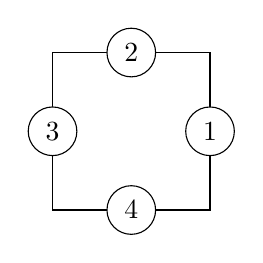
\begin{tikzpicture}
      \draw (0,0) rectangle (2,2);
      \node[draw, fill=white, circle] at (1,2) {2}; % top
      \node[draw, fill=white, circle] at (1,0) {4}; % bottom
      \node[draw, fill=white, circle] at (0,1) {3}; % left
      \node[draw, fill=white, circle] at (2,1) {1}; % right
      % \node[draw, rotate=0] at (1,1) {$D_8$}; % right
    \end{tikzpicture}
    ~
    \begin{tikzpicture}
      \draw (0,0) rectangle (2,2);
      \node[fill=white, circle] at (1,2) {3}; % top
      \node[fill=white, circle] at (1,0) {1}; % bottom
      \node[fill=white, circle] at (0,1) {4}; % left
      \node[fill=white, circle] at (2,1) {2}; % right
      % \node[draw, rotate=270] at (1,1) {$D_8$}; % right
    \end{tikzpicture}
    ~
    \begin{tikzpicture}
      \draw (0,0) rectangle (2,2);
      \node[fill=white, circle] at (1,2) {4}; % top
      \node[fill=white, circle] at (1,0) {2}; % bottom
      \node[fill=white, circle] at (0,1) {1}; % left
      \node[fill=white, circle] at (2,1) {3}; % right
      % \node[draw, rotate=180] at (1,1) {$D_8$}; % right
    \end{tikzpicture}
    ~
    \begin{tikzpicture}
      \draw (0,0) rectangle (2,2);
      \node[fill=white, circle] at (1,2) {1}; % top
      \node[fill=white, circle] at (1,0) {3}; % bottom
      \node[fill=white, circle] at (0,1) {2}; % left
      \node[fill=white, circle] at (2,1) {4}; % right
      % \node[draw, rotate=90] at (1,1) {$D_8$}; % right
    \end{tikzpicture}

    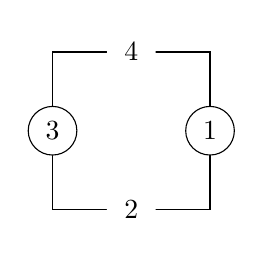
\begin{tikzpicture}
      \draw (0,0) rectangle (2,2);
      \node[fill=white, circle] at (1,0) {2}; % bottom
      \node[fill=white, circle] at (1,2) {4}; % top
      \node[draw, fill=white, circle] at (0,1) {3}; % left
      \node[draw, fill=white, circle] at (2,1) {1}; % right
      % \node[draw, yscale=-1] at (1,1) {$D_8$}; % right

    \end{tikzpicture}
    ~
    \begin{tikzpicture}
      \draw (0,0) rectangle (2,2);
      \node[fill=white, circle] at (1,0) {3}; % bottom
      \node[fill=white, circle] at (1,2) {1}; % top
      \node[fill=white, circle] at (0,1) {4}; % left
      \node[fill=white, circle] at (2,1) {2}; % right
      % \node[draw, yscale=-1, rotate=270] at (1,1) {$D_8$}; % right
    \end{tikzpicture}
    ~
    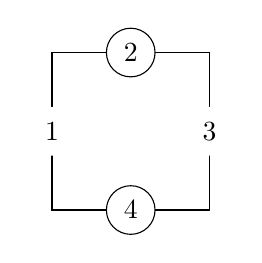
\begin{tikzpicture}
      \draw (0,0) rectangle (2,2);
      \node[draw, fill=white, circle] at (1,0) {4}; % bottom
      \node[draw, fill=white, circle] at (1,2) {2}; % top
      \node[fill=white, circle] at (0,1) {1}; % left
      \node[fill=white, circle] at (2,1) {3}; % right
      % \node[draw, yscale=-1, rotate=180] at (1,1) {$D_8$}; % right
    \end{tikzpicture}
    ~
    \begin{tikzpicture}
      \draw (0,0) rectangle (2,2);
      \node[fill=white, circle] at (1,0) {1}; % bottom
      \node[fill=white, circle] at (1,2) {3}; % top
      \node[fill=white, circle] at (0,1) {2}; % left
      \node[fill=white, circle] at (2,1) {4}; % right
      % \node[draw, yscale=-1, rotate=90] at (1,1) {$D_8$}; % right
    \end{tikzpicture}
    \caption[Facet derangements of a square.]{
      The $2^{2}2! = 8$ symmetries of a square with fixed sides circled.
      The square ($2$-dimensional hypercube) has symmetry group
      $S(2,2) = (\mathbb{Z}/2\mathbb{Z}) \wr \mathbb S_2$ and $D(2,2) = 5$ of these
      symmetries are derangements, meaning that they do not fix any sides.
    }
    \label{fig:squareDerangements}
  \end{figure}
\end{example}

While Theorem \ref{firstTheorem} gave us our first way to efficiently compute
the expected value of the first letter of a permutation on $kn$ letters with
a given number of $k$-cycles, we can also compute this efficiently with
Theorem \ref{secondTheorem} by using the formulas for $D(k,n)$ in Theorem \ref{derangementEGF}.
But this is not the only reason that Theorem \ref{secondTheorem} is of interest;
because of the structure of the formula it provides, this theorem suggests other
quantitative and qualitative insights.

Recall that when there are no restrictions on a permutation $\pi \in S_{kn}$, the
first letter is equally likely to take on any value,
so $\mathbb{E}[\pi(1) \mid \pi \in S_{kn}] = (kn+1)/2$.
% Recall also Proposition \ref{allSame},
% which stated that for $a \neq 1 \neq b$, there are the number of permutations with
% $m$ $k$-cycles starting with $a$ as there are starting with $b$.
The first insight given by Theorem \ref{secondTheorem}
is that the expected value of $\pi(1)$ with a given
number of $k$-cycles differs from $(kn+1)/2$ by at most $1/2$,
because $D(k,N) \geq 1$ for all $N \geq 0$ and $k \geq 2$.
%
Secondly, since $D(k, N)$ increases as a function of $N$, the expected value
gets closer to $(kn+1)/2$ as the number of $k$-cycles decreases.
%
Lastly, the numerator of $(-1)^{n-m}$ in the second summand of
Equation \eqref{eq:main} shows that the expected value of the first letter is
larger than $(kn+1)/2$ if and only if $n$ and $m$ have the same parity.
% Together, Corollary \ref{cor:kNotDivideN} and Theorem \ref{secondTheorem} fully
% explain both the even- and odd-indexed rows in the table in
% Table \ref{table:twoCycles}. Corollary \ref{cor:kNotDivideN} states that if
% $k \nmid n$, then $\pi(1)$ is equally likely to be any value between $1$ and $n$;
% Theorem \ref{secondTheorem} states that when $k \mid n$, then $\pi(1)$ is
% slightly more or less likely to be $1$, in an amount that relates to the number
% of derangements of a generalized symmetric group.

\section{A \texorpdfstring{$k$}{k}-cycle preserving bijection}
\label{section:bijection}
Motivated by Equation \eqref{eq:bijectionDifference0}, this section describes a
family of bijections,
  \begin{equation}\phi_k \colon S_{n-1} \times [n] \rightarrow S_n,\end{equation}
each of which preserves the number of $k$-cycles when $k \nmid n$.
Of course, there is no map that preserves the number of $k$-cycles when $k \mid n$. For example, a permutation in
$S_n$ consisting entirely of $k$-cycles contains $n/k$ $k$-cycles, while a permutation
in $S_{n-1}$ can contain at most $n/k - 1$ $k$-cycles by the pigeonhole principle.

% \begin{definition}
%   Given a word $\alpha = \alpha_1\alpha_2 \dots \alpha_n$ consisting of $n$
%   distinct letters in $\mathbb{N}_{>0}$, and a positive integer
%   $x \in \mathbb{N}_{>0}$, a \textbf{normalization} of the pair $(x,\alpha)$ is
%   a relabeling of the letters to be $[n+1]$, with each number appearing once,
%   where $\alpha$ keeps the same relative order.
% \end{definition}
% \begin{example}
%   The normalization of $(3,1398)$ is $\operatorname{normalize}(3,1376) = (2, 1354)$.
% \end{example}

Informally, these maps are defined by writing down a permutation $\sigma \in S_{n-1}$ in
\emph{canonical cycle notation}, incrementing all letters in $\sigma$
that are greater than or equal to $x \in [n]$,
inserting $x$ into the rightmost cycle, and then recursively moving letters into or out of subsequent cycles,
whenever a $k$-cycle is turned into a $(k+1)$-cycle or a $(k-1)$-cycle is
turned into a $k$-cycle.

\subsection{Example of recursive structure}

The definition of the map can look complicated, so it's worthwhile to start with
an example to give some sense of the overarching idea.

\begin{example}
  This example illustrates how the map $\phi_3$ inserts a letter into
  a permutation while preserving the
  number of $3$-cycles.
  The maps $\phi_k$ and $\psi_k$ are the result of moving letters according
  to the arrows and are applied from right to left.
  (This example uses the convention that $1 < 2 < \dots < 9 < A < B < \dots < N$.)

  ~
  \begin{align*}
    &\phi_3(
      (D         7          6)
      (E                                          \nS{eEnd})
      (F         \nW{3}{3}  2                     \nS{2End})
      (G         \nW{9}{9}  1          \nW{C}{C})
      (K \nS{k5} 5          \nW{4}{4})
      (L \nS{lj} J          \nW{8}{8})
      (M \nS{mb} B                                \nS{bEnd})
      (N         \nW{A}{A}  H                     \nS{hEnd})
      ,
      \nW{I}{I}
    ) \\
    &\hspace{1cm} = (D76)(E3)(F29)(G1)(KC5)(L4J)(M8BA)(NHI)
  \begin{tikzpicture}[remember picture,overlay]
    \draw[thick, ->]  (I) to[out=90, in=90, looseness=3.4] node[midway, above]{$\phi_3$} (hEnd);
    \draw[thick, ->]  (A) to[out=90, in=90, looseness=2] node[midway, above]{$\phi_3$} (bEnd);
    \draw[thick, ->]  (8) to[out=90, in=90, looseness=2] node[midway, above]{$\psi_3$} (mb);
    \draw[thick, ->]  (4) to[out=90, in=90, looseness=2] node[midway, above]{$\psi_3$} (lj);
    \draw[thick, ->]  (C) to[out=90, in=90, looseness=2] node[midway, above]{$\psi_3$} (k5);
    \draw[thick, ->]  (9) to[out=90, in=90, looseness=2] node[midway, above]{$\phi_3$} (2End);
    \draw[thick, ->]  (3) to[out=90, in=90, looseness=2] node[midway, above]{$\phi_3$} (eEnd);
  \end{tikzpicture}%
  \end{align*}

  \begin{align*}
    &\psi_3(
      (D         7         6)
      (E                   \nW{3}{3})
      (F \nS{f2} 2         \nW{9}{9})
      (G \nS{g1} 1                             \nS{1End})
      (K         \nW{C}{C} 5                   \nS{5End})
      (L         \nW{4}{4} J                   \nS{jEnd})
      (M         \nW{8}{8} B         \nW{A}{A})
      (N \nS{nh} H         \nW{I}{I})
    )\nS{outside}\\
    &\hspace{1cm} = ((D76)(E)(F32)(G91C)(K54)(LJ8)(MB)(NAH),I)
  \begin{tikzpicture}[remember picture,overlay]
    \draw[thick, ->]  (3) to[out=90, in=90, looseness=2] node[midway, above]{$\psi_3$} (f2);
    \draw[thick, ->]  (9) to[out=90, in=90, looseness=2] node[midway, above]{$\psi_3$} (g1);
    \draw[thick, ->]  (C) to[out=90, in=90, looseness=2] node[midway, above]{$\phi_3$} (1End);
    \draw[thick, ->]  (4) to[out=90, in=90, looseness=2] node[midway, above]{$\phi_3$} (5End);
    \draw[thick, ->]  (8) to[out=90, in=90, looseness=2] node[midway, above]{$\phi_3$} (jEnd);
    \draw[thick, ->]  (A) to[out=90, in=90, looseness=2] node[midway, above]{$\psi_3$} (nh);
    \draw[thick, ->]  (I) to[out=90, in=90, looseness=3.4] node[midway, above]{$\psi_3$} (outside);
  \end{tikzpicture}
  \end{align*}

\end{example}
Again, it is worth reemphasizing that the following definitions will follow the
convention that permutations are written in canonical cycle notation, \begin{equation}
  \pi =
    \underbrace{(c^{(t)}_1\cdots c^{(t)}_{\ell_t})}_{c^{(t)}}
    \cdots
    \underbrace{(c^{(1)}_1\cdots c^{(1)}_{\ell_1})}_{c^{(1)}},
\end{equation} where cycle $c^{(i)} = (c^{(i)}_1 \cdots c^{(i)}_{\ell_i})$ has $\ell_i$ letters.
This means that the first letter in each cycle, $c^{(i)}_1$, is the largest letter in that cycle,
and that the cycles are ordered in decreasing order by first letter when read from right to left:
$c^{(i+1)}_1 < c^{(i)}_1$ for all $i$.
\subsection{Formal definition and properties}
We will start by defining two functions, $\phi_k$ and $\psi_k$ which allow us
to insert a letter and extract a letter respectively. We will later see in
Lemma \ref{lem:bijection} that these functions are inverse to each other.
\begin{definition}
  Let $\phi_k \colon S_{n-1} \times [n] \rightarrow S_{n}$ be defined recursively as
  follows:
  \begin{equation}
    \phi_k(\emptyset, 1) = (1),
  \end{equation}
  and for $n>1$, $\pi \in S_{n-1}$, and $x \in [n]$,
  \begin{numcases}{\phi_k(\pi, x) =}
    \label{eq:phi_a}
    c^{(t)} \cdots c^{(1)}(x)                                                           & $x > c^{(1)}_1$            \\[10pt]
    \label{eq:phi_b}
    \phi_k(c^{(t)} \cdots c^{(2)}, c^{(1)}_2)(c^{(1)}_1 c^{(1)}_3 \cdots c^{(1)}_{k} x) & $\ell_1 = k$               \\[10pt]
    \label{eq:phi_c}
    \pi' (c^{(1)}_1 x' c^{(1)}_2\cdots c^{(1)}_{k-1} x)                                 & $\ell_1 = k-1, t > 1$ \\[10pt]
    \label{eq:phi_d}
    c^{(t)} \cdots c^{(2)} (c^{(1)}_1 \cdots c^{(1)}_{\ell_1} x)                        & otherwise.
  \end{numcases}
  Here, $\phi_k$ depends on the auxillary function
  $\psi_k \colon S_{n} \rightarrow S_{n-1} \times [n]$,
  \begin{numcases}{\psi_k(\pi) =}
    \label{eq:psi_a}
    \left(c^{(t)} \dots c^{(2)}, c^{(1)}_1\right)                                                              & $\ell_1 = 1$             \\[10pt]
    \label{eq:psi_b}
    \left(\phi_k(c^{(t)} \cdots c^{(2)}, c^{(1)}_2)(c^{(1)}_1 c^{(1)}_3 \dots c^{(1)}_k), c^{(1)}_{k+1}\right) & $\ell_1 = k + 1$         \\[10pt]
    \label{eq:psi_c}
    \left(\pi'(c^{(1)}_1 x' c^{(1)}_2 \dots c^{(1)}_{k-1}), c^{(1)}_k\right)                                   & $\ell_1 = k, t > 1$ \\[10pt]
    \label{eq:psi_d}
    \left(c^{(t)} \cdots c^{(2)}(c^{(1)}_1\cdots c^{(1)}_{\ell_1-1}),c^{(1)}_{\ell_1}\right)                   & otherwise,
  \end{numcases}
  and in both functions, $(\pi', x') = \psi(c^{(t)}\cdots c^{(2)})$.
\end{definition}

\begin{note}
  Strictly speaking, $\phi_k$ and $\psi_k$ have an additional implicit
  parameter $n$, which indicates the size of permutation that these functions
  act on. Since the constructions of these functions do not depend on $n$, this
  is suppressed in the notation.
\end{note}
The following theorem motivates this map,
and together with Lemma \ref{lem:bijection}, it implies Equation \eqref{eq:bijectionDifference0}.
\begin{theorem}
  If $k \nmid n$, the number of $k$-cycles of $\pi \in S_{n-1}$ is equal to the number of $k$-cycles in
  $\phi_k(\pi,x)$.
\end{theorem}
\begin{proof}
  By construction, the maps $\phi_k$ and $\psi_k$ change the rightmost cycle
  into a (different) $k$-cycle if it was previously a $k$-cycle, and they
  change non-$k$-cycles into non-$k$-cycles, except for the case where there is
  one cycle remaining with length $k-1$ (in the case of $\phi$) or length $k$
  (in the case of $\psi$). These cases can only be achieved when $k \mid n$, by
  the following lemma.
\end{proof}
\begin{lemma}
  The number of letters in $\pi$ in (recursive) applications of $\phi_k$ and
  $\psi_k$ are congruent to $n - 1\ (\mathrm{mod}\ k)$ and $n\ (\mathrm{mod}\ k)$,
  respectively.
  Therefore, the only time that the input to $\phi_k$ can be a single cycle of
  length $k-1$ or the input to $\psi_k$ can be a single cycle of length $k$ is
  when ${n \equiv 0\ (\mathrm{mod}\ k)}$.
\end{lemma}
\begin{proof}
  The proof proceeds by induction on the number of recursive iterations of
  $\phi_k$ and $\psi_k$. The base case is clear: on the first application
  of the map
  $\phi_k \colon S_{n-1} \times [n] \rightarrow S_n$, the input permutation
  has $n-1$ letters by definition.

  Now, either we're finished, or we recurse
  (Equations \eqref{eq:phi_b}, \eqref{eq:phi_c}, \eqref{eq:psi_b}, or \eqref{eq:psi_c}),
  which we look at case-by-case.
  \begin{enumerate}[leftmargin=*, label={\textbf{Case \arabic*.}}]
    \item In Equation \eqref{eq:phi_b}, the map $\phi_k$ sets aside $k$ letters from the input, so the number of letters in the recursive input to $\phi_k$ is also congruent to $n - 1 \ (\mathrm{mod}\ k)$.
    \item In Equation \eqref{eq:phi_c}, the map $\phi_k$ sets aside $k - 1$ letters from the leftmost cycle of the input. Since the number of letters in the original permutation was congruent to $n-1 \ (\mathrm{mod}\ k)$, the number of letters in the permutation being input to $\psi_k$ is congruent to $n   \ (\mathrm{mod}\ k)$.
    \item In Equation \eqref{eq:psi_b}, the map $\psi_k$ sets aside $k + 1$ letters from the leftmost cycle of the input. Since the number of letters in the original permutation was congruent to $n   \ (\mathrm{mod}\ k)$, the number of letters in the permutation being input to $\phi_k$ is congruent to $n-1 \ (\mathrm{mod}\ k)$.
    \item In Equation \eqref{eq:psi_c}, the map $\psi_k$ sets aside $k$ letters from the input, so the number of letters in the recursive input to $\psi_k$ is also congruent to $n \ (\mathrm{mod}\ k)$.
  \end{enumerate}
\end{proof}
The following lemma provides a certain ``niceness'' property of the map,
which allows us to analyze it. In particular, all recursive inputs in both
$\phi_k$ and $\psi_k$ are written in canonical cycle notation.
\begin{lemma}
  The output of $\phi_k$ is in canonical cycle notation.
\end{lemma}
\begin{proof}
  % 2DO: Strictly speaking, this should be an inductive argument similar to
  % the previous.
  Canonical cycle notation is preserved by construction.
  In particular, $\phi_k$ moves the first letter in any cycle, and
  Equation \eqref{eq:phi_a} guards against inserting a number into a cycle that
  is bigger than the largest number already in the cycle.
  Similarly, $\psi_k$ only moves the first letter in the case of Equation
  \eqref{eq:psi_a}, but in this case, the cycle only has one letter, so this is
  equivalent to deleting the cycle.
\end{proof}
\subsection{Inverting the bijection}
\begin{lemma}
  \label{lem:bijection}
  The maps
  $\phi_k \colon S_{n-1} \times [n] \rightarrow S_n$ and
  $\psi_k \colon S_n \rightarrow S_{n-1} \times [n]$ are inverse to one another.
\end{lemma}
\begin{proof}
  To prove this lemma, it suffices to show that $\psi_k \circ \phi_k = \operatorname{id}$
  by induction on the number of cycles of $\pi$. This will simultaneously prove
  that $\phi_k \circ \psi_k = \operatorname{id}$, because $S_{n-1} \times [n]$
  and $S_n$, both having $n!$ elements, have the same cardinality.

  When $\pi$ has no cycles, the base case is clear:
  $\psi_k(\phi_k(\emptyset, x)) = \psi_k((x)) = (\emptyset, x)$.

  Now there are five remaining cases to check, corresponding to each of the
  cases in the definition of $\phi_k(\pi, x)$:
   \begin{enumerate}[leftmargin=*, label={\textbf{Case \arabic*.}}]
    \item Assume $x > c_1^{(1)}$, so that $\phi_k(\pi,x)$ is evaluated via Equation \eqref{eq:phi_a}: \begin{align}
      \psi_k(\phi_k(\pi, x))
      &= \psi_k(c^{(t)}\cdots c^{(1)}(x)) \\
      &= (c^{(t)}\cdots c^{(1)},x) \\
      &= (\pi, x).
    \end{align}
    \item Assume $\ell_1 = k$, so that $\phi_k(\pi,x)$ is evaluated via Equation \eqref{eq:phi_b}:\begin{align}
      \psi_k(\phi_k(\pi, x))
      &= \psi_k(\phi_k(c^{(t)} \cdots c^{(2)}, c^{(1)}_2)
      \underbrace{
        (c^{(1)}_1 c^{(1)}_3 \cdots c^{(1)}_{k} x)
      }_{\text{length } k}) \\
      &= (\pi'(c^{(1)}_1x'c^{(1)}_3 \dots c^{(1)}_k), x)
    \end{align}
    \item Assume $\ell_1 = k - 1$ and $t > 1$, so that $\phi_k(\pi,x)$ is evaluated via Equation \eqref{eq:phi_c}:  \begin{align}
      \psi_k(\phi_k(\pi, x))
      &= \psi_k(\pi'
        \underbrace{
          (c^{(1)}_1 x' c^{(1)}_2\cdots c^{(1)}_{k-1} x)
        }_{\text{length } k + 1}
      )
    \end{align} where $(\pi', x') = \psi_k(c^{(t)} \dots c^{(2)})$.
    Therefore, this simplifies by Equation \eqref{eq:psi_c}: \begin{align}
      \psi_k(\phi_k(\pi, x)) &= \left(
        \phi_k(\pi', x')
        (c^{(1)}_1 \cdots c^{(1)}_{k-1}),
        x
      \right) \\
      &= \Big(
        \underbrace{
          \phi_k(\psi_k(c^{(t)} \dots c^{(2)}))
        }_{c^{(t)} \dots c^{(2)}}
        \underbrace{
          (c^{(1)}_1 \cdots c^{(1)}_{k-1})
        }_{c^{(1)}},
        x
      \Big) \\
      &= (\pi, x),
    \end{align} because $\phi_k(\psi_k(c^{(t)} \dots c^{(2)})) = c^{(t)} \dots c^{(2)}$
    by the induction hypothesis on $t-1$ letters.
    \item Assume that $x > c_1^{(1)}$ and $\ell_1 \not\in \{k-1,k\}$, so that $\phi_k(\pi,x)$ is evaluated via Equation \eqref{eq:phi_d}: \begin{align}
      \psi_k(\phi_k(\pi, x))
      &= \psi_k(c^{(t)} \cdots c^{(2)} (c^{(1)}_1 \cdots c^{(1)}_{\ell_1} x)) \\
      &= (c^{(t)}\cdots c^{(1)},x) \\
      &= (\pi, x).
    \end{align}
    \item Assume that $\ell_1 = k-1$ and $t = 1$, so that $\phi_k(\pi,x)$ is evaluated via Equation \eqref{eq:phi_d}: \begin{align}
      \psi_k(\phi_k(\pi, x))
      &= \psi_k((c^{(1)}_1 \cdots c^{(1)}_{k-1  } x)) \\
      &= (c^{(1)},x) \\
      &= (\pi, x).
    \end{align}
  \end{enumerate}
\end{proof}
In this section we constructed a recursively defined map and its inverse to
give a bijective proof that $C_k(n,m) = nC_k(n-1,m)$ when $k \nmid n$. This
is a novel, reversible algorithm for inserting a letters into a permutation
that preserves the number of $k$-cycles whenever possible.
\section{Further directions}
\label{section:furtherDirections}
In the introduction, we mentioned Conger's paper which analyzed how the number
of descents of a permutation affects the expected value of the first letter
of the permutation.
And similarly in the following sections, we looked at how the number of $k$-cycles
affects the expected value of the first letter of the permutation.
This section will principally look at the obvious generalization: given some
permutation statistic $\operatorname{stat}\colon S_n \rightarrow \mathbb Z$,
does the map \begin{equation}
  f(n,m) = \mathbb E[\pi(i) \mid \pi \in S_n, \operatorname{stat}(\pi)=m]
\end{equation} have any interesting structure?

Notice that the first letter of a permutation is itself a statistic, so
we can ask a more general question. Given pairs of statistics
$(\operatorname{stat}_1, \operatorname{stat}_2)$, does the map
\begin{equation}
  g(n,m) = \mathbb E[\operatorname{stat}_1(\pi) \mid \pi \in S_n, \operatorname{stat}_2(\pi)=m]
\end{equation} have any interesting structure?

\subsection{FindStat database}
The result by Conger gives the expected value of $\pi(1)$ given
$\operatorname{des}(\pi)$, and this chapter gave the expected value of
$\pi(1)$ given the number of $k$-cycles of $\pi$. Of course, it would be
interesting to do analogous analysis with other statistics.
In particular,
the FindStat permutation statistics database \cite{FindStat} contains over
380 different permutation statistics, and many of these appear to have some
structure with respect to the expected value of the first letter of a
permutation.

Moreover, this database currently has a total of about $1800$ statistics on a
variety of combinatorial objects: binary trees, Dyck paths, parking functions,
posets, and standard tableaux, to name a few.
By choosing two statistics on a given object, it may be interesting to ask how
knowing the value of one statistic changes the expected value of the other.

\subsection{Mahonian statistics}
In particular, the family of Mahonian statistics may be fruitful to investigate.
Below, we have given conjectures about two: the major index and the inversion number.
Mahonian statistics are maps
$\operatorname{mah} \colon S_n \rightarrow \mathbb{N}_{\geq0}$ that are
equidistributed with the inversion number.\cite{Foata} That is, \begin{equation}
  \#\{w \in S_n : \operatorname{mah}(w) = k\} =
  \#\{w \in S_n : \operatorname{inv}(w) = k\}.
\end{equation}
Naturally, all Mahonian statistics share the same generating function: \begin{equation}
  \sum_{\sigma \in S_n} x^{\operatorname{mah}(\sigma)}
    = [n]_q!
    = \prod_{i=0}^{n-1}\sum_{j=0}^i(q^j).
\end{equation}

Because the expected value of the first letter is given by the weighted sum of
the permutations with $\operatorname{mah}(w) = k$ divided by the number of such
permutations, $\mathbb{E}[\pi(1)\, |\, \pi \in S_n, \operatorname{mah}(\pi) = k]$
has a denominator that is (a factor of) $M(n,k)$, the number of permutations
of $w \in S_n$ such that $\operatorname{inv}(w) = k$. For fixed $k$, these
satisfy a degree-$k$ polynomial for all $n > k$. Notably, in the cases of
the major index and the inversion number, the numerators appear to satisfy
degree-$k$ and {degree-$k-1$} polynomials respectively.

\begin{conjecture}
  For fixed $k$ and $n > k$, the expected value of the first letter of a
  permutation with a given number of inversions is equal to a rational function
  in $n$ given by \begin{equation}
    \mathbb{E}[\pi(1)\, |\, \pi \in S_n, \operatorname{inv}(\pi) = k]
    = \frac{M(n+1,k)}{M(n,k)},
  \end{equation} where $M(n,k)$, as above, is the number of permutations $w \in S_n$ such
  that $\operatorname{inv}(w) = k$.
\end{conjecture}

\begin{conjecture}
  For fixed $k > 0$ and $n \geq k$,
  $\mathbb{E}[\pi(1)\, |\, \pi \in S_n, \operatorname{maj}(\pi) = k]$
  satisfies a rational function in $n$ that is $1/(k+1)$ times the quotient of a monic
  degree-$(k+1)$ polynomial by a monic degree-$k$ polynomial. Specifically,

  \begin{align}
    \mathbb{E}[\pi(1)\, |\, \pi \in S_n, \operatorname{maj}(\pi) = 1] &= \frac{1}{2}\left(\frac{n^2 + n - 2}{n-1}\right),
    \\[2mm]
    \mathbb{E}[\pi(1)\, |\, \pi \in S_n, \operatorname{maj}(\pi) = 2] &= \frac{1}{3}\left(\frac{n^3 - n - 6}{n^2 - n - 2}\right),
    \\[2mm]
    \mathbb{E}[\pi(1)\, |\, \pi \in S_n, \operatorname{maj}(\pi) = 3] &= \frac{1}{4}\left(\frac{n^4 + 6 n^3 - 13 n^2 - 18 n}{n^3 - 7n}\right),
    \text{ and}
    \\[2mm]
    \mathbb{E}[\pi(1)\, |\, \pi \in S_n, \operatorname{maj}(\pi) = 4] &= \frac{1}{5}\left(\frac{n^5 + 20 n^4 - 45 n^3 - 80 n^2 - 16 n}{n^4 + 2 n^3 - 13 n^2 - 14 n}\right).
    % % \mathbb{E}[\pi(1)\, |\, \pi \in S_n, \operatorname{maj}(\pi) = 5] &= \frac{1}{6}\left(\frac{n^6 + 51 n^5 + 85 n^4 - 195 n^3 - 806 n^2 - 1296 n}{n^5 + 10 n^4 + 15 n^3 - 70 n^2 - 196 n}\right).
  \end{align}
  Note that the denominator is given by an integer multiple of $M(n,k)$,
  a degree-$k$ polynomial.
\end{conjecture}

\subsection{An elusive bijection}

  Let $F_k(n, m)$ be the number of elements of the generalized symmetric group
  $S(k,n) = (\mathbb{Z}/k\mathbb{Z}) \wr S_n$ with $m$ fixed points,
  and recall that $C_k(n,m)$ is the number of elements of $S_{kn}$ with $m$ $k$-cycles.
  For each pair of nonnegative integers $(\alpha, \beta)$
  with $\alpha, \beta \leq n$, Lemma \ref{lem:fixedPointsAndCycles} suggests that
  there exists a bijection of sets \begin{equation}
    C_k(n, \alpha) \times F_k(n, \beta) \rightarrow C_k(n, \beta) \times F_k(n, \alpha).
  \end{equation}
  This bijection has proven to be elusive to construct outside of the special
  cases where $n=1$ or $k=1$.
  Note that the map cannot be a group automorphism of $S_{kn} \times S(k,n)$,
  because the identity of this group is in $C_k(n,0) \times F_k(n,n)$, so it
  cannot be preserved under this map.

  It would be especially interesting if there's a way to use the embedding of
  $(\mathbb{Z}/k\mathbb{Z}) \wr S_n$ into $S_{kn}$ as the centralizer of an
  element that is the product of $n$ disjoint $k$-cycles.

\chapter{Unranking Restricted Permutations}
\label{cha:UnrankingMenage}
TODO

\section{TODO}
\begin{enumerate}
  \item Introduction
  \item Define \textbf{derived} complementary board $B_\alpha^c$?
  \item If we do a cyclic rotation of the rows of a chessboard, we get
    essentially the same thing.
  \item Move code to Appendix.
  \item Define $B_\alpha$ and $\overline{B}_\alpha^c$.
  \item Do we want to talk about parking functions?
  \item Is it worthwhile to discuss prefix functions for compositions, etc.?
  \item Make sure ``derank'' doesn't occur anywhere.
  \item Gives a way of sampling uniformly at random.
\end{enumerate}

% %%%%%%%%%%%%%%%%%%%%%%%%%%%%%%%%%%%%%%%%%%%%%
% Section 1
% %%%%%%%%%%%%%%%%%%%%%%%%%%%%%%%%%%%%%%%%%%%%%
\section{Overview and History}

In January 2020, Richard Arratia sent out an email announcing a talk he was
going to give on de-ranking derangements.

By January 2021, he announced a \$100 prize for solving the analogous problem
with m\'enage permutations. I solved that too.

Richard was interested in a more general question, which I found contagious:
Given some family of combinatorial objects that can be quickly counted
(say unlabelled simple graphs on $n$ vertices)
and some total ordering on them,
when is it possible to \textbf{unrank} the collection in some computationally
efficient way?

\begin{definition}
  Let $\mathcal C$ be a totally ordered finite set, and
  let $\{c_i\}_{i=1}^{|\mathcal C|}$ be the unique sequence of elements in
  $\mathcal{C}$ such that $c_i < c_{i+1}$ for all $1 \leq i < |\mathcal{C}|$.

  The \textbf{ranking map} is the map
  $\operatorname{rank}_{\mathcal{C}} \colon \mathcal{C} \rightarrow \mathbb N_{>0}$
  which sends $c_i \mapsto i$.

  The \textbf{unranking map} is the inverse map
  $\operatorname{unrank}_{\mathcal{C}} \colon \mathbb N_{>0} \rightarrow \mathcal{C}$
  which sends $i \mapsto c_i$.
\end{definition}

In abstract terms, these maps are not particularly interesting, but in practical
terms it can be quite difficult to efficiently compute a given ranking or
unranking from a given totally ordered set. After all, when these sets
grow in exponential time or worse, explicitly constructing the sequence and
doing a search is not computationally feasible.

In Appendix TODO, we will provide examples of total orders on combinatorial
objects $\mathcal{C}$ for which constructing efficient

% Of course, we can usually create an algorithm to give the $i$-th object without
% simply enumerating all of the objects explicitly? We want to ``jump in'' to a
% specific place on the list. Another interesting question:
% what if you get to supply both the total order and the unranking algorithm?

In this chapter we're going to explore that idea. We're going to show a general
theory that allows us to de-rank
permutations in lexicographic order,
derangements in lexicographic order,
partitions and compositions of $n$ in lexicographic order,
labeled trees by lexicographic order of Pr\"ufer code,
Lyndon words \cite{Kociumaka2014} (de Bruijn Sequences?),
Dyck path in lexicographic order?
% %%%%%%%%%%%%%%%%%%%%%%%%%%%%%%%%%%%%%%%%%%%%%
% Section 2
% %%%%%%%%%%%%%%%%%%%%%%%%%%%%%%%%%%%%%%%%%%%%%
\section{Prefix Counting and Word Ranking}

% If we can efficiently count how many objects in
% $[n]^k$ start with a given prefix
% (in $O(T(n,k))$ time),
% then we can just walk down the possible letters until
% we get to the right spot ($O(nkT(n,k))$).

\begin{lemma}
  If we have
  an efficient way to compute the unranking map,
  an efficient way to compare two elements in the total order,
  and an efficient way of computing the number of objects at hand, $|\mathcal C|$,
  then we can efficiently compute the ranking map.
  \label{lemma:unrankToRank}
\end{lemma}
\begin{proof}
  We can do a binary search. (TODO: write pseudo-code algorithm?)
\end{proof}

\subsection{Counting Words With a Given Prefix}
In both the case of unranking derangements and menage permutations
(and in many other applications) our combinatorial objects are
words and our total order is lexicographic order.

\begin{definition}
  \textbf{Lexicographic order} is a total ordering on words where $w < v$ ... TODO
\end{definition}

\begin{definition}
  A finite \textbf{word} $w$ over an alphabet $\mathcal A$ is a finite sequence
  $\{w_i \in \mathcal A\}_{i=1}^N$.

  The collection of finite words over the alphabet $\mathcal A$ is denoted by
  $\mathcal{W}_\mathcal{A}$, or just $\mathcal{W}$ when the alphabet is
  implicit from context.
\end{definition}

\begin{definition}
  A word $w = \{w_i \in \mathcal A\}_{i=1}^N$ is said to begin with a
  \textbf{prefix} $\alpha = \{\alpha_i \in \mathcal A\}_{i=1}^M$ if
  $M \leq N$ and $w_i = \alpha_i$ for all $i \leq M$.
\end{definition}

\begin{lemma}
  Let $\mathcal{W}$ be the set of words of any length on the alphabet $[n]$,
  and let $\mathcal C \subsetneq \mathcal{W}$ be a finite subset of words
  on this alphabet, with a total order equal to its lexicographic order.

  Then let
  $\#\operatorname{prefix}_{\mathcal C}\colon \mathcal{W} \rightarrow \mathcal{C}$
  be the function that counts the number of words in $\mathcal C$ that begin
  with a given prefix.

  Then the unranking function can be computed recursively by \[
    \operatorname{unrank}_\mathcal{C}(i) = f^{\mathcal C}_i((1), 0)
  \] where
  \begin{equation}
  f^{\mathcal C}_i(\alpha, j) = \begin{cases}
    \alpha
      & i \in (j, j + \#\operatorname{prefix}_\mathcal{C}(\alpha)] \text{ and } \alpha \in \mathcal{C} \\
    f^{\mathcal C}_i(\alpha', j)
      & i \in (j, j + \#\operatorname{prefix}_\mathcal{C}(\alpha)] \text{ and } \alpha \not\in \mathcal{C} \\
    f^{\mathcal C}_i(\alpha'', j + \#\operatorname{prefix}_\mathcal{C}(\alpha))
      & \text{otherwise},
  \end{cases}
\end{equation}
where
$\alpha = (\alpha_1, \alpha_2, \dots, \alpha_\ell)$,
$\alpha' = (\alpha_1, \alpha_2, \dots, \alpha_\ell, 1)$,
$\alpha'' = (\alpha_1, \alpha_2, \dots, \alpha_{\ell-1}, 1 + \alpha_\ell)$,
and $j$ denotes the number of words in $\mathcal{C}$ that occur strictly
before $\alpha$.
\end{lemma}
\begin{proof}
  TODO (sketch)
  The second line appends a letter, which can happen at most $n$ times.
  The third line increments the last letter, which can happen at most $k$ times
  per position.
\end{proof}

This shows that if we can construct a function
$\#\operatorname{prefix}_\mathcal{C}$ that efficiently counts the number of
elements of $\mathcal{C}$ with a given prefix, then we can efficiently rank and
unrank the elements of $\mathcal{C}$ in lexicographic order.
% This technique works when we can write our objects as a word in $[n]^k$, and
% we order the objects
% by the lexicographic order of the words. In the case that our objects cannot be
% written as words, or we are interested in an order other than lexicographic order,
% a different technique must be used.

\subsection{Ranking words}
In Lemma \ref{lemma:unrankToRank}, we showed that given an efficient algorithm
to compute $\operatorname{unrank}_\mathcal{C}$, we can derive an efficient
algorithm to compute $\operatorname{rank}_\mathcal{C}$, on the order of
$O(\log(|\mathcal{C}|\operatorname{unrank}_\mathcal{C}(n)))$
(TODO: make the size of the input explicit.)

However, we can provide a faster algorithm via another recursive function:
$\operatorname{rank}_\mathcal{C}(w) = g_w(1,1,0)$ where
\begin{equation}
  g_w(i, \ell, c) = \begin{cases}
    c + 1 & \ell = w_i \text{ and } i = |w| \\
    g_w(i + 1, 1, c) & \ell = w_i \text{ and } i < |w| \\
    g_w(i, \ell + 1, c + \#\operatorname{prefix}_\mathcal{C}(w')) & \ell < w_i,
  \end{cases}
\end{equation}
where $w' = (w_1, w_2, \dots, w_{i-1}, \ell)$.

\section{Basic Notions of Rook Theory}
Because we have showed that we can ... TODO
In the case of unranking derangements and permutations, it is useful to use
ideas from rook theory, which provides a theory for understanding
position-restricted permutations.
Rook Theory was introduced by Kaplansky and Riordan \cite{Kaplansky1946}
in their 1946 paper \textit{The Problem of the Rooks and its Applications}. In
it, they discuss problems of restricted permutations in the language of rooks
placed on a chessboard.

\begin{figure}[h]
  \center
  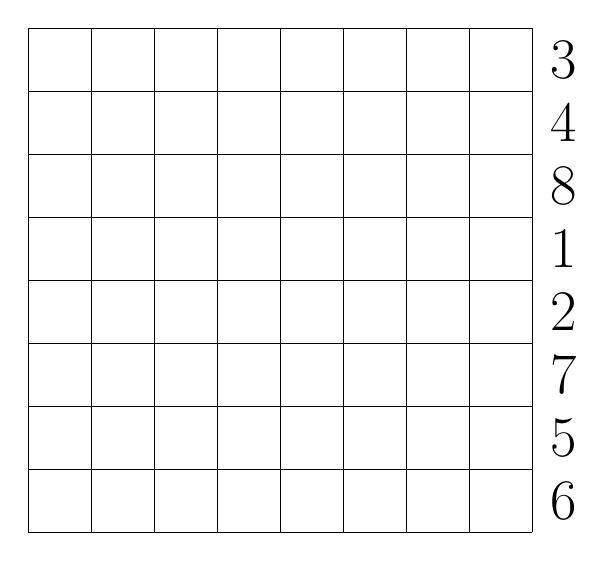
\begin{tikzpicture}[scale = 0.8]
    \foreach \i/\j in {1/3,2/4,3/8,4/1,5/2,6/7,7/5,8/6} {
      \node at (\j - 0.5, 8.5 - \i) {\huge\rook};
      \node at (8.5, 8.5-\i) {\huge\j};
    }
    \draw (0,0) grid (8,8);
  \end{tikzpicture}
  \caption[A permutation corresponding to a rook placement.]{
    An illustration of the rook placement corresponding to the permutation
    $34812756 \in S_8$. A rook is placed in square $(i, \pi(i))$ for each $i$.
  }
  \label{fig:permutationFromRooks}
\end{figure}


\subsection{Definitions in rook theory}
We begin by introducing some preliminary ideas from rook theory.

\begin{definition}
  A \textit{board} $B$ is a subset of $[n] \times [n]$ which represents the
  squares of a $n \times n$ chessboard that rooks are allowed to be placed on.
  Every board $B$ has a \textit{complementary board}
  $B^c = ([n] \times [n]) \setminus B$, which consists of all of the
  squares of $B$ that a rook cannot be placed on.
\end{definition}

To each board, we can associate a generating polynomial that keeps track of the
number of ways to place a given number of rooks on the valid squares in such a
way that no two rooks are in the same row or column.

\begin{definition}
  The \textit{rook polynomial} associated with a board $B$,
  \[
    p_B(x) = r_0 + r_1 x + r_2 x^2 + \dots + r_n x^n,
  \]
  is a generating polynomial where $r_k$ denotes the number of $k$-element subsets
  of $B$ such that no two elements share an $x$-coordinate or a $y$-coordinate.
\end{definition}

In the context of permutations, we're typically interested in $r_n$, the number
of ways to place $n$ rooks on a restricted $n \times n$ board.
However, it turns out that a naive application of the techniques from
rook theory do not immediately allow us to count the number of
restricted permutations with a given prefix.
Computing the number of such permutations is known to be computationally hard
for a board with arbitrary restrictions.
We can see this by encoding a board $B$ as a $(0,1)$-matrix and computing the matrix
permanent. (In fact, Shevelev \cite{Shevelev1992} claims that
``the theory of enumerating the permutations with restricted positions
stimulated the development of the theory of the permanent.'')

\begin{lemma}
  Let $M_B = \{a_{ij}\}$ be an $n \times n$ matrix where \[
    a_{ij} = \begin{cases}
      1 & (i,j) \in B \\
      0 & (i,j) \not\in B
    \end{cases}.
  \]
  Then the coefficient of $x^n$ in $p_B(x)$ is given by the matrix permanent
  \[
    \operatorname{perm}(M_B) = \sum_{\sigma \in S_n} \prod_{i=1}^n a_{i\sigma(i)}.
  \]
\end{lemma}

Now is an appropriate time to recall Valiant's Theorem.

\begin{theorem}[Valiant's Theorem \cite{Valiant1979}]
  Computing the permanent of a (0,1)-matrix is \#P-complete.
\end{theorem}

\begin{corollary}
  Computing the number of rook placements on an arbitrary $n \times n$ board is
  \#P-hard.
\end{corollary}

Therefore, in order to compute the number of permutations, we must exploit some
additional structure of the restrictions.

\subsection{Techniques of Rook Theory}
Rook polynomials can be computed recursively. The base case is that
for an empty board $B = \emptyset$, the corresponding rook polynomial is
$p_\emptyset(x) = 1$, because there is one way to place no rooks, and no way
to place one or more rooks.
\begin{lemma}[\cite{Riordan1980}]
  Given a board, $B$, then for any square $(x,y) \in B$, we can define
  the resulting boards if we include or exclude the square respectively
  \begin{align}
    B_i &= \{(x',y') \in B : x \neq x' \text{ and } y \neq y'\} \\
    B_e &= B \setminus {(x,y)}.
  \end{align}
  Then we can write the rook polynomial for $B$ in terms of this decomposition.
  \[
    p_B(x) = xp_{B_i}(x) + p_{B_e}(x).
  \]
  \label{lemma:rookPolynomialRecursion}
\end{lemma}

If we want to compute a rook polynomial using this construction, we can end
up adding up lots of smaller rook polynomials---a number that is exponential in
the size of $B$.
However, when the number of squares in $B^c$ is small in some sense, it can be
easier to compute the rook polynomial $p_{B^c}$ and use the principle of
inclusion/exclusion on it's coefficients to determine the rook polynomial for
the original board, $B$.

In the case of derangements and m\'enage permutations, this is the strategy
we'll use.
Start by finding the resulting board from a given prefix,
find the rook polynomial of the complementary board, and
use the principle of inclusion/exclusion to determine the number of ways to
place rooks in the resulting board.

\section{Unranking Derangements}

In January 2020, Richard Arratia sent out an email proposing a seminar talk.
The title describes the first ``\$100 problem'':
\begin{problem}
``For $100$ dollars, what is the $500$ quadrillion-th derangement on $n=20$?''
\end{problem}

\begin{answer}
The computer program in Appendix TODO computed the answer in less than ten
milliseconds. When written as words in lexicographic order, the
derangement in $S_{20}$ with rank $5 \times 10^{17}$ is \[
  12\ 14\ 2\ 9\ 13\ 20\ 6\ 3\ 1\ 17\ 5\ 11\ 19\ 15\ 10\ 18\ 8\ 7\ 4\ 16.
\]
\end{answer}

Arratia's question focused on unranking derangements where the rank was
based on the total ordering that comes from writing the
permutations as words in lexicographic order.
Other authors have looked at unranking derangements based on other total
orderings. In particular, Mikawa and Tanaka \cite{Mikawa2014} give an algorithm
to rank/unrank derangements
with respect to \textit{lexicographic ordering in cycle notation}.

In this section we will develop an algorithm for ranking and unranking with
respect to their lexicographic ordering as words. The technique that we use will
broadly be re-used in the next section.
It is worthwhile to begin by recalling the definition of a derangement.
\begin{definition}
  A \textit{derangement} is a permutation $\pi \in S_n$ such that $\pi$ has no
  fixed points. That is, the set of derangements is \[
    \{\pi \in S_n : \pi(i) \neq i\ \forall i \in [n]\}.
  \]
\end{definition}

\subsection{The complementary board.}
In order to compute the number of derangements with a given prefix, it is
useful to look at the board that results after placing $k$ rooks according to
these positions, as illustrated in Figure \ref{fig:derangementPrefix}.

\begin{figure}
  \center
  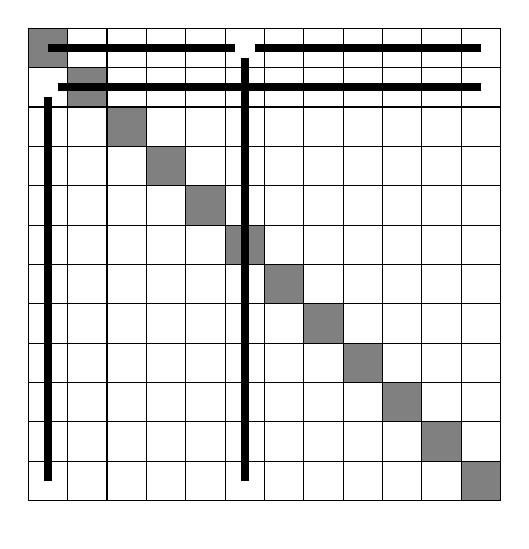
\begin{tikzpicture}[scale = 0.5]
    \path (0,-0.5) -- (0,6.5);
    \foreach \i in {0,...,11} { \fill[gray] (\i, 12-\i) rectangle (\i + 1, 11 - \i); }
    \draw (0,0) grid (12,12);
    \node (R1) at (5.5, 11.5) {\Large\symrook};
    \node (R2) at (0.5, 10.5) {\Large\symrook};
    \draw[line width = 3]
      (0.5,11.5) -- (R1) -- (11.5,11.5)
      (R1) -- (5.5,0.5)
    ;
    \draw[line width = 3]
      (R2) -- (11.5,10.5)
      (R2) -- (0.5,0.5)
    ;
  \end{tikzpicture}
  ~~
  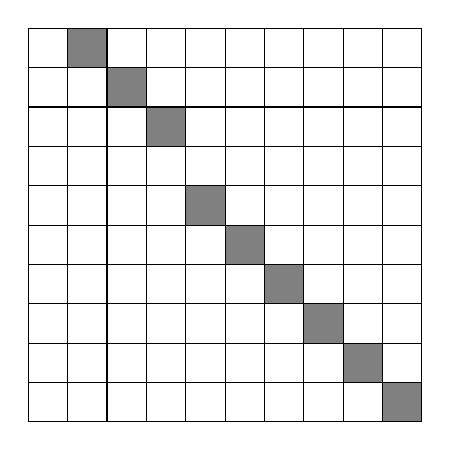
\begin{tikzpicture}[scale = 0.5]
    \path (0,-0.5) -- (0,6.5);
    \foreach \i in {1,...,3} { \fill[gray] (\i, 11-\i) rectangle (\i + 1, 10 - \i); }
    \foreach \i in {4,...,9} { \fill[gray] (\i, 10-\i) rectangle (\i + 1, 9 - \i); }
    \draw (0,0) grid (10,10);
  \end{tikzpicture}
  \caption[The derived board for a prefix of a derangement.]{An example of a prefix $\alpha = (6, 1)$, and the board that results
  from deleting the first $\ell = 2$ rows and columns $6$ and $1$.
  The derived complementary board of $B$ from $\alpha$ is
  $B^c_\alpha = \{(1,2), (2,3), (3,4), (5,5), \dots, (10,10)\}$.}
\label{fig:derangementPrefix}
\end{figure}


\begin{definition}
  If $B$ is an $n \times n$ board, and
  $\alpha = (\alpha_1, \alpha_2, \dots, \alpha_\ell)$ is a valid prefix of length
  $\ell$, then \textbf{derived complementary board} of $B$ from $\alpha$,
  denoted $B^c_\alpha$,
  is $B$ with the appropriate rows and columns removed and reindexed in such
  a way that $B^c_\alpha \subseteq [n - \ell] \times [n - \ell]$.
  % \[
  %   B^c_\alpha \cup \{(x, y) : x \in [n], y \in [\ell]\} \cup \{(x, y) : x \in \alpha, y \in [n]\}
  % \]
  % the \textit{derived complementary board} of $B$ from $\alpha$, denoted
  % $B^c_\alpha \subset [n-k]^2$ consisting of a subset of $B^c$, relabeled to
  % reflect ... TODO
\end{definition}
\begin{lemma}
  Given a valid $\ell$ letter prefix $(\alpha_1, \alpha_2, \dots, \alpha_\ell)$
  of a word on $n$ letters,
  the number of squares in the resulting complementary board is \[
    |B_\alpha^c| = n - \ell - |\{\ell+1, \ell+2, \dots, n\} \cap \{\alpha_1, \alpha_2, \dots, \alpha_\ell\}|,
  \] and no two of these squares are in the same row or column.
\end{lemma}
\begin{proof}
  TODO
  % Recall that $B^c = \{(1,1), (2,2), \dots, (n,n)\}$, so no square shares its
  % first or second coordinate with another square.
  % Because $B^c_\alpha$ is the result of deleting and relabeling the squares of
  % $B^c$, $B^c_\alpha$ also has two squares with with same first or second
  % coordinate.
  % In order to
  % Because the prefix is of length $\ell$, all of the squares in $B_\alpha^c$ must
  % have a first coordinate greater than $\ell$, that is,
  % $B_\alpha^c \subseteq \{(\ell+1, \ell+1), (\ell+2, \ell+2), \dots, (n, n)\}$.
  % Then, we can count how many of these remaining squares are in the same row or
  % column as a rook in the prefix. This number is the size of the intersection
  % $|\{\ell+1, \ell+2, \dots, N\} \cap \{\alpha_1, \alpha_2, \dots, \alpha_p\}|$.
\end{proof}

\subsection{Derangements with a given prefix}
Now that we have a way of quickly computing $|B_\alpha^c|$, we can compute the
number of ways to place $j$ rooks on the complementary board. We can use this
to compute the number of derangements that begin with the prefix $\alpha$.

\begin{lemma}
  The rook polynomial for the complementary board $B_\alpha^c$ is \begin{equation}
    p_{B_\alpha^c}(x) = \sum_{j = 0}^{|B_\alpha^c|} \binom{|B_\alpha^c|}{j}x^j.
  \end{equation}
\end{lemma}
\begin{proof}
  No two squares in $B^c$ (and thus $B^c_\alpha$) are in the same row or column.
  Thus the number of ways to place $j$ rooks is equivalent to selecting $j$
  cells from $|B^c_\alpha|$.
\end{proof}

Now we introduce a lemma of Stanley \cite{Stanley2011EC1} to compute the number
of TODO from a complementary board.

\begin{lemma}[\cite{Stanley2011EC1}]
  The number of ways, $N_0$, of placing $n$ nonattacking rooks on a board
  $B \subseteq [n] \times [n]$ is given by \[
    N_0 = \sum_{k=0}^n (-1)^k r_k (n-k)!,
  \] where $P_{B^c}(x) = \sum_{k=0}^n r_k x^k$.
  \label{lemma:CountsFromComplementaryPolynomials}
\end{lemma}

\begin{corollary}
  The number of derangements with prefix
  $\alpha = (\alpha_1, \alpha_2, \dots, \alpha_\ell)$
  is given by \[
    \#\operatorname{prefix}(\alpha)
    = \sum_{j=0}^{|B_\alpha^c|} (-1)^j \binom{|B_\alpha^c|}{j}(n-\ell-j)!,
  \] which is $\operatorname{A047920}(n-\ell, |B_\alpha^c|)$ in
  the On-Line Encyclopedia of Integer Sequences \cite{oeis}.
\end{corollary}

\begin{example}
  For example, for $N = 14$, we wish to count the number of derangements that
  start with the prefix $6\,1$. Since the prefix has two letters, $p = 2$ and
  $n = 14 - 2 = 12$. The only crossed-out cell that is deleted by the prefix in the
  remaining board is the cell that was in position $6$:
  in particular, $\{3,4,\dots,14\} \cap \{6, 1\} = 6$.
  Thus $k = 12 - 1 = 11$.
  Thus there are $A047920(12,11) = 190\,899\,411$ derangements that start
  with $6\,1$.
\end{example}
\begin{table}
\begin{tabular}{|l|r|l|c|l|}
  \hline
  $\alpha$ (prefix)   & $\operatorname{\#prefix}(\alpha)$ & index range & $|B_\alpha^c|$ & $f^{\mathcal{D}}_i(\alpha, \ell)$ \\
  \hline
  $1       $ & $0$    & $(0,0]$           & $-$ & $f^{\mathcal{D}}_{1000}(1, 0)$          \\
  $2       $ & $2119$ & $(0,2119]$        & $6$ & $f^{\mathcal{D}}_{1000}(2, 0)$          \\
  \hline
  $21      $ & $265$  & $(0, 265]$        & $6$ & $f^{\mathcal{D}}_{1000}(21, 0)$         \\
  $22      $ & $0$    & $(265, 265]$      & $-$ & $f^{\mathcal{D}}_{1000}(22, 265)$       \\
  $23      $ & $309$  & $(265, 574]$      & $5$ & $f^{\mathcal{D}}_{1000}(23, 265)$       \\
  $24      $ & $309$  & $(574, 883]$      & $5$ & $f^{\mathcal{D}}_{1000}(24, 574)$       \\
  $25      $ & $309$  & $(883, 1192]$     & $5$ & $f^{\mathcal{D}}_{1000}(25, 883)$       \\
  \hline
  $251     $ & $53$   & $(883, 936]$      & $4$ & $f^{\mathcal{D}}_{1000}(251, 883)$      \\
  $253     $ & $0$    & $(936, 936]$      & $-$ & $f^{\mathcal{D}}_{1000}(253, 936)$      \\
  $254     $ & $64$   & $(936, 1000]$     & $3$ & $f^{\mathcal{D}}_{1000}(254, 936)$      \\
  \hline
  $2541    $ & $11$   & $(936, 947]$      & $3$ & $f^{\mathcal{D}}_{1000}(2541, 936)$     \\
  $2543    $ & $11$   & $(947, 958]$      & $3$ & $f^{\mathcal{D}}_{1000}(2543, 947)$     \\
  $2546    $ & $14$   & $(958, 972]$      & $2$ & $f^{\mathcal{D}}_{1000}(2546, 958)$     \\
  $2547    $ & $14$   & $(972, 986]$      & $2$ & $f^{\mathcal{D}}_{1000}(2547, 972)$     \\
  $2548    $ & $14$   & $(986, 1000]$     & $2$ & $f^{\mathcal{D}}_{1000}(2548, 986)$     \\
  \hline
  $25481   $ & $3$    & $(986, 989]$      & $2$ & $f^{\mathcal{D}}_{1000}(25481, 986)$    \\
  $25483   $ & $3$    & $(989, 992]$      & $2$ & $f^{\mathcal{D}}_{1000}(25483, 989)$    \\
  $25486   $ & $4$    & $(992, 996]$      & $1$ & $f^{\mathcal{D}}_{1000}(25486, 992)$    \\
  $25487   $ & $4$    & $(996, 1000]$     & $1$ & $f^{\mathcal{D}}_{1000}(25487, 996)$    \\
  \hline
  $254871   $ & $2$   & $(996, 998]$      & $0$ & $f^{\mathcal{D}}_{1000}(254871, 996)$   \\
  $254873   $ & $2$   & $(998, 1000]$     & $0$ & $f^{\mathcal{D}}_{1000}(254873, 998)$   \\
  \hline
  $2548731  $ & $1$   & $(998, 999]$      & $0$ & $f^{\mathcal{D}}_{1000}(2548731, 998)$  \\
  $2548736  $ & $1$   & $(999, 1000]$     & $0$ & $f^{\mathcal{D}}_{1000}(2548736, 999)$  \\
  \hline
  $25487361 $ & $1$   & $(999, 1000]$     & $0$ & $f^{\mathcal{D}}_{1000}(25487361, 999)$ \\
  \hline
\end{tabular}
\caption[Steps for computing the $1000$th derangement in $S_8$]{
  There are $A000166(8) = 14833$ derangements on $8$ letters.
  This algorithm finds the derangement at index $1000$.
}
\end{table}

% %%%%%%%%%%%%%%%%%%%%%%%%%%%%%%%%%%%%%%%%%%%%%
% Section 3
% %%%%%%%%%%%%%%%%%%%%%%%%%%%%%%%%%%%%%%%%%%%%%
\section{Unranking M\'enage Permutations}

\subsection{Proof of concept (The \$100 answer!)}
In February 2020, Richard Arratia offered
\begin{problem}
  For $n=20$ there are $A000179(20) = 312\,400\,218\,671\,253\,762 > 3.1\cdot 10^{17}$
  m\'enage permutations.
  Determine the $10^{17}$-th such permutation when listed in lexicographic order.
\end{problem}
\begin{answer}
  The desired permutation is \begin{equation}
    7\ 16\ 19\ 12\ 2\ 8\ 15\ 1\ 18\ 14\ 3\ 9\ 20\ 10\ 5\ 17\ 13\ 4\ 11\ 6.
  \end{equation}
\end{answer}

A M\'enage permutation comes from the \textit{problème des ménages}. % https://en.wikipedia.org/wiki/M%C3%A9nage_problem
Here we will define it as
\begin{definition}
  A \textit{m\'enage permutation} is a permutation $\pi \in S_n$ such that for
  all $i \in [n]$,
  $\pi(i) \neq i$ and
  $\pi(i) + 1 \not\equiv i \bmod n$.
\end{definition}

We can use the prefix to get a new board, which is block diagonal
(whenever the prefix is non-empty), if we know the number of cells in each
block, we can compute the number of valid boards. This gives us the number of
m\'enage permutations with a given prefix.

Prefix $\Rightarrow$ grouped columns $\Rightarrow$ partition/multiset $\Rightarrow$ complementary polynomial $\Rightarrow$ count

\subsection{Block diagonal decomposition}
When we look at Figure TODO, it appears that placing rooks according to a prefix
results in a derived complementary board where the squares can be grouped into
sub-boards that don't share any rows or columns. We will see that this property
holds more generally, and we can exploit this in order to describe the number
of m\'enage permutations with a given prefix.

It is useful to begin by formalizing this notion of grouping squares.
\begin{definition}
  Two boards $B$ and $B'$ are called \textbf{disjoint} if no squares of $B$ are
  in the same row or column as any square in $B'$.
\end{definition}

The reason that we care about decomposing a board into disjoint parts
is because that perspective allows us to factor the rook polynomial.
\begin{theorem}[\cite{Kaplansky1946}]
  If $B$ can be partitioned into disjoint boards $b_1, b_2, \dots, b_m$,
  then the rook polynomial of $B$ is the product of the rook polynomials of
  the $b_i$s \[
    p_B(x) = \prod_{i=1}^m p_{b_i}(x).
  \]
\end{theorem}

This disjoint decomposition is useful for this context because,
as Figure \ref{fig:menageSinglePlacement} suggests, the derived
complementary board for a nonempty prefix is block-diagonal,
with well-understood blocks.

\begin{figure}[ht!]
  \center
  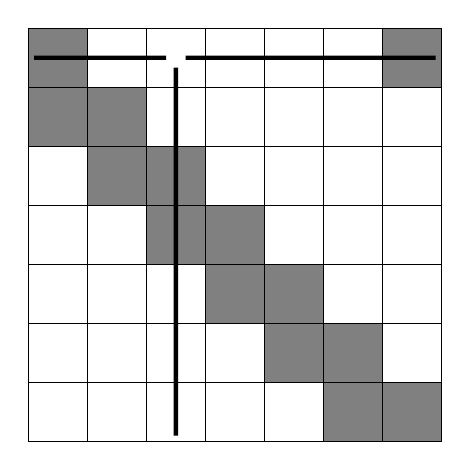
\begin{tikzpicture}[scale = 0.75]
    \foreach \i in {0,...,6} { \fill[gray] (\i, 6 - \i) rectangle (\i + 1, 7 - \i); }
    \foreach \i in {1,...,6} { \fill[gray] (\i-1, 6 - \i) rectangle (\i, 7 - \i); }
    \fill[gray] (6, 6) rectangle (7, 7);
    \draw (0,0) grid (7,7);
    \node (R) at (2.5, 6.5) {\huge\symrook};
    \draw[ultra thick]
      (0.1,6.5) -- (R) -- (6.9,6.5)
      (R) -- (2.5,0.1)
    ;
  \end{tikzpicture}
  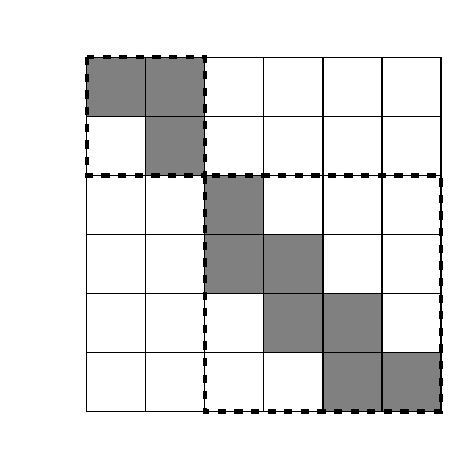
\begin{tikzpicture}[scale = 0.75]
    \path (0,-0.5) -- (0,6.5); % vertically center.
    \foreach \i/\j in {1/5, 2/5, 2/4, 3/3, 3/2, 4/2, 4/1, 5/1, 5/0, 6/0} { \fill[gray] (\i, \j) rectangle (\i + 1, \j + 1); }
    \draw[ultra thick, dashed] (1,6) rectangle (3,4) rectangle (7,0);
    \draw (1,0) grid (7,6);
  \end{tikzpicture}
  \caption[The derived board for a prefix of a m\'enage permutation of length $1$.]{
    The first chessboard shows a placement of a rook at position $3$,
    the second shows the remaining squares, and the third shows a permutation
    of the rows to put the board into a block-diagonal form.
  }
  \label{fig:menageSinglePlacement}
\end{figure}


Now we will give a name to these blocks,
which are illustrated in Figure \ref{fig:blockShape}.

\begin{definition}
  A board is called \textbf{staircase-shaped} if it matches one of the
  following four shapes:
  \begin{alignat*}{2}
    \mathcal{O}_{2n-1}           &= \{(i,i) : i \in [n]\}    &&\cup\ \{(i,i+1) : i \in [n-1]\} \\
    \mathcal{O}_{2n-1}^\intercal &= \{(i,i) : i \in [n]\}    &&\cup\ \{(i+1,i) : i \in [n-1]\} \\
    \mathcal{E}_{2n-2}           &= \{(i,i) : i \in [n-1]\}\ &&\cup\ \{(i+1,i) : i \in [n-1]\} \\
    \mathcal{E}_{2n-2}^\intercal &= \{(i,i) : i \in [n-1]\}\ &&\cup\ \{(i,i+1) : i \in [n-1]\},
  \end{alignat*}
  the subscripts represent the number of cells, and the names represent their
  parity.
  \label{def:staircaseShaped}
\end{definition}

\begin{lemma}
  For $\ell \geq 1$, and prefix $\alpha = (\alpha_1, \alpha_2, \dots, \alpha_\ell)$
  the derived complementary board $B_\alpha^c$ can be partitioned into
  disjoint staircase-shaped boards.
  \label{lemma:boardShape}
\end{lemma}
\begin{proof}
  The proof proceeds by induction on the length of the prefix.

  To establish the base case, consider a prefix of length $\ell = 1$.
  Because of the m\'enage restriction,
  $\alpha_1 \in \{2, 3, \dots, n-1\}$, and
  the derived complimentary board $B_{(\alpha_1)}^c$
  can be partitioned into two disjoint blocks with shapes
  $A_{\alpha_1 - 1}$ and $A^\intercal_{n - \alpha_1}$.
  (This is illustrated for the case of $n = 7$ and $\alpha_1$ in Figure \ref{fig:menageSinglePlacement}.)

  The inductive hypothesis is that the derived complimentary board for
  a prefix of length $\ell - 1$ consists of blocks with shape
  $A_{n_1}$, $A^\intercal_{n_2}$, $B_{n_3}$, or $B^\intercal_{n_4}$.
  Placing a rook in row $\ell$ can remove a top row or a column or both in a
  given block.
  Table \ref{table:rooksInBlocks} below
  shows the resulting blocks after placing a rook in
  $\ell$-th row of $B$,
  which may be in the top row or the $i$-th column of a given block.

  \begin{tabular}{|l|l|l|l|l|}
  \hline
  Rook placement
    & $\mathcal{O}_{2n-1}$
    & $\mathcal{O}_{2n-1}^\intercal$
    & $\mathcal{E}_{2n-2}$
    & $\mathcal{E}_{2n-2}$
  \\ \hline
  Row $1$
    & $\mathcal{O}_{2n-3}$
    & $\mathcal{E}_{2n-2}^\intercal$
    & $\mathcal{O}_{2n-3}$
    & $\mathcal{E}_{2n-4}^\intercal$
  \\
  Column $i$
    & $\mathcal{O}_{2i-3}$, $\mathcal{E}_{2n-2i}$
    & $\mathcal{E}_{2i-2}$, $\mathcal{O}_{2n-2i-1}^\intercal$
    & $\mathcal{E}_{2i-2}$, $\mathcal{E}_{2n-2i-2}$
    & $\mathcal{O}_{2i-3}$, $\mathcal{O}_{2n-2i-1}^\intercal$
  \\
  Row $1$, column $i$
    & $\mathcal{O}_{2i-5}$, $\mathcal{E}_{2n-2i}$
    & $\mathcal{O}_{2i-3}$, $\mathcal{O}_{2n-2i-1}^\intercal$
    & $\mathcal{O}_{2i-3}$, $\mathcal{E}_{2n-2i-2}$
    & $\mathcal{O}_{2i-5}$, $\mathcal{O}_{2n-2i-1}^\intercal$
  \\ \hline
  \end{tabular}
  \captionof{table}{
    The results of placing a rook in the first row, $i$-th column, or both
    for all staircase-shaped boards.
  }
  \label{table:rooksInBlocks}
  Therefore placing any number of rooks in the first $\ell$ results in a board
  of one of the four described shapes.
\end{proof}

\begin{figure}[ht!]
  \center
  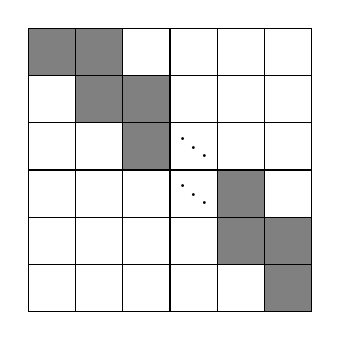
\begin{tikzpicture}[scale=0.6]
    \foreach \i/\j in {1/5, 2/5, 2/4, 3/4, 3/3, 5/2, 5/1, 6/1, 6/0} { \fill[gray] (\i, \j) rectangle (\i + 1, \j + 1); }
    \node at (4.5,3.65) {$\ddots$};
    \node at (4.5,2.65) {$\ddots$};
    \draw (1,0) grid (7,6);
  \end{tikzpicture}
  ~
  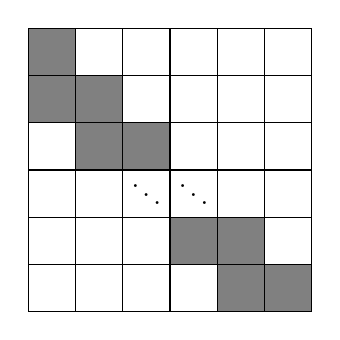
\begin{tikzpicture}[scale=0.6]
    \foreach \i/\j in {1/5, 1/4, 2/4, 2/3, 3/3, 4/1, 5/1, 5/0, 6/0} { \fill[gray] (\i, \j) rectangle (\i + 1, \j + 1); }
    \node at (3.5,2.65) {$\ddots$};
    \node at (4.5,2.65) {$\ddots$};
    \draw (1,0) grid (7,6);
  \end{tikzpicture}
  ~
  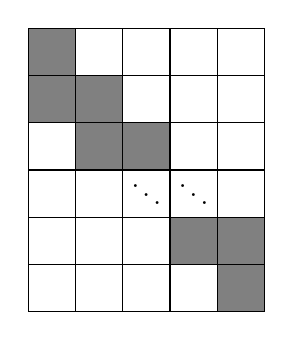
\begin{tikzpicture}[scale=0.6]
    \foreach \i/\j in {1/4, 1/5, 2/3, 2/4, 3/3, 4/1, 5/0, 5/1} { \fill[gray] (\i, \j) rectangle (\i + 1, \j + 1); }
    \node at (3.5,2.65) {$\ddots$};
    \node at (4.5,2.65) {$\ddots$};
    \draw (1,0) grid (6,6);
  \end{tikzpicture}
  ~
  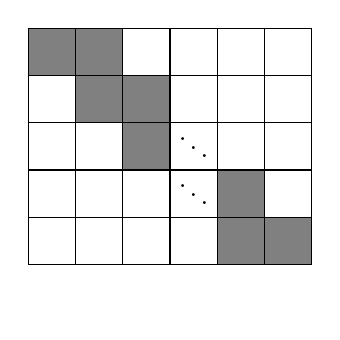
\begin{tikzpicture}[scale=0.6]
    \foreach \i/\j in {1/5, 2/5, 2/4, 3/4, 3/3, 5/2, 5/1, 6/1} { \fill[gray] (\i, \j) rectangle (\i + 1, \j + 1); }
    \node at (4.5,3.65) {$\ddots$};
    \node at (4.5,2.65) {$\ddots$};
    \path (1,0) grid (7,6);
    \draw (1,1) grid (7,6);
  \end{tikzpicture}
  \caption[Block shapes for a m\'enage permutation.]{
    Four boards, two $n \times n$ board with $2n - 1$ grey cells,
    a $n \times n-1$ board with $2n - 2$ grey cells, and a
    $n-1 \times n$ board with $2n - 2$ grey cells.
    We call them $A_n$, $A^\top_n$, $B_n$, and $B^\top_n$ respectively.
  }
  \label{fig:blockShape}
\end{figure}


\subsection{Rook polynomials of blocks}
Recall that the goal of partitioning $B$ into disjoint boards $b_1, b_2, \dots, b_m$
is so that we can factor $p_B(x)$ in terms of $p_{b_i}(x)$. Of course, this is
only helpful if we can describe $p_{b_i}(x)$, which is the goal of this section.
Thankfully, the rook polynomial of each $b_i$ will turn out to depend only on the
number of squares, $|b_i|$, which can be computed easily because of its structure.

We will begin by defining a family of polynomials that, suggestively, will turn
out to be the rook polynomials that we are looking for. This family is nearly
described by OEIS sequence A011973 \cite{oeis}.
\begin{definition}
  For $j \geq 0$, the $j$th \textbf{Fibonacci polynomial} $F_{j}(x)$ is defined recursively as:
  \begin{align}
    F_0(x) &= 1 \\
    F_1(x) &= 1 + x \\
    F_n(x) &= F_{n-1}(x) + xF_{n-2}(x).
  \end{align}
\end{definition}

\begin{lemma}
  If $B$ is a staircase-shaped board with $k$ squares, then
  $B$ has rook polynomial $p_{B}(x) = F_{k}(x)$ which agrees with the $k$-th
  Fibonacci polynomial.
\end{lemma}
\begin{proof}
  We will recall the recursive construction of rook polynomials from
  Lemma \ref{lemma:rookPolynomialRecursion}, and proceed by
  induction on the number of squares, always choosing to include or exclude
  the upper-left square.

  Since the reflections of board has the same rook polynomial as the
  unreflected board, without loss of generality, we
  will compute the rook polynomials for
  $\mathcal{O}_{2n-1}$ and $\mathcal{E}_{2n-2}$ respectively.

  % $A_n$ as our choice for the odd case and
  % $B_n$ as our choice for the even case.

  To establish a base case, consider the rook polynomials when $n = 1$, so
  the even board has $|\mathcal{E}_{0}| = 0$ squares and
  the odd board has $|\mathcal{O}_{1}| = 1$ square.
  We can see the corresponding rook polynomials directly. There is $1$ way to
  place $0$ rooks on $\mathcal{E}_{0}$ and no ways to place more rooks;
  similarly there is
  $1$ way to place $0$ rooks on $\mathcal{O}_{1}$,
  $1$ way to place $1$ rooks on $\mathcal{O}_{1}$, and
  no ways to place more than one rook. Thus \begin{alignat}{2}
    p_{\mathcal{E}_{0}}(x) &= 1     &&= F_0(x), \text{ and} \\
    p_{\mathcal{O}_{1}}(x) &= 1 + x &&= F_1(x).
  \end{alignat}

  With the base case established, our inductive hypothesis is that
  $p_{B}(x) = F_{h}(x)$ for
  whenever $B$ is a
  staircase-shaped boards with $h < k$ squares.



  % Even case
  Assume that we have $k$ squares where $k$ is even, so our board looks like
  $\mathcal{E}_{k}$. We can either place a rook or not in the upper-left square.
  If we include the square, then $(\mathcal{E}_{k})_i \cong \mathcal{E}_{k-2}$,
  if we exclude the square, then $(\mathcal{E}_{k})_e \cong \mathcal{O}_{k-1}$.
  Thus by Lemma \ref{lemma:rookPolynomialRecursion}, the rook polynomial of
  $\mathcal{E}_{k}$ is
  \begin{align}
    p_{\mathcal{E}_{k}}(x)
    &= xp_{\mathcal{E}_{k-2}}(x) + p_{\mathcal{O}_{k-1}}(x) \\
    &= xF_{k-2}(x) + F_{k-1}(x) \\
    &= F_{k}(x).
  \end{align}

  % Odd case
  The case where $k$ is odd proceeds in almost the same way.
  Here our board looks like $\mathcal{O}_{k}$.
  We can either place a rook or not in the upper-left square.
  If we include the square, then $(\mathcal{O}_{k})_i \cong \mathcal{O}_{k-2}$,
  if we exclude the square, then $(\mathcal{O}_{k})_e \cong \mathcal{E}_{k-1}$.
  Again by Lemma \ref{lemma:rookPolynomialRecursion}, the rook polynomial
  of $\mathcal{O}_{k}$ is
  \begin{align}
    p_{\mathcal{O}_{k}}(x)
    &= xp_{\mathcal{O}_{k-2}}(x) + p_{\mathcal{E}_{k-1}}(x) \\
    &= xF_{k-2}(x) + F_{k-1}(x) \\
    &= F_{k}(x).
  \end{align}
\end{proof}

\subsection{Prefix to block sizes}
Here's the idea: we group the uncrossed columns.

\begin{lemma}
  Given a prefix $\alpha = (\alpha_1, \alpha_2, \dots, \alpha_\ell)$
  and $i \not\in \alpha$,
  the number of cells of $B^c$ in column $i$ that do not have
  a first coordinate in $[\ell]$
  is given by the rule:
  \begin{equation}
    c_i = \begin{cases}
      0 & i < \ell \\
      1 & i = k \text{ or } i = n \\
      2 & \ell < i < n
    \end{cases}
  \end{equation}
\end{lemma}

\begin{proof}
  TODO: This almost follows from the description?
\end{proof}

Now we can put these column counts together based on the continuous blocks.

\begin{lemma}
  TODO:
  Partition $[n] \setminus \alpha$ into contiguous parts.
  This naturally partitions $B^c_\alpha$ into disjoint boards.
  The size of these boards is $\sum_{x \in \textrm{part}} c_x$.
  (this is what I've been calling our ``composition'')
\end{lemma}

\begin{figure}[ht!]
  \center
  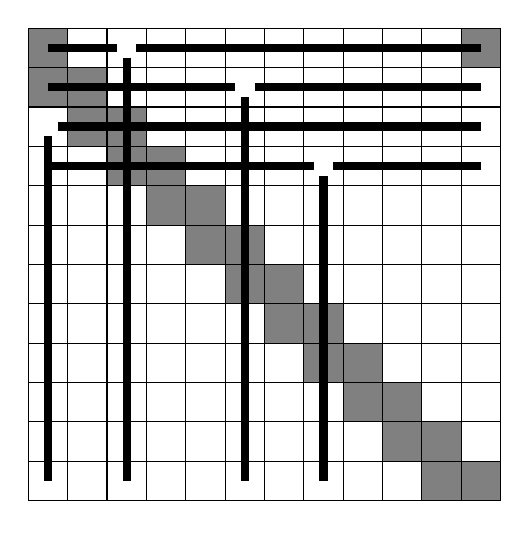
\begin{tikzpicture}[scale = 0.5]
    \path (0,-0.5) -- (0,6.5);
    \foreach \i in {0,...,11} { \fill[gray] (\i, 12-\i) rectangle (\i + 1, 11 - \i); }
    \foreach \i in {0,...,10} { \fill[gray] (\i, 11-\i) rectangle (\i + 1, 10 - \i); }
    \fill[gray] (11,11) rectangle (12,12);
    \draw (0,0) grid (12,12);
    \node (R1) at (2.5, 11.5) {\Large\symrook};
    \node (R2) at (5.5, 10.5) {\Large\symrook};
    \node (R3) at (0.5, 9.5) {\Large\symrook};
    \node (R4) at (7.5, 8.5) {\Large\symrook};
    \draw[line width = 3]
      (0.5,11.5) -- (R1) -- (11.5,11.5)
      (R1) -- (2.5,0.5)
    ;
    \draw[line width = 3]
      (0.5,10.5) -- (R2) -- (11.5,10.5)
      (R2) -- (5.5,0.5)
    ;
    \draw[line width = 3]
      (R3) -- (11.5,9.5)
      (R3) -- (0.5,0.5)
    ;
    \draw[line width = 3]
      (0.5,8.5) -- (R4) -- (11.5,8.5)
      (R4) -- (7.5,0.5)
    ;
  \end{tikzpicture}
  ~~~
  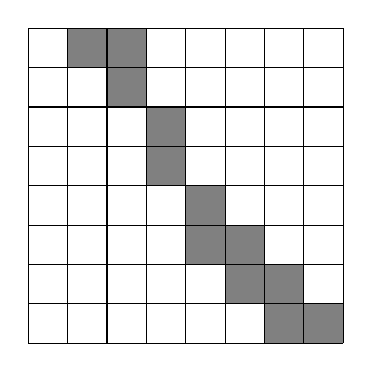
\begin{tikzpicture}[scale = 0.5]
    \path (0,-0.5) -- (0,6.5);
    \foreach \i/\j in {1/7, 2/6, 2/7, 3/4, 3/5, 4/2, 4/3, 5/2, 5/1, 6/1, 6/0, 7/0} {
      \fill[gray] (\i, \j) rectangle (\i + 1, \j + 1);
    }
    \draw (0,0) grid (8,8);
  \end{tikzpicture}
  ~~~
  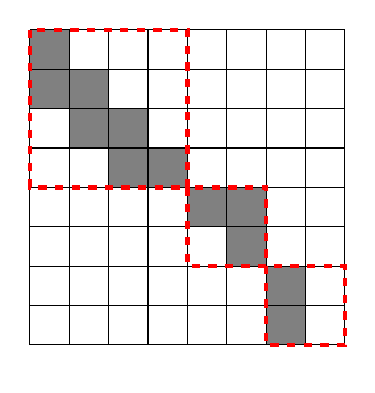
\begin{tikzpicture}[scale = 0.5]
    \path (0,-0.5) -- (0,6.5);
    \foreach \i/\j in {0/7, 0/6, 1/6, 1/5, 2/5, 2/4, 3/4, 4/3, 5/3, 5/2, 6/1, 6/0} {
      \fill[gray] (\i, \j) rectangle (\i + 1, \j + 1);
    }
    \draw (0,0) grid (8,8);
    \draw[ultra thick, dashed, red]
      (0,8) rectangle (4,4)
      (4,4) rectangle (6,2)
      (6,2) rectangle (8,0)
    ;
  \end{tikzpicture}
  \caption{
    xxx
  }
  \label{fig:partitionFromPrefix}
\end{figure}


\subsection{Complementary polynomials to m\'enage permutations with a given prefix}
Recap: We've taken a prefix, used it to find contiguous regions, used these to
find disjoint sub-boards related to $B_\alpha^c$, whose rook polynomials we know.
Now it's time to take these to count our number of m\'enage permutations with
the aforementioned prefix.
\begin{lemma}
  Given a board $B_\alpha^c$ that is partitioned into disjoint boards
  $b_1, b_2, \dots, b_m$, the rook polynomial of $B_\alpha^c$ is \[
    p_{B_\alpha^c}(x) = \prod_{i = 1}^m F_{b_i}(x).
  \]
\end{lemma}
\begin{proof}
  This follows directly from Lemma (TODO: rook polynomials of blocks)
  and Lemma (TODO: product of blocks is whole thing).
\end{proof}

Now that we know $p_{B_\alpha^c}$, we can use Lemma
(TODO: Complementary to original) to determine how many
m\'enage permutations there are with a given prefix. Because of Lemma
(TODO: all we need is the prefix to unrank), we have an algorithm to unrank.

\begin{example}
  Illustrating this particular example is too big to be of much interest, so
  here's a smaller example. There are $A000179(8) = 4738$ m\'enage
  permutations on $8$ letters. We'll use this algorithm to find the one
  at index $1000$.
  \begin{table}
    \center
    \begin{tabular}{|l|r|l|c|l|}
      \hline
      $\alpha$ & $\#\operatorname{prefix}(\alpha)$ & index range & composition & $\operatorname{unrank}_{i}(\alpha, \ell)$\\ \hline
      $1       $ & $0$   & $(0,0]$            & $-$       & $\operatorname{unrank}_{1000}(1,0)$          \\
      $2       $ & $787$ & $(0,787]$          & $(1,11)$  & $\operatorname{unrank}_{1000}(2,0)$          \\
      $3       $ & $791$ & $(787, 1578]$      & $(3,9)$   & $\operatorname{unrank}_{1000}(3,787)$        \\ \hline
      $31      $ & $0$   & $(787, 787]$       & $-$       & $\operatorname{unrank}_{1000}(31,787)$       \\
      $32      $ & $0$   & $(787, 787]$       & $-$       & $\operatorname{unrank}_{1000}(32,787)$       \\
      $33      $ & $0$   & $(787, 787]$       & $-$       & $\operatorname{unrank}_{1000}(33,787)$       \\
      $34      $ & $159$ & $(787, 946]$       & $(1,7)$   & $\operatorname{unrank}_{1000}(34,787)$       \\
      $35      $ & $166$ & $(946, 1112]$      & $(1,2,5)$ & $\operatorname{unrank}_{1000}(35,946)$       \\ \hline
      $351     $ & $24$  & $(946, 970]$       & $(0,2,5)$ & $\operatorname{unrank}_{1000}(351,946)$      \\
      $\cdots$   & $0$   & $(970,970]$        & $-$       & \\
      $354     $ & $34$  & $(970, 1004]$      & $(0,5)$   & $\operatorname{unrank}_{1000}(354,970)$      \\ \hline
      $3541    $ & $5$   & $(970,975]$        & $(0,5)$   & $\operatorname{unrank}_{1000}(3541,970)$     \\
      $3542    $ & $5$   & $(975,980]$        & $(0,5)$   & $\operatorname{unrank}_{1000}(3542,975)$     \\
      $\cdots$   & $0$   & $(980,980]$        & $-$       & \\
      $3546    $ & $8$   & $(980,988]$        & $(0,3)$   & $\operatorname{unrank}_{1000}(3546,980)$     \\
      $3547    $ & $10$  & $(988,998]$        & $(0,2,1)$ & $\operatorname{unrank}_{1000}(3547,988)$     \\
      $3548    $ & $6$   & $(998,1004]$       & $(0,4)$   & $\operatorname{unrank}_{1000}(3548,998)$     \\ \hline
      $35481   $ & $1$   & $(998,999]$        & $(0,4)$   & $\operatorname{unrank}_{1000}(35481,998)$    \\
      $35482   $ & $1$   & $(999,1000]$       & $(0,4)$   & $\operatorname{unrank}_{1000}(35482,999)$    \\ \hline
      $354821  $ & $0$   & $(999,999]$        & $(3)$     & $\operatorname{unrank}_{1000}(354821,999)$   \\
      $\cdots$   & $0$   & $(999,999]$        & $-$       & \\
      $354827  $ & $1$   & $(999,1000]$       & $(0,1)$   & $\operatorname{unrank}_{1000}(354827,999)$   \\ \hline
      $3548271 $ & $1$   & $(999,1000]$       & $(0)$     & $\operatorname{unrank}_{1000}(3548271,999)$  \\ \hline
      $35482716$ & $1$   & $(999,1000]$       & $()$      & $\operatorname{unrank}_{1000}(35482716,999)$ \\ \hline
    \end{tabular}
    \caption[Steps for computing the $1000$th m\'enage permutation in $S_8$.]{
      The recursive computation of the 1000th m\'enage permutation.
    }
  \end{table}
\end{example}

\section{Generalizations and Open Questions}
\subsection{Other restricted permutations}
Doron Zeilberger considers a more general family of restricted permutations.
\begin{definition}[\cite{Zeilberger2014}]
  Let $S \subset \mathbb Z$, then a \textit{$S$-avoiding permutation} is a
  permutation $\pi \in S_n$ such that \[
    \pi(i) - i - s \not\equiv 0 \bmod n \text{ for all } i \in [n] \text{ and } s \in S.
  \]
\end{definition}

\begin{example}
  Ordinary permutations are $\emptyset$-avoiding permutations,
  derangements are $\{0\}$-avoiding permutations, and
  we've defined menag\'e permutations as $\{-1,0\}$-avoiding permutations.

  The results in this paper generalize pretty easily to $\{i,i+1\}$-avoiding
  permutations for all $i$.
\end{example}

\subsection{Observation about Lyndon Words after? a given prefix}
\begin{definition}
  A \textit{Lyndon word} is a string that is the unique minimum with respect
  to all of its rotations.
\end{definition}
\begin{example}
  $00101$ is a Lyndon word because
  $00101 = \min\{00101, 01010, 10100, 01001, 10010\}$ is the unique minimum of
  all of its rotations.

  $011011$ is not a Lyndon word because while $011011 = \min\{011011, 110110, 101101, 011011, 110110, 101101\}$,
  it is not the \textbf{unique} minimum.
\end{example}
\begin{conjecture}
  Let $\mathcal{E}^{-1}$ denote the inverse Euler transform.
  Then the number of length $n+1$ Lyndon words that start with a prefix
  $\alpha$ follows a ``simple'' linear recurrence for sufficiently large $n$.
\end{conjecture}


% Using single-space for reference list.
\begin{singlespace}
% Bibliography
\phantomsection
\addcontentsline{toc}{chapter}{References}%
\markboth{References}{References}%
% If you use BibLaTeX
\printbibliography[title=References]
% If you use BibTeX
% \bibliographystyle{plain}
% \bibliography{references}
\end{singlespace}

% Appendices
\setcounter{section}{0} % Work around for weird Appendix numbering.
\phantomsection
\addcontentsline{toc}{chapter}{Appendices}%
\markboth{Appendices}{Appendices}%
\chapter*{Appendices}
\renewcommand\thesection{\Alph{section}}
\renewcommand*{\thesubsection}{\Alph{section}.\arabic{subsection}}
\begingroup
\numberwithin{equation}{section}
% Appendix source files
\section{A Long Proof}
\label{app:long_proof}

\subsection{Haskell Algorithm for M\'enage}
\begin{verbatim}
  import Helpers.Factorials (factorial)
  import Data.List (sort, nub)

  type Prefix = [Int]
  type PolynomialCoeffs = [Integer]
  type PrefixCount = Prefix -> Integer

  rookCount :: Int -> Integer -> Prefix
  rookCount n = unrank n n (rookPrefixCount n)

  -- unrank from alphabet of size n with k letters
  -- and a way of counting the number of words with a given prefix
  unrank :: Int ->                 -- Alphabet of n letters
            Int ->                 -- Words of length k
            (Prefix -> Integer) -> -- #prefix function
            Integer ->             -- Unrank at i
            Prefix                 -- Word at rank i
  unrank n k prefixCounter i = recurse (0, 0) 1 [] where
    recurse :: (Integer, Integer) -> -- index range for prefix (a, b]
               Int ->                -- candidate for current letter
               Prefix ->             -- established prefix
               Prefix                -- word at index
    recurse (a, b) c prefix
      | c > n              = error "Out of range!"
      | length prefix == k = prefix
      | a < i && i <= b    = recurse (a, b') 1 (prefix  ++ [c])
      | otherwise          = recurse (b, b'') (c + 1) prefix where
      b'      = a + prefixCounter (prefix ++ [c, 1])
      b''     = b + prefixCounter (prefix  ++ [c + 1])

  -- Assumes prefix is valid; no duplicate values or illegal positions.
  -- If n = 9 and the prefix is [3, 8, 7]
  -- This should return [[1,2],[4,5,6],[9]]
  getColGroups :: Int -> Prefix -> [[Int]]
  getColGroups n prefix = filter (not . null) $ colGroups where
    cols = 0 : (sort prefix) ++ [n+1]
    colGroups = zipWith (\a b ->  [a+1..b-1]) cols (tail cols)

  blockSizesFromPrefix :: Int -> Prefix -> [Int]
  blockSizesFromPrefix n prefix = map (sum . map colCells) colGroups where
    colGroups = getColGroups n prefix
    k = length prefix
    colCells c
      | c < k      = 0
      | c == k     = 1
      | c == n     = 1
      | otherwise  = 2

  fibonacciPoly :: Int -> PolynomialCoeffs
  fibonacciPoly = (!!) fibonacciPolynomials where
    fibonacciPolynomials = [1] : [1] : recurse [1] [1] where
      recurse f g = h : recurse g h where
        h = ([0,1] .*. f) .+. g

  complementaryRookPolynomial :: Int -> Prefix -> PolynomialCoeffs
  complementaryRookPolynomial n prefix = foldr (.*.) [1] blockPolys where
    blockPolys = map (\i -> fibonacciPoly (i + 1)) blockSizes where
      blockSizes = blockSizesFromPrefix n prefix

  invalidPrefix :: Int -> Prefix -> Bool
  invalidPrefix n prefix = containsDuplicates || invalidPosition where
    containsDuplicates = prefix /= (nub prefix)
    invalidPosition = any inRestrictedPosition $ zip [0..] prefix where
      inRestrictedPosition (i, x) = (x `mod` n == i) || (x == i + 1)

  rookPrefixCount :: Int -> Prefix -> Integer
  rookPrefixCount n prefix
    | invalidPrefix n prefix = 0
    | otherwise      = recurse 0 crp where
    n' = fromIntegral (n - length prefix)
    crp = complementaryRookPolynomial n prefix
    recurse k (c:cs) = (-1)^k * c * factorial (n'-k) + recurse (k+1) cs
    recurse _ [] = 0

  -- The polynomial a + bx + cx^2 ... is represented as
  -- [a, b, c, ...]
  -- These are helper functions for adding and multiplying polynomials
  (.+.) :: PolynomialCoeffs -> PolynomialCoeffs -> PolynomialCoeffs
  (.+.) p1 [] = p1
  (.+.) [] p2 = p2
  (.+.) (a:p1) (b:p2) = (a + b) : (p1 .+. p2)

  (.*.) :: PolynomialCoeffs -> PolynomialCoeffs -> PolynomialCoeffs
  (.*.) p1 [] = []
  (.*.) [] p2 = []
  (.*.) p1 p2 = foldr1 (.+.) termwiseProduct where
    termwiseProduct = map f $ zip [0..] p1 where
      f (i, x) = replicate i 0 ++ map (*x) p2
\end{verbatim}


\Blindtext[1]

\endgroup


% In case your dissertation has multiple volumes.
% \addvolumecontents{thesis_part2}
% \addvolumecontents{thesis_part3}
% \addvolumecontents[lof]{thesis_part2}

\end{document}
